% =============================================================================
%   Bachelor's Thesis — Bio-Inspired Foveation in DeepGaze III
%   Imer Itez · Goethe-Universität Frankfurt am Main · 2026
%
%   Build:
%       latexmk -pdf -interaction=nonstopmode main.tex
%
%   Source repository: https://github.com/W00DSRULES/bio-inspired-foveation-in-dg3
% =============================================================================
\documentclass[
  paper=a4,
  fontsize=11pt,
  twoside=false,
  % The thesis is printed single-sided and bound on the left edge, where the
  % binding swallows part of the margin. BCOR is taken off the paper width
  % before the type area is computed and added back to the left margin, so the
  % text block sits 10mm further right: 37mm of margin on the left against 27mm
  % on the right. DIV goes from 10 to 11 at the same time, which hands the type
  % area back the width BCOR took off it — without that the line gets 5% shorter
  % and the reflow pushes a further eight paragraphs past the right edge.
  BCOR=10mm,
  DIV=11,
  parskip=half,
  numbers=noenddot,
  bibliography=totoc,
  listof=totoc,
  open=any,
  chapterprefix=true,
]{scrreprt}

% --- Encoding and language -----------------------------------------------
\usepackage[utf8]{inputenc}
\usepackage[T1]{fontenc}
\usepackage{lmodern}   % scalable Type1 font (required for microtype expansion)
\usepackage[british]{babel}
\usepackage{csquotes}
\usepackage{microtype}
% The binding correction takes 8mm off the line, which pushed a handful of
% paragraphs holding unbreakable file paths past the right edge. This lets
% TeX loosen a paragraph rather than let a line stick out.
\setlength{\emergencystretch}{2em}

% --- Math ---------------------------------------------------------------
\usepackage{amsmath, amssymb, amsthm}
\usepackage{mathtools}

% --- Graphics and tables ------------------------------------------------
\usepackage{xcolor}
\usepackage{xspace}
\usepackage{graphicx}
\usepackage{float}      % [H] to pin a figure inside the section that owns it
% Every figure comes from the repo's results/ directory — there is no
% thesis-only artwork, by design: a figure the repo cannot regenerate is a
% figure the thesis cannot defend. Paths resolve from the location of main.tex.
% notebooks/README.md maps each committed figure to what reproduces it.
% ../results/ holds figures generated by this project's own code; figures-external/
% holds figures reproduced from published papers (see its README for sources).
\graphicspath{{../results/}{figures-external/}}
\usepackage{booktabs}
\usepackage{caption}
\usepackage{subcaption}

% Float placement. The defaults are tuned for sparse figures; Chapters 2-4 are
% figure-dense enough that figures queued up and surfaced several pages after
% the text that refers to them. Allowing a fuller float page and more floats per
% text page keeps each figure near its discussion.
\setcounter{topnumber}{3}
\setcounter{bottomnumber}{2}
\setcounter{totalnumber}{4}
\renewcommand{\topfraction}{0.85}
\renewcommand{\bottomfraction}{0.6}
\renewcommand{\textfraction}{0.1}
\renewcommand{\floatpagefraction}{0.7}
% A page holding only floats gets its floats pushed to the top rather than
% centred between two blocks of white space.
\makeatletter
\setlength{\@fptop}{0pt}
\makeatother
\usepackage{tikz}
\usetikzlibrary{positioning, arrows.meta, fit, backgrounds}

% --- File paths ---------------------------------------------------------
% \texttt{} sets a path as one unbreakable word: TeX breaks lines at spaces and
% hyphens, and hyphenates nothing inside typewriter text, so a path with no
% space in it either fits on the line or runs off the page. \pth{} is url.sty's
% breaking machinery with a typewriter face, which lets a line break after
% "/", "_" and "." — the separators a path already has. Underscores are literal
% inside it, so paths are written as they appear on disk, without \_ escapes.
\usepackage{url}
\DeclareUrlCommand\pth{\urlstyle{tt}}
% url.sty's defaults break after "/", "_", "." and "="; a module:function
% reference needs the colon and a flag needs the hyphen as well.
\makeatletter
\g@addto@macro\UrlBreaks{\do\:\do\-}
\makeatother

% --- Hyperlinks ---------------------------------------------------------
\usepackage[
  colorlinks=true,
  linkcolor=black,
  citecolor=blue!50!black,
  urlcolor=blue!50!black,
  pdftitle={Bio-Inspired Foveation in DeepGaze III},
  pdfauthor={Imer Itez},
]{hyperref}

% --- Bibliography (biber + biblatex, author-year) -----------------------
\usepackage[
  backend=biber,
  style=authoryear,
  natbib=true,
  maxcitenames=2,
  uniquelist=false,
  date=year,
  isbn=false,
  url=false,
]{biblatex}
\addbibresource{bibliography.bib}

% \citeyearpar prints a bare year, which the model table of ch02 uses so that each
% row's name carries its own reference. biblatex leaves that year unlinked, so it
% is redeclared here to wrap it in the same hyperlink every other citation gets.
% extradate is dropped with it: two Kummerer 2015 entries make biblatex print
% "2015a", and in a table row whose sibling "2015b" never appears the suffix reads
% as a typo. The model name disambiguates the row, and the link still resolves.
\DeclareCiteCommand{\citeyearpar}[\mkbibparens]
  {}
  {\bibhyperref{\printfield{year}}}
  {\multicitedelim}
  {}

% --- Custom macros ------------------------------------------------------
% =============================================================================
%   macros.tex — thesis-wide commands and notation
% =============================================================================

% --- Project shorthands -------------------------------------------------
\newcommand{\dg}{DG3\xspace}                                % DeepGaze III

% --- Foveation notation ------------------------------------------------
\newcommand{\fov}[1]{\ensuremath{#1_{\text{fov}}}}          % subscript-fov on anything
\newcommand{\ppd}{\mathrm{ppd}}                            % pixels per degree (viewing geometry)

% --- Vector / norm notation --------------------------------------------
\newcommand{\vect}[1]{\mathbf{#1}}
\newcommand{\norm}[1]{\left\|#1\right\|}
\newcommand{\fixxy}{(\mathrm{fix}_x, \mathrm{fix}_y)}       % current fixation point

% --- Probability & information theory ----------------------------------
\newcommand{\E}{\mathbb{E}}                                 % expectation
\newcommand{\R}{\mathbb{R}}
\newcommand{\IG}{\mathrm{IG}}                               % Information Gain
\newcommand{\LL}{\mathrm{LL}}                               % Log-Likelihood
\newcommand{\NSS}{\mathrm{NSS}}
\newcommand{\AUC}{\mathrm{AUC}}                             % Area Under the Curve

% --- Cross-reference shortcuts (saves typing "Figure~\ref{...}") -------
\newcommand{\figref}[1]{Figure~\ref{fig:#1}}
\newcommand{\tabref}[1]{Table~\ref{tab:#1}}
\newcommand{\eqnref}[1]{Equation~(\ref{eq:#1})}
\newcommand{\chref}[1]{Chapter~\ref{ch:#1}}
\newcommand{\secref}[1]{Section~\ref{sec:#1}}
\newcommand{\subsecref}[1]{Section~\ref{subsec:#1}}

% --- Editorial markers (visible TODO / WIP / draft notes) --------------
%   Usage: \todo{rewrite this paragraph}. Switched off for the final PDF;
%   to see markers again while drafting, use the two commented definitions.
\newcommand{\todo}[1]{}
\newcommand{\note}[1]{}
% \newcommand{\todo}[1]{\textcolor{red}{\textbf{[TODO: #1]}}}
% \newcommand{\note}[1]{\textcolor{blue}{\emph{[note: #1]}}}


% --- Metadata -----------------------------------------------------------
\title{Bio-Inspired Foveation in DeepGaze III}
\author{Imer Itez}

% =============================================================================
\begin{document}

\begin{titlepage}
  \centering
  \vspace*{2cm}
  {\Large Goethe-Universit\"at Frankfurt am Main \par}
  \vspace{0.5cm}
  {\large Department of Computer Science\par}
  \vspace{2.5cm}
  {\Huge\bfseries Bio-Inspired Foveation in \par}
  \vspace{0.3cm}
  {\Huge\bfseries DeepGaze III \par}
  \vspace{2cm}
  {\Large Bachelor's Thesis \par}
  \vspace{1.5cm}
  {\large submitted by \par}
  \vspace{0.3cm}
  {\Large Imer Itez \par}
  \vfill
  {\large Supervisor: \emph{Prof.\ Dr.\ Matthias Kaschube}\par}
  \vspace{0.2cm}
  {\large Advisor: \emph{Santiago Galella}\par}
  \vspace{0.3cm}
  {\large 18 August 2026 \par}
\end{titlepage}

\cleardoublepage
% ----- Front matter (abstract, acknowledgements, ToC) -------------------
\chapter*{Abstract}
\addcontentsline{toc}{chapter}{Abstract}
DeepGaze III is a model of human gaze that predicts, from the image and the fixations already made,
where the next fixation will land, reading the whole image at uniform resolution. A human sees
sharply only a small region around the point of gaze and chooses every saccade from a degraded
peripheral preview. This thesis asks whether DeepGaze III depends on peripheral detail the humans it
predicts never had. A gaze-contingent foveation after Geisler and Perry re-blurs the model's input
around its current fixation before every prediction. Copies of the model are fine-tuned on MIT1003 and
compared on held-out images: one on sharp input, one on foveated input, and one with the same blur
pinned to the image centre, the last two repeated at cutoffs below human acuity. At human acuity the
sharp and foveated models differ by under 1\% of what the sharp model gains over the centerbias, so
the foveation costs nothing this experiment can measure. Blurring below
human acuity does cost, mainly in how sharply the model concentrates its probability rather than in
how it ranks locations. At the coarsest cutoff the fixed-centre model sits $0.013$~bits below the
gaze-contingent one, so letting the sharp region follow the gaze returns part of what degrading the
periphery takes away. Across the 1003 images the model's fit varies more than any two models differ,
and follows how far the fifteen subjects spread. The finding rests on one dataset of fifteen adults
and one fixed acuity falloff, and may not transfer beyond them; the front-end built here is what a
wider test would use.
\cleardoublepage
\chapter*{Acknowledgements}
\addcontentsline{toc}{chapter}{Acknowledgements}
I would like to thank Santiago Galella and Prof.\ Dr.\ Matthias Kaschube for their supervision and for the opportunity they gave me to work on this thesis.

Anneme ve babama, verdikleri manevi destek ve motivasyon için teşekkür ederim.

\bigskip
\begin{quote}
\itshape
We shall not cease from exploration\\
And the end of all our exploring\\
Will be to arrive where we started\\
And know the place for the first time.
\end{quote}
\begin{flushright}
--- T.\,S.\ Eliot, \emph{Four Quartets} (\enquote{Little Gidding})
\end{flushright}

\bigskip
\begin{quote}
\itshape
The true method of knowledge is experiment.
\end{quote}
\begin{flushright}
--- William Blake, \emph{All Religions are One}
\end{flushright}

\cleardoublepage
\tableofcontents

% `listof=totoc` in the class options puts both lists into the table of
% contents; no \addcontentsline is needed.
\cleardoublepage
\listoffigures

\cleardoublepage
\listoftables

\cleardoublepage
\chapter*{List of Vocabulary}
\addcontentsline{toc}{chapter}{List of Vocabulary}

The terms this thesis uses in a fixed sense, with the meaning each one carries throughout.

\begin{description}

\item[Arm] One condition of the experiment, run on one kind of input. The arms are identical in
  everything else, so a difference between them comes from the input.

\item[AUC] Area under the curve. The probability that the model ranks a fixated pixel above a pixel drawn
  at random from the same image. It measures ranking alone, so any rescaling of the map leaves it
  unchanged.

\item[Backbone] The frozen DenseNet-201 that turns an image into features. Pretrained for object
  recognition and never updated here.

\item[Centerbias] The fixed prior map of where fixations fall irrespective of image content.
  Free-viewing gaze concentrates near the centre of the stimulus, and information gain is measured
  against this prior.

\item[Consensus region] The part of an image that at least a given fraction of the subjects fixated
  within $2^\circ$ of. The figures draw it as a contour to show where the population agreed; it is
  not one of the reported measures.

\item[Cortical magnification] The disproportionate share of visual cortex given to the central visual
  field.

\item[Crowding] The failure to identify an object in peripheral vision when other objects lie close to
  it, even where the object on its own would be resolvable.

\item[\dg{}] DeepGaze III, the model this thesis modifies. Given an image and the recent fixations it
  returns a probability map for the next fixation.

\item[Dose--response] Ordering the arms by foveation strength to see whether a cost grows with it,
  rather than testing one strength on its own.

\item[Eccentricity] Angular distance from the point of gaze, in degrees of visual angle. Acuity falls as
  it grows.

\item[Epoch] One pass of training over every training image.

\item[Fixation] A period during which gaze rests at one location. Every metric here is computed per
  fixation.

\item[Fixation entropy $H_{\text{fix}}$] How spread out the subjects' fixations were on one
  image: the entropy of their pooled fixation counts over a $16 \times 16$ grid, normalised to
  $[0, 1]$. It describes the people, not the model, and is the per-image dispersion measure this
  work reports. Distinct from map entropy, which describes one prediction.

\item[Fold] One of ten partitions of the dataset into training, validation and test images. Every
  scanpath of an image lands in the same fold, so a test image is never seen during training.

\item[Fovea] The small central region of the retina with the highest receptor density, covering about
  two degrees.

\item[Foveal cutoff $f_{c0}$] The highest spatial frequency resolvable at the centre of gaze, in cycles
  per degree. It sets the strength of the foveation, and the human value is about $40$.

\item[Foveation] Reducing image resolution with distance from the point of gaze, in imitation of the
  eye.

\item[Free viewing] Looking at an image with no specific target or task given.

\item[Gaze-contingency term] The difference between the gaze-contingent and the fixed-centre arm at the
  same foveal cutoff. Both carry the identical blur, so the term is what following the gaze contributes
  with the amount of blur held constant.

\item[Gaze-contingent] Re-centred on the current fixation before every forward pass, so the sharp region
  follows the gaze.

\item[Information gain (IG)] Log-likelihood measured against the centerbias rather
  than against a uniform map, in bits per fixation. Zero means the model adds nothing beyond the tendency
  to look near the centre. $\Delta \IG$ is the difference in information gain between two arms scored on
  the same fixations.

\item[Inhibition of return] The reduced likelihood of gaze returning to a location fixated recently.

\item[Log-likelihood (LL)] The probability the model assigned to the fixations the subjects made, in
  bits per fixation against a uniform map.

\item[Map entropy] The entropy $-\sum p \log_2 p$ of a predicted probability map, summed over its pixels
  and reported in bits. It measures how widely the model spreads its density, irrespective of where the
  peak sits.

\item[MIT1003] An eye-tracking dataset of 1003 natural images, each freely viewed for three seconds
  by up to fifteen subjects while eye position was recorded.

\item[Mode distance] The distance in pixels from the peak of the predicted probability map to the true
  fixation.

\item[NSS] Normalised scanpath saliency. The predicted value at fixated pixels once the map has been
  rescaled to zero mean and unit standard deviation.

\item[Nyquist frequency] The highest spatial frequency a sampled image can carry, half its sampling
  rate. Blur that removes only frequencies above it leaves the stored image unchanged.

\item[Paired difference] A comparison taken between two arms on the same fold and the same fixations, so
  that variation in image difficulty cancels.

\item[Pearson's $r$] The correlation between two per-image quantities read from their values, measuring
  how closely the pairs sit on a straight line.

\item[Pixels per degree ($\ppd$)] How many image pixels span one degree of visual angle at the viewing
  geometry. It converts the acuity model from degrees to pixels, and is $35$ for MIT1003.

\item[Priority map] A map of where attention should be directed, combining stimulus-driven salience with
  task and history.

\item[Probability map] \dg{}'s output, the probability at each pixel that the next fixation lands there.

\item[Read-out] The three small trainable networks above the frozen backbone (the released model carries ten copies of them, averaged). They are the only part
  fine-tuned here.

\item[Saccade] The rapid eye movement between two fixations. Vision is suppressed while it happens.

\item[Saliency map] A map of how conspicuous each image location is on stimulus properties alone.

\item[Scanpath] One subject's fixations on one image, in the order they were made.

\item[Sharp] Not foveated. The input the control arm receives.

\item[Sharp radius] The eccentricity out to which the foveated frame stays identical to the original,
  because the eye out-resolves the display there.

\item[Space-variant] Applying a different amount of blur at each pixel rather than one amount to the
  whole frame.

\item[Spatial priority network] \dg{}'s own name for the read-out component that turns backbone features
  into a stimulus-driven map.

\item[Spearman's $\rho$] Pearson's correlation computed on ranks, each value replaced by its position
  among the 1003 stimuli, so it asks only whether the two orderings agree.

\item[Subject] One of the fifteen people whose gaze MIT1003 recorded.

\item[Validation split] The fold used to choose the learning rate, check that training behaved, and
  compute the diagnostics. It is distinct from the test fold, which carries the main comparison.

\end{description}


\cleardoublepage
% ----- Main matter ------------------------------------------------------
\chapter{Introduction}
\label{ch:introduction}

Where people look in a scene is not random. Human subjects converge on faces, text and salient objects
\citep{judd2009mit1003}. \emph{Where} attention lands is one question; in \emph{what order} it
lands is another. Computational models of gaze predict these from the image, fitted to eye-tracking
recordings of people looking at photographs. The earlier ones predicted only where, marking the regions
of an image that draw fixations. DeepGaze~III \citep{kummerer2022deepgaze3}, \dg{} hereafter, addresses
the second, the free-viewing \emph{scanpath} (\figref{intro-scanpath}). It predicts a probability density
over the next fixation given the image and the recent history, and is evaluated at the level of that
distribution rather than by matching individual sampled paths \citep{kummerer2021state}.

\begin{figure}[tbp]
  \centering
  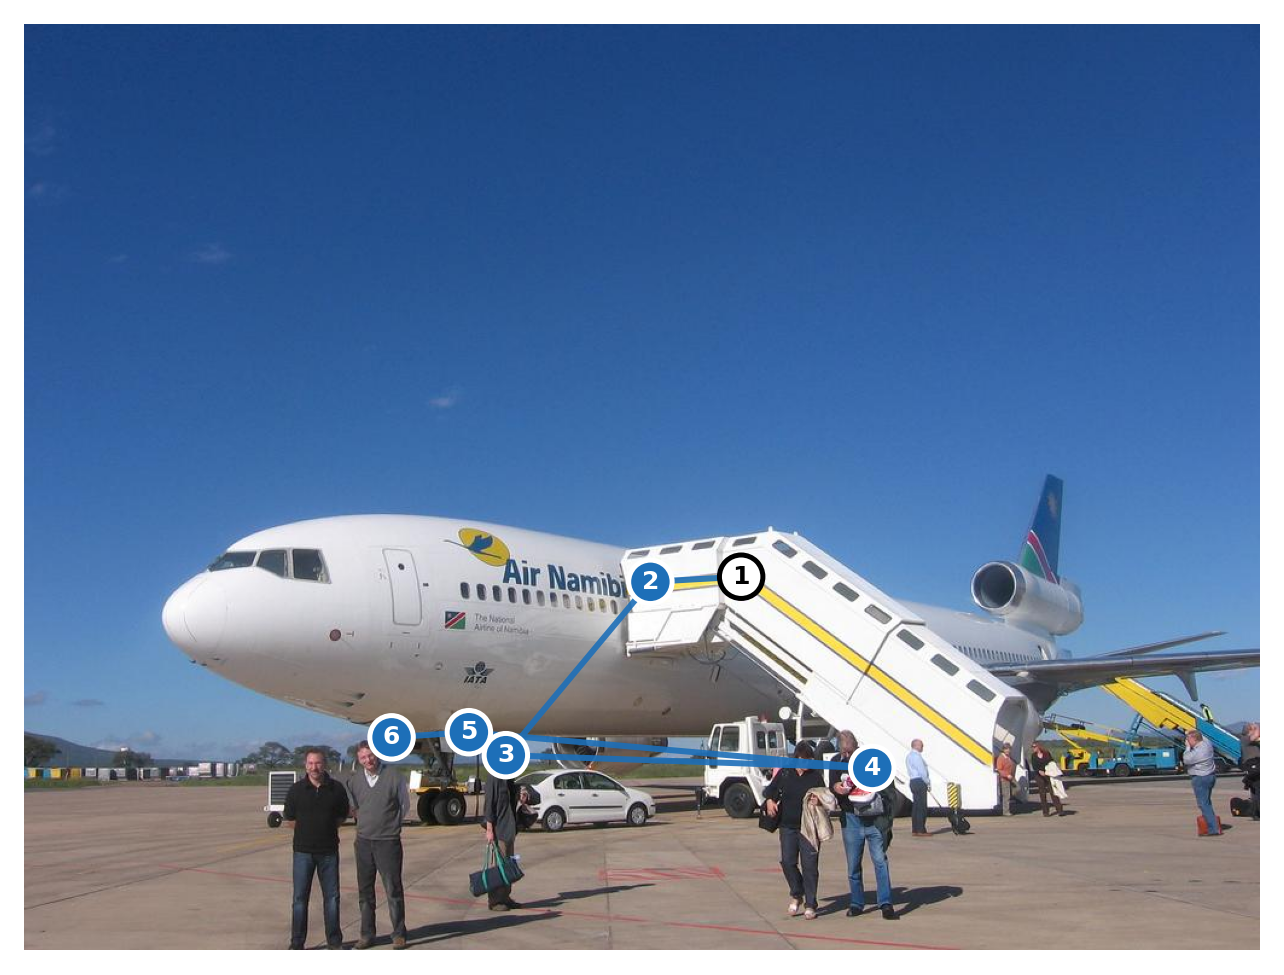
\includegraphics[width=0.72\textwidth]{foveation_mit1003/intro_scanpath_stim0091.png}
  \caption[A human scanpath on an MIT1003 image]{One subject's fixations on an MIT1003 image \citep{judd2009mit1003}, numbered in viewing
    order (the first in white): the boarding stairs, the airline name, then the people on the tarmac.}
  \label{fig:intro-scanpath}
\end{figure}

Human vision is foveated, with acuity high only in a
small region around the point of gaze, falling steeply with eccentricity. That is why the eyes move, bringing
each region of interest onto the high-acuity fovea, with the choice of where to look next made from a
low-resolution peripheral preview \citep{najemnik2005}. \dg{} instead reads the whole image at uniform
resolution, so its predictions can be driven by fine detail a foveated viewer could not perceive.
Whether \dg{} needs that detail is the question this thesis puts to it.

This thesis narrows that gap at the input. A gaze-contingent, space-variant foveation after
\citet{geislerperry1998} re-blurs the model's input around its current fixation before every forward pass
--- sharp at gaze, blurred in the periphery --- so the model must predict each saccade
from the degraded peripheral preview a human would have had. Two otherwise-identical models, one trained on sharp
input and one on foveated input, are compared on MIT1003 \citep{judd2009mit1003} under image-stratified
cross-validation, alongside a third arm that pins the same blur to the image centre and so
separates gaze-contingency from the loss of peripheral resolution. At human acuity foveating the input costs
nothing the experiment can measure. A cost appears once the falloff is pushed past human
acuity, and grows as it steepens. Holding the same blur at the image centre costs more than letting it
follow the gaze, and the gap grows as the periphery is degraded further.
Alongside the foveation experiment, a per-image diagnostic shows
that \dg{}'s fit varies more from image to image than any arm differs from another. Future work sets out a
developmental question, whether a model's learning trajectory recapitulates the development of human
gaze across age.

\section{Applications}
\label{sec:intro-applications}

The mechanism and the measurement bear on problems outside the one asked here. \citet{geislerperry1998}
built the falloff this thesis borrows in order to send video over a low-bandwidth link, keeping detail
only where the eye was pointed. Gaze-tracked displays now do the same inside the renderer, drawing the
periphery of a rendered frame at reduced cost \citep{guenter2012foveated, patney2016foveated} and
steering what is left of the budget with a predicted saliency map \citep{gao2025foveatedpathtracing}. A
scanpath model gives the next fixation as well as the current one, so the region about to be looked at
can be drawn sharply before the eye reaches it. \chref{results} measures how the fit to human fixations
changes as peripheral detail is discarded, which is that budget question in another form.

The same problem arises with no human eye in the loop. A robot or a vehicle can carry a wide
low-resolution camera for the field of view and a narrow high-resolution one that is steered, which
\citet{wloka2018starfc} identify as the engineering counterpart of the retina's own arrangement.
Something has to decide where the narrow camera points, and a model that predicts the next fixation is a
candidate for that decision. \citet{zhang2020gazereview} survey the use of recorded human gaze in
training agents that face this choice.

Predicting where people look is already used in design. \citet{judd2009mit1003} name advertising among
the applications of fixation prediction, and \citet{wloka2018starfc} note that commercial tools predict
the first several fixations, the short window of attention an advertisement receives. A scanpath model
states the order in which the parts of a layout are reached, so a designer can ask whether the brand is
fixated early and not only whether it stands out. Interface layouts have been studied the same way
\citep{jiang2024eyeformer}.

\section{Structure of this thesis}

\chref{background} reviews foveated vision and the lineage of saliency and scanpath models leading to
\dg{}. \chref{methods} describes the host architecture and where the foveation attaches, then defines the
evaluation framework, the multi-subject and per-image diagnostics, and the gaze-contingent foveation
mechanism with its training protocol. \chref{results} reports the foveation experiment across the sharp
control, the gaze-contingent arms and the fixed-centre arms, then the per-image
analysis. \chref{discussion} interprets the finding and the per-image diagnostic, states the
limitations (among them what the dataset does not record about its subjects) and sets out the work the
mechanism enables. \chref{conclusion} states what the experiment settles and what it leaves open.

\chapter{Background}
\label{ch:background}

% Background covers foveated vision, the saliency/scanpath lineage, foveated models and the
% \dg{} architecture. Dataset and metrics are defined where first used in \chref{methods};
% subject differences, including age, are in \chref{discussion}.

This thesis asks what happens to a model of where people look next when it is made to see the scene with
the resolution falloff of a human eye.

\section{Foveated vision}
\label{sec:foveated-vision}

Human vision is not uniform across the visual field. Acuity is highest at the \emph{fovea}, a region
roughly $2^\circ$ of visual angle in radius around the point of gaze, and falls off steeply with distance
from it into the periphery \citep{strasburger2011peripheral}. Only a small patch of any scene is seen
sharply at any instant.

This is why the eyes move. Looking at a scene is a cycle of \emph{fixations}, during which the eye is
nearly still and visual information is taken in, separated by \emph{saccades}, the fast jumps between
them, during which little is seen \citep{rayner1998eye}. Where to look next has to be chosen from what the
blurred periphery shows, together with memory of what was already inspected \citep{henderson2003gaze}.
\citet{najemnik2005} showed that human search is close to a Bayesian ideal observer that picks each
saccade to maximise the probability of finding the target, weighing every candidate fixation by what the
eccentricity-dependent visibility map would reveal from there.
\figref{one-fixation} shows one image sharp and at two foveation strengths.

\begin{figure}[tbp]
  \centering
  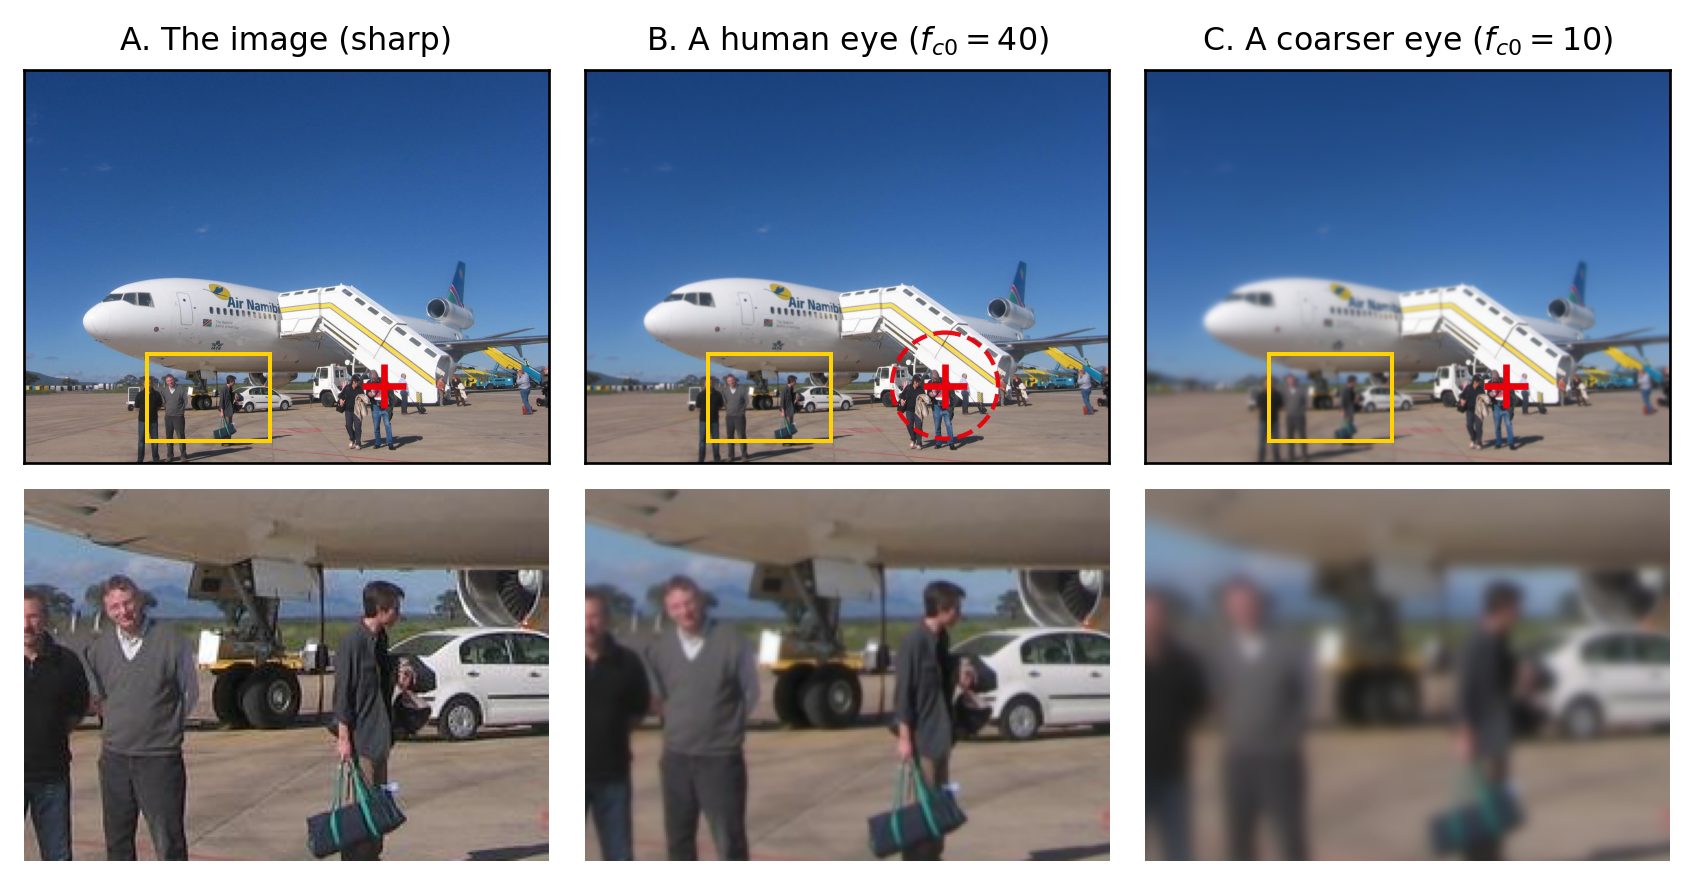
\includegraphics[width=\textwidth]{background/one_fixation.png}
  \caption[One image, sharp and foveated]{One image from MIT1003 \citep{judd2009mit1003}, sharp and foveated at two strengths, at the dataset's $35$ pixels per degree.
    The red cross is the fixation and the yellow box the patch magnified below. The dashed circle in
    B, of radius $3^\circ$, encloses the region the blur leaves untouched (\subsecref{sharp-radius});
    at $f_{c0} = 10$ no such region is left.}
  \label{fig:one-fixation}
\end{figure}

Detail is measured in cycles per degree, the number of repeats of a pattern that fit into one degree of
visual angle (a thumb held at arm's length covers about two degrees). The more repeats fit into that
degree, the finer the detail, and blurring an image removes the finest.

This thesis models the falloff as a cutoff spatial frequency that falls with eccentricity, following
\citet{geislerperry1998}, discarding at every point in the image the detail finer than the cutoff for
that eccentricity. The model folds into one curve the coarser retinal
sampling away from the fovea \citep{curcio1990photoreceptor} and the shrinking cortical area per degree
of visual field, called \emph{cortical magnification}
\citep{daniel1961representation, strasburger2011peripheral}. It
also treats the falloff as identical in every direction, whereas measured acuity differs between
directions in the visual field (\figref{retinal-falloff}). The shape of the falloff is set by one parameter, $e_2$, the eccentricity at which
the cutoff has halved. \chref{methods} uses $e_2 = 2.3^\circ$, the value \citet{geislerperry1998} fitted to human
contrast-sensitivity measurements.
The \citet{geislerperry1998} model is used here because one number sets its strength, the cutoff at the
point of gaze, $f_{c0}$, in cycles per degree. That number can be set to the human value, and below it to degrade
the periphery further than an eye does.
The blur models the loss of resolution only. Peripheral vision also loses in other ways, among them
crowding, the failure to identify an object when others lie close to it \citep{rosenholtz2016peripheral},
which the model leaves out (\secref{disc-limits}).

\begin{figure}[tbp]
  \centering
  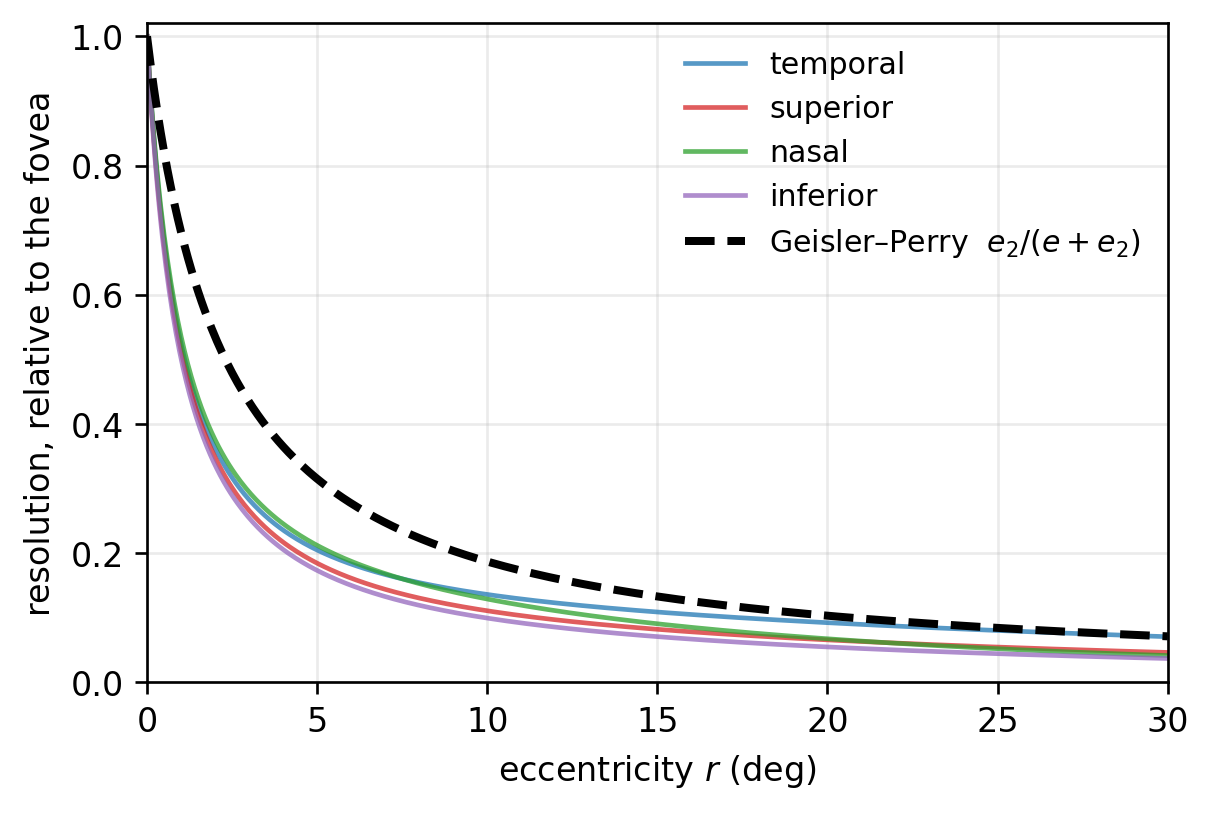
\includegraphics[width=0.72\textwidth]{background/retinal_falloff.png}
  \caption[The acuity model against measured falloff]{The model of \chref{methods} against the falloff it simplifies. The coloured curves are what
    \citet{watson2014formula}'s ganglion-cell density fit implies along the four directions out from
    the fovea; the dashed one is the Geisler--Perry cutoff used here, falling more slowly because it is
    fitted to what a subject can see rather than to what the retina samples.}
  \label{fig:retinal-falloff}
\end{figure}

\section{Saliency and scanpath models}
\label{sec:models}

A \emph{saliency map} is the spatial distribution of fixations; a \emph{scanpath} is their order. Both are
targets a gaze model can be asked to predict, and \figref{saliency-vs-scanpath} shows the same data under
each reading. \dg{} shows the two are not exclusive, computing a saliency map and using it to predict the next
fixation in a scanpath, but they still set different problems.

A saliency map can be built from the data itself, by collecting every fixation many subjects made on an
image and smoothing them together (\figref{saliency-vs-scanpath}A).

Scanpaths cannot be built that way. A saliency map has one value per pixel, and every recorded fixation
is evidence about one of them. A scanpath is an ordered sequence, so the same counting would need
evidence about each sequence a subject might produce; the number of possible sequences grows with their
length, while a dataset holds a handful per image. A scanpath model
therefore has to compute the next fixation from the image and the fixations so far, rather than look it
up.

\begin{figure}[tbp]
  \centering
  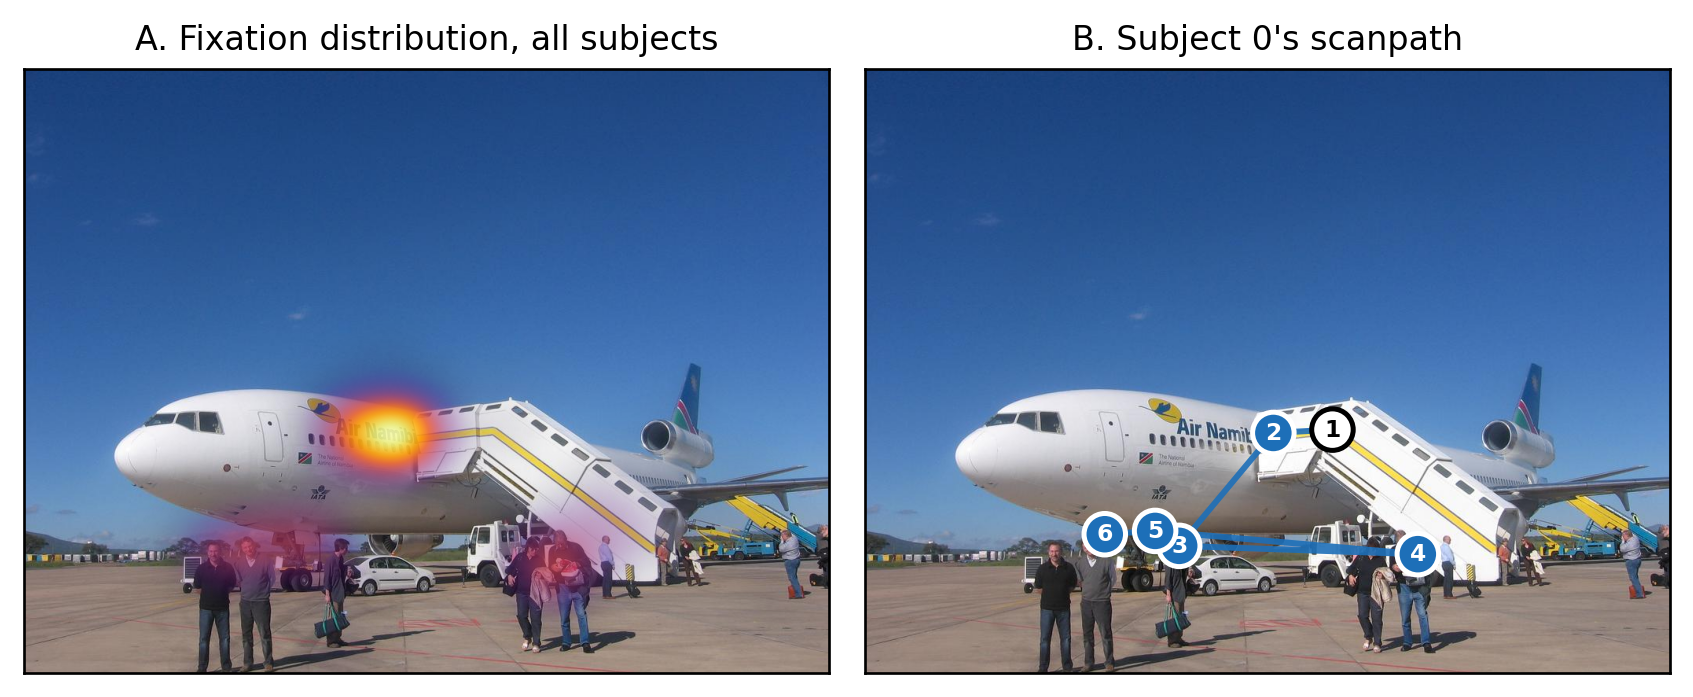
\includegraphics[width=\textwidth]{background/saliency_vs_scanpath.png}
  \caption[A saliency map and one scanpath]{One MIT1003 image \citep{judd2009mit1003} under the two readings. \textbf{A.} Every fixation of
    all fifteen subjects, smoothed into a density, with order discarded. \textbf{B.} One subject's
    fixations, numbered in viewing order.}
  \label{fig:saliency-vs-scanpath}
\end{figure}

The models below use \emph{saliency map} in a second, mechanistic sense, as bottom-up conspicuity computed
from the image alone, where a region stands out because it differs from its surroundings in contrast,
colour or orientation. The brain is thought to select saccade targets from a \emph{priority}
map, that same image-driven signal plus whatever the viewer's goals make relevant and a memory of
where they have already looked \citep{fecteau2006salience, zelinsky2015priority}.
\figref{dg3-composition} shows the two maps \dg{} adds to predict one fixation. Its probability map
has the image-driven signal and a memory of the fixations already made, and
\figref{history-conditioning} shows that memory changing the prediction as the history grows. The
goals have no counterpart in it, because the subjects of MIT1003 viewed each image freely with no
task set.

\begin{figure}[tbp]
  \centering
  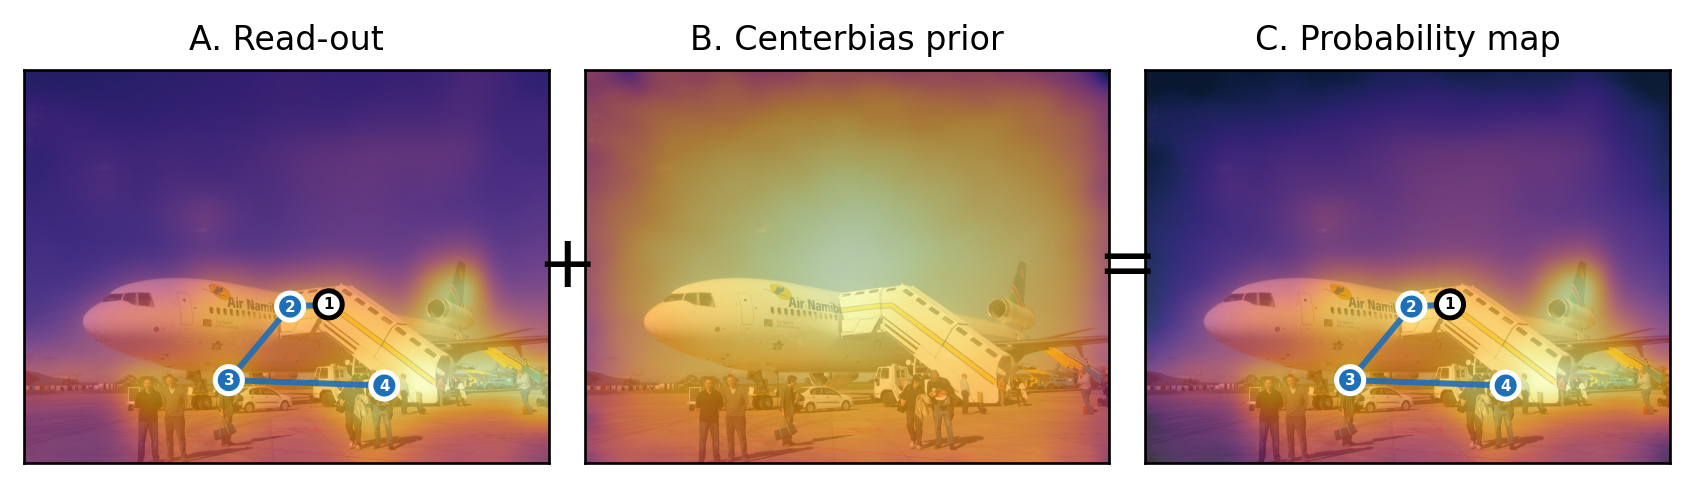
\includegraphics[width=\textwidth]{background/dg3_composition.png}
  \caption[\dg{} composing one prediction]{\dg{} given the first four fixations of one subject (drawn). \textbf{A.} The read-out's map,
    from the image and those fixations together. \textbf{B.} The centerbias (\secref{dg3-arch}),
    scaled by the weight the model learned. \textbf{C.} Their sum in log units, normalised. A and C
    share a colour scale; B carries its own.}
  \label{fig:dg3-composition}
\end{figure}

\dg{} reuses the convolutional read-out of the static DeepGaze line and adds conditioning on fixation
history, joining the two lines \figref{lineage} traces.

\begin{figure}[tbp]
  \centering
  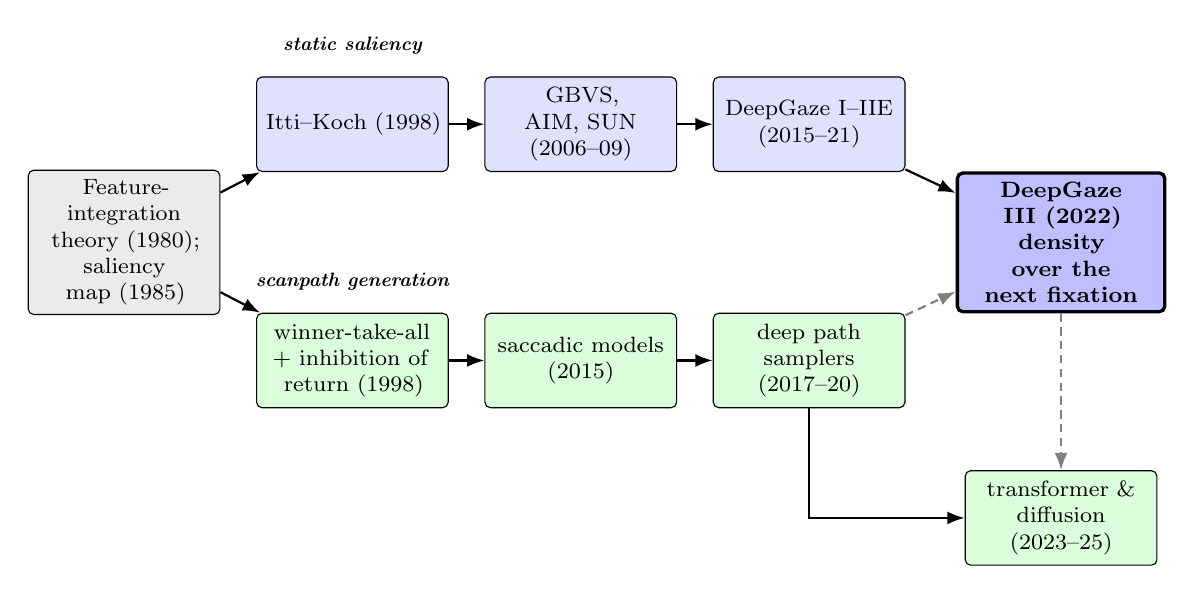
\begin{tikzpicture}[
    seed/.style  = {draw, rounded corners=2pt, fill=black!8, align=center,
                    font=\footnotesize, text width=22mm, minimum height=12mm},
    sal/.style   = {draw, rounded corners=2pt, fill=blue!12, align=center,
                    font=\footnotesize, text width=22mm, minimum height=12mm},
    scan/.style  = {draw, rounded corners=2pt, fill=green!14, align=center,
                    font=\footnotesize, text width=22mm, minimum height=12mm},
    host/.style  = {draw, very thick, rounded corners=2pt, fill=blue!25, align=center,
                    font=\footnotesize\bfseries, text width=24mm, minimum height=14mm},
    flow/.style  = {-{Latex[length=2.2mm]}, thick},
    graft/.style = {-{Latex[length=2.2mm]}, densely dashed, thick, gray},
    lane/.style  = {font=\scriptsize\bfseries\itshape, anchor=center},
  ]
    % --- lane labels ---
    \node[lane] at (2.9, 5.0)  {static saliency};
    \node[lane] at (2.9, 2.0)  {scanpath generation};

    % --- root ---
    \node[seed] (r1) at (0.0, 2.5) {Feature-integration\\ theory (1980);\\ saliency map (1985)};

    % --- static-saliency lineage ---
    \node[sal]  (s1) at (2.9, 4.0)  {Itti--Koch (1998)};
    \node[sal]  (s2) at (5.8, 4.0)  {GBVS, AIM, SUN\\ (2006--09)};
    \node[sal]  (s3) at (8.7, 4.0)  {DeepGaze I--IIE\\ (2015--21)};

    % --- scanpath-generation lineage ---
    \node[scan] (p1) at (2.9, 1.0)  {winner-take-all\\ + inhibition of\\ return (1998)};
    \node[scan] (p2) at (5.8, 1.0)  {saccadic models\\ (2015)};
    \node[scan] (p3) at (8.7, 1.0)  {deep path samplers\\ (2017--20)};

    % --- confluence and what follows ---
    \node[host] (dg) at (11.9, 2.5) {DeepGaze III (2022)\\ density over the\\ next fixation};
    \node[scan] (nx) at (11.9,-1.0) {transformer \&\\ diffusion (2023--25)};

    % --- succession within the two lineages ---
    \draw[flow] (r1) -- (s1);
    \draw[flow] (r1) -- (p1);
    \draw[flow] (s1) -- (s2);   \draw[flow] (s2) -- (s3);
    \draw[flow] (p1) -- (p2);   \draw[flow] (p2) -- (p3);

    % --- where the lineages meet ---
    \draw[flow]  (s3) -- (dg);
    \draw[flow]  (p3) |- (nx.west);
    \draw[graft] (p3) -- (dg);
    \draw[graft] (dg) -- (nx);
  \end{tikzpicture}
  \caption[Two lines of work, and where they meet]{Static saliency learns where people look on average; scanpath generation produces the order.
    \dg{} inherits the frozen-backbone read-out of the first and the history conditioning of the
    second. Solid arrows mark descent, dashed ones an idea carried across lines.}
  \label{fig:lineage}
\end{figure}

\subsection{From hand-crafted saliency to learned features}
\label{subsec:saliency-lineage}

\citet{treisman1980feature} set out the picture later models inherit. Simple
visual features are registered across the whole field at once, and attention is then
directed to one location at a time. Guided Search added that the second stage is steered
by the first rather than deployed blindly \citep{wolfe1989guided}.
\citet{koch1985shifts} turned Treisman's account into a mechanism whose parts are still in use: the
feature maps are combined into one topographic \emph{saliency map}, a winner-take-all
network selects its peak, and inhibiting that location briefly --- what was later named
\emph{inhibition of return} --- lets the next-most-active one win. They describe shifts of
attention rather than eye movements, but this is how later models read an ordered
sequence of fixations off a single map, as \citet{itti1998saliency} first implemented.

These are \emph{hand-crafted} models, in which a person chooses which features to compute and how
to weight them, and nothing is fitted to eye-tracking data. Because the
result emits both a map and a path, it is at once a saliency model and a saccade
generator. Later hand-crafted models kept the architecture and varied how activation
on the map was computed \citep{harel2006gbvs, bruce2009saliency, zhang2008sun}.

Deep Gaze~I \citep{kummerer2015deepgaze1} took the ImageNet feature maps of
\citet{krizhevsky2012alexnet}, left them untouched, and fitted only a small read-out on top
of them to human fixations. It reported the best results on the MIT Saliency Benchmark at the
time, without a face or text detector anywhere in the model, because the semantic content that draws
fixations was already in the features, which hand-crafted models had to supply through
purpose-built detectors. That fixed the recipe
the whole line then followed, and the one used here, freezing a pretrained network's
features and training only a small read-out on top of them
\citep{kummerer2016deepgaze2, linardos2021deepgaze2e}. Every model in this line,
hand-crafted or learned, emits a single static map, predicting \emph{where} fixations
land but not their order.

\subsection{Scanpath-prediction models}
\label{subsec:scanpath-lineage}

Scanpath models predict the fixation sequence itself. The earliest is the winner-take-all
with inhibition of return of \subsecref{saliency-lineage}, but it always jumps to the
current peak, so it produces one fixed path per image and reproduces neither the
variability of human gaze nor its \emph{oculomotor} regularities (how far and in which
direction people tend to move their eyes, independently of what the image contains). Those
regularities predict fixation locations at least as well as image salience does
\citep{tatler2009prominence}. Le~Meur and Liu built them in directly, drawing candidates from the saliency map
\emph{reweighted} by the measured human saccade amplitude and direction distributions and by a memory
term that suppresses locations just visited, rather than always taking the peak
\citep{lemeur2015saccadic}.

Deep models learn the dynamics instead, from saliency volumes sampled over time
\citep{assens2017saltinet} to \emph{inverse reinforcement learning} for goal-directed search
\citep{yang2020predicting}, which infers from human search paths what reward those paths were
maximising and then acts on it. These differ in machinery but all emit paths rather than a probability
for an observed fixation, so they are scored by how closely a sampled path resembles a human
one, through order-alignment metrics such as ScanMatch \citep{cristino2010scanmatch} and Sequence Score
\citep{yang2020predicting}.
\citet{kummerer2021state} show that path-to-path similarity can rank a \emph{wrong} model above the
true generating distribution. Human scanpaths on one image disagree with each other
(\figref{scanpath-variability}), so any single human path
is one draw from a broad distribution, and so is any single model path. Two draws from
the same distribution routinely look unalike, while a model that collapses onto one
stereotyped path can resemble each individual
human more closely than another human does. Scoring the density instead asks how much probability the
model placed where people looked, which variability cannot distort in that direction.

\begin{figure}[tbp]
  \centering
  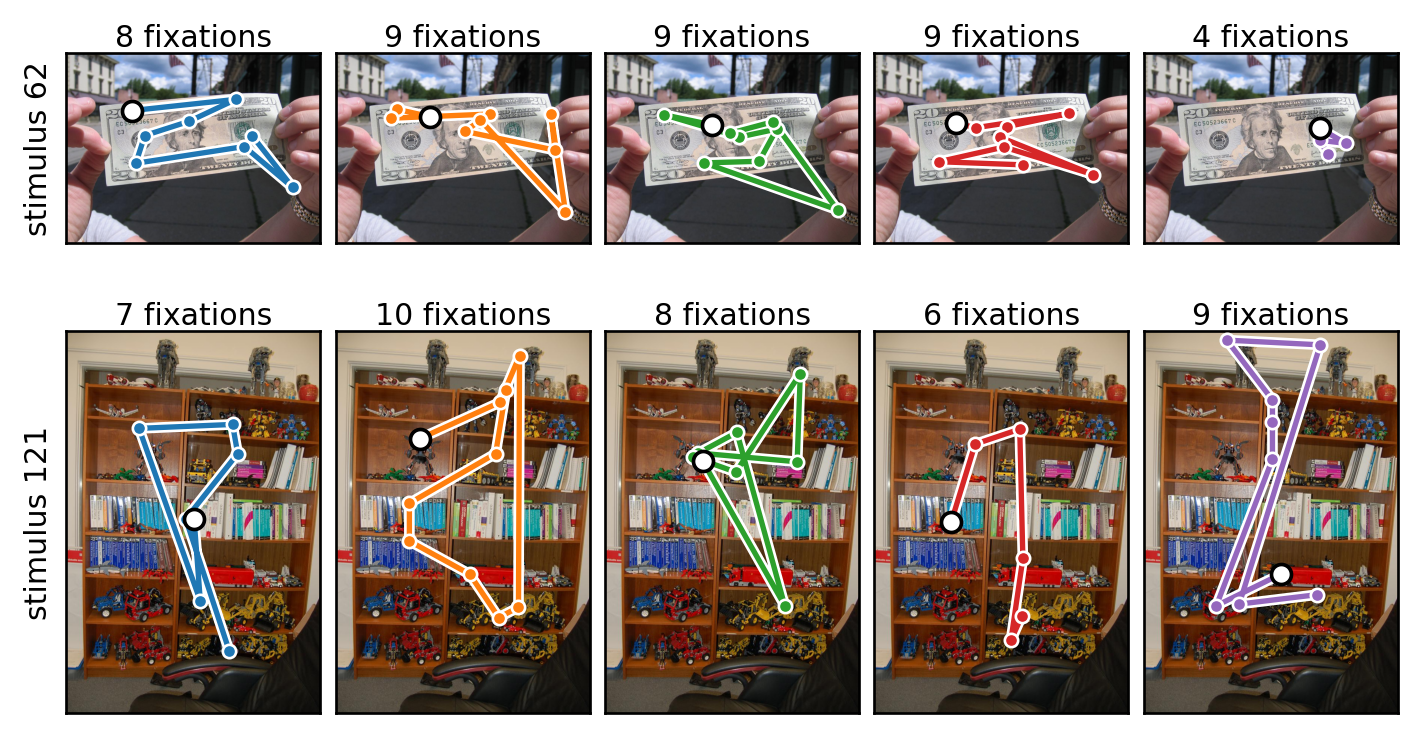
\includegraphics[width=\textwidth]{background/scanpath_variability.png}
  \caption[Scanpath variability between subjects]{The first five of the fifteen subjects on two stimuli, each panel one subject's fixations in
    viewing order with the first in white. \textbf{Top:} the same object, in different orders and
    with different fixation counts. \textbf{Bottom:} a dispersed stimulus, where the fixations land
    on different parts of the image from subject to subject.}
  \label{fig:scanpath-variability}
\end{figure}

\dg{} \citep{kummerer2022deepgaze3} closes that gap. Instead of producing a path, it produces a
probability for every location the next fixation could land on, given the image and the fixations so
far. That probability can be read at the place a person looked, so the model is scored on what it
predicted there rather than on how closely one of its paths resembles one of theirs. It is the model this thesis instruments, and \chref{methods} describes how it
is built. \figref{history-conditioning} shows what conditioning on the history does to the prediction.

\begin{figure}[tbp]
  \centering
  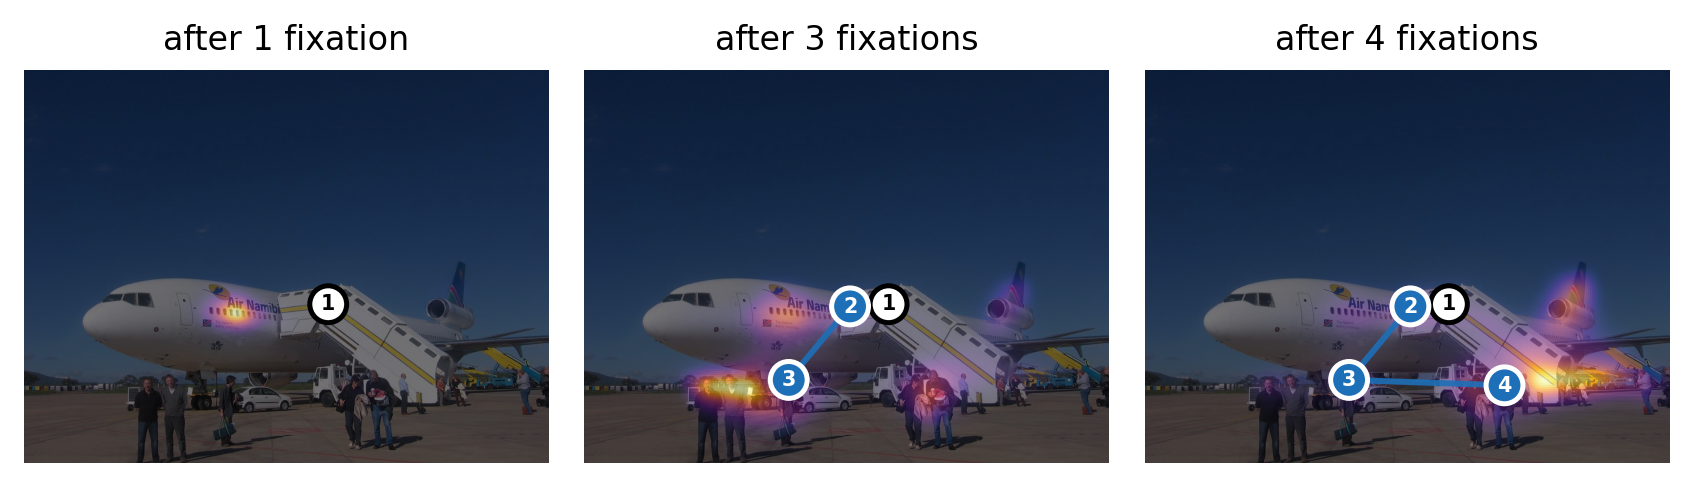
\includegraphics[width=\textwidth]{demos/priority_evolution/priority_evolution_stim0091.png}
  \caption[Conditioning on fixation history]{The probability map \dg{} predicts after $1$, $3$ and $4$ fixations of one subject's scanpath,
    with that scanpath overlaid. The path is the subject's, not a model sample, so each panel is where
    the model expected that subject to go next, and the gap between the two is what the likelihood of
    \subsecref{metrics} measures.}
  \label{fig:history-conditioning}
\end{figure}

\subsection{Current state (2023--2025)}
\label{subsec:contemporary}

Transformers \citep{vaswani2017attention, dosovitskiy2021vit} and diffusion models
\citep{ho2020ddpm} became standard tools across computer vision, and scanpath researchers
took them up as they arrived.

Gazeformer predicts
goal-directed search attention with a transformer that encodes the search target
through a language model, which lets it generalise to targets never seen in training
\citep{mondal2023gazeformer}. HAT unifies top-down search and bottom-up free-viewing
in a single transformer, predicting a dense heat-map per fixation where earlier models chose
from a coarse grid of cells; it is also the only model in this section with an explicit foveal
mechanism, which \secref{foveated-models} takes up \citep{yang2024hat}. EyeFormer uses a transformer policy trained by
reinforcement learning and adds personalisation, adapting to a handful of scanpaths from one subject
\citep{jiang2024eyeformer}. TPP-Gaze models fixation position and \emph{duration} jointly with neural
temporal point processes \citep{damelio2025tppgaze}, so a fixation's timing is a distribution. The
model here leaves timing out. ScanDiff uses a
diffusion model to generate \emph{diverse} scanpaths, taking the spread of plausible
paths as the thing to predict \citep{cartella2025scandiff}.

The transformer backbones carry a data cost. A transformer has none of the locality and translation
equivariance a convolution builds in, so it has to learn them, and \citet{dosovitskiy2021vit} report that
their model generalises worse than a comparable convolutional network when trained on ImageNet alone
and overtakes it only after pretraining on a dataset an order of magnitude larger. Several of the models
above are built for visual search rather than free viewing, a difference \secref{position} returns to.

\section{Foveated models}
\label{sec:foveated-models}

Most deep saliency and scanpath models read the whole image at uniform resolution. The few that
reintroduce a fovea differ in \emph{where} they attach it, and the subsections below take those places
in pipeline order.

\subsection{At the input}
\label{subsec:fov-input}

Input-space models degrade the image before the network sees it, by resampling or by blurring.

\emph{Resampling} takes closely
spaced samples near the fovea and progressively sparser ones outward, as the retina's own receptors are
spaced. Laying those samples back out on an even grid magnifies the centre and squeezes the periphery, so
straight lines bend and a pixel no longer sits where it came from. \citet{dacosta2024retinal} apply this
to a recognition network rather than a gaze model, but the transform is the same one a foveated gaze
model would inherit.

A space-variant \emph{blur} leaves every pixel exactly where it was and changes only
how sharp the picture is there, as SemBA-FAST does for semantic search \citep{luzio2025semba}. The search
model of \citet{yang2020predicting} uses a two-level version of the same idea, a sharp patch at the
fixation laid over a blurred copy of the whole frame. This thesis is input-space and uses the blur.

STAR-FC \citep{wloka2018starfc} is the closest prior work, the one input-space model that foveates for
free viewing, the task studied here. It re-applies a retinal transform at each new fixation and takes the
next fixation as the maximum of a priority map built from conspicuity and a history of visited locations.
It selects that maximum rather than emitting a density, so it emits ordered sequences and cannot be
scored by likelihood (\tabref{model-capabilities}). Its transform is the same space-variant blur, applied
anisotropically where the falloff here is identical in every direction. STAR-FC then splits the blurred
frame, running a low-level saliency algorithm over the periphery and a deep network over the centre; the
model here reads the whole foveated frame with one network.

\subsection{At the features}
\label{subsec:fov-features}

Feature-space models act on the network's internal representations. HAT reads
them at two resolutions, coarse over the whole frame and fine at each fixation, in what its authors call
a \enquote{simplified foveated retina} \citep{yang2024hat}. Because that stage sits \emph{after} the backbone,
the backbone still receives every detail, and the constraint governs only how the resulting features are
pooled.

\subsection{At the decision}
\label{subsec:fov-decision}

The SceneWalk lineage \citep{engbert2015scenewalk, schwetlick2019ccn, schwetlick2023diss} constrains the
selection step itself. SceneWalk drives its attention map by saliency
multiplied by a Gaussian window centred on the current gaze (\enquote{spatially-limited (foveated)
access}, so detail near fixation contributes more than the periphery), and subtracts a second map that
builds up at visited
locations to produce inhibition of return. Because the model emits a density, its parameters can be
fitted and its variants compared by likelihood \citep{schuett2017likelihood}, the same footing \dg{} is
evaluated on here.

The window weights the saliency signal inside a cognitive dynamical model, so the image is never
degraded and only the weight of each location in the decision changes.

\tabref{model-capabilities} puts the models of this chapter side by side.

\begin{table}[tbp]
  \centering
  \caption[What the models of this chapter predict, and where they foveate]{The models of this chapter,
    in order of publication, each name carrying the citation it is discussed under.
    \emph{Predicts} separates a
    single static map per image from an ordered sequence. \emph{Likelihood} marks the models that assign
    a probability to each observed fixation; the rest emit sampled paths and are compared by how
    closely a path resembles a human one (\subsecref{scanpath-lineage}). \emph{Foveation} names the
    stage at which a model imposes an eccentricity-dependent
    resolution limit, and \emph{follows gaze} marks the ones that re-centre that limit on the current
    fixation.}
  \label{tab:model-capabilities}
  \footnotesize
  \setlength{\tabcolsep}{2.5pt}
  \begin{tabular}{lccccc}
    \toprule
    model & task & predicts & likelihood & foveation & follows gaze \\
    \midrule
    Itti--Koch \citeyearpar{itti1998saliency}     & free viewing         & where + order & ---        & ---      & ---        \\
    Le~Meur \& Liu \citeyearpar{lemeur2015saccadic} & free viewing       & where + order & ---        & ---      & ---        \\
    SceneWalk \citeyearpar{engbert2015scenewalk, schwetlick2019ccn} & free viewing & where + order & \checkmark & decision & \checkmark \\
    DeepGaze I--IIE \citeyearpar{kummerer2015deepgaze1, linardos2021deepgaze2e} & free viewing & where & \checkmark & ---      & ---        \\
    SaltiNet \citeyearpar{assens2017saltinet}     & free viewing         & where + order & ---        & ---      & ---        \\
    STAR-FC \citeyearpar{wloka2018starfc}         & free viewing         & where + order & ---        & input    & \checkmark \\
    Yang et al.\ \citeyearpar{yang2020predicting} & search               & where + order & ---        & input    & \checkmark \\
    \dg{} \citeyearpar{kummerer2022deepgaze3}     & free viewing         & where + order & \checkmark & ---      & ---        \\
    Gazeformer \citeyearpar{mondal2023gazeformer} & search               & where + order & ---        & ---      & ---        \\
    HAT \citeyearpar{yang2024hat}                 & free viewing, search & where + order & \checkmark & features & \checkmark \\
    EyeFormer \citeyearpar{jiang2024eyeformer}    & free viewing         & where + order & ---        & ---      & ---        \\
    SemBA-FAST \citeyearpar{luzio2025semba}       & search               & where + order & \checkmark & input    & \checkmark \\
    TPP-Gaze \citeyearpar{damelio2025tppgaze}     & free viewing         & where + order & \checkmark & ---      & ---        \\
    ScanDiff \citeyearpar{cartella2025scandiff}   & free viewing, search & where + order & ---        & ---      & ---        \\
    \midrule
    this thesis                  & free viewing         & where + order & \checkmark & input    & \checkmark \\
    \bottomrule
  \end{tabular}
\end{table}

\section{Position of this thesis}
\label{sec:position}

\dg{}'s own authors raised the absence of foveation. Introducing the model,
\citet{kummerer2019ccn} write that \enquote{one might argue that our model is limited by the
fact that it is not foveated}. They answered it in the same paper and again in the journal version, at
the read-out, where several spatial priority channels do not perform substantially better than one
\citep{kummerer2019ccn, kummerer2022deepgaze3}. The input
was sharp in every variant, so what a foveated input does was left open, and it is the gap this thesis
occupies.

The successors of \subsecref{contemporary} change the generator (transformer,
diffusion, point process), and what they add over \dg{} is reach: a fixation history
without a fixed window, image regions that interact without depth, and in TPP-Gaze's case
fixation durations. The mechanism of \chref{methods} attaches ahead of the backbone, so it is
compatible with any of them.

Free viewing removes the goal input to target selection (\secref{models}), though not the subject's
contribution altogether, since faces, text and people are fixated more than image contrast predicts
\citep{judd2009mit1003}. Constraining what the stimulus delivers therefore bears directly on this task,
in a way it plausibly would not on search, where a model could still reason about where the target ought
to be.

The last row of \tabref{model-capabilities} pairs input foveation that follows gaze with free viewing
and a likelihood score, which no row above combines.

That fixes what the experiment asks of the model. \dg{} is trained and evaluated on input no human
subject could receive, with every pixel sharp, including the ones far enough from the modelled gaze that a
person would see only a blur. Restricting the input to what a foveated subject could resolve asks
whether that detail carries any of the model's fit to human fixations, and degrading the periphery
further asks how much the model draws on the coarse peripheral signal a viewer chooses saccades from
\citep{najemnik2005}; if it does, the cost should grow as the falloff steepens. \chref{methods} builds
the arms, and \chref{results} reports what the data show.

\chapter{Methods}
\label{ch:methods}

This chapter specifies the experiment. \secref{dg3-arch} describes the host model and the point where
the foveation attaches; \secref{eval-framework} fixes the dataset, the cross-validation partition and
the metrics; \secref{multi-subject} defines the per-image measures of human variability;
\secref{foveation} the input foveation itself; and \secref{training} the training protocol and the
analysis.

\section{The host and where the foveation attaches}
\label{sec:dg3-arch}

\chref{background} selected \dg{} as the host; \figref{dg3-published} is its architecture as the
authors drew it.

An image is first passed through a \textbf{DenseNet-201 backbone}, pretrained for object recognition on
sharp photographs and kept frozen. The read-out on top of it is built from a \textbf{saliency
network} of $1\times1$ convolutions (the \emph{spatial priority network} in \figref{dg3-published})
that turns the backbone features into a stimulus-driven map. A \textbf{scanpath network} encodes the last
four fixations, each as three maps holding, at every pixel, the distance to that fixation and its
horizontal and vertical components (\figref{dg3-published}b). A \textbf{fixation-selection network}
combines the two into one raw map.

The \textbf{Finalizer} turns that map into the output. It applies a learned Gaussian smoothing, adds a
log-centerbias prior, and normalises with a log-softmax, so the map exponentiates to a distribution over
the image. The result is the \emph{probability map} every later chapter reads, the probability at
each pixel that the next fixation lands there. The released \dg{} averages ten such read-outs, one per
cross-validation fold \citep{deepgazepytorch}; the foveation is shared by all ten.

The centerbias is a fixed map of where fixations land whatever the picture shows. Free-viewing gaze
concentrates near the centre of the stimulus \citep{tatler2007central}, and in MIT1003 $40\%$ of all
fixations fall in the central $11\%$ of the image area (\figref{judd-centerbias};
\citealp{judd2009mit1003}). Carrying it as a prior inside the Finalizer means the read-out does not have
to learn that tendency from the images.

\begin{figure}[tbp]
  \centering
  \begin{tikzpicture}
    \node[anchor=south west, inner sep=0] (dgimg)
      {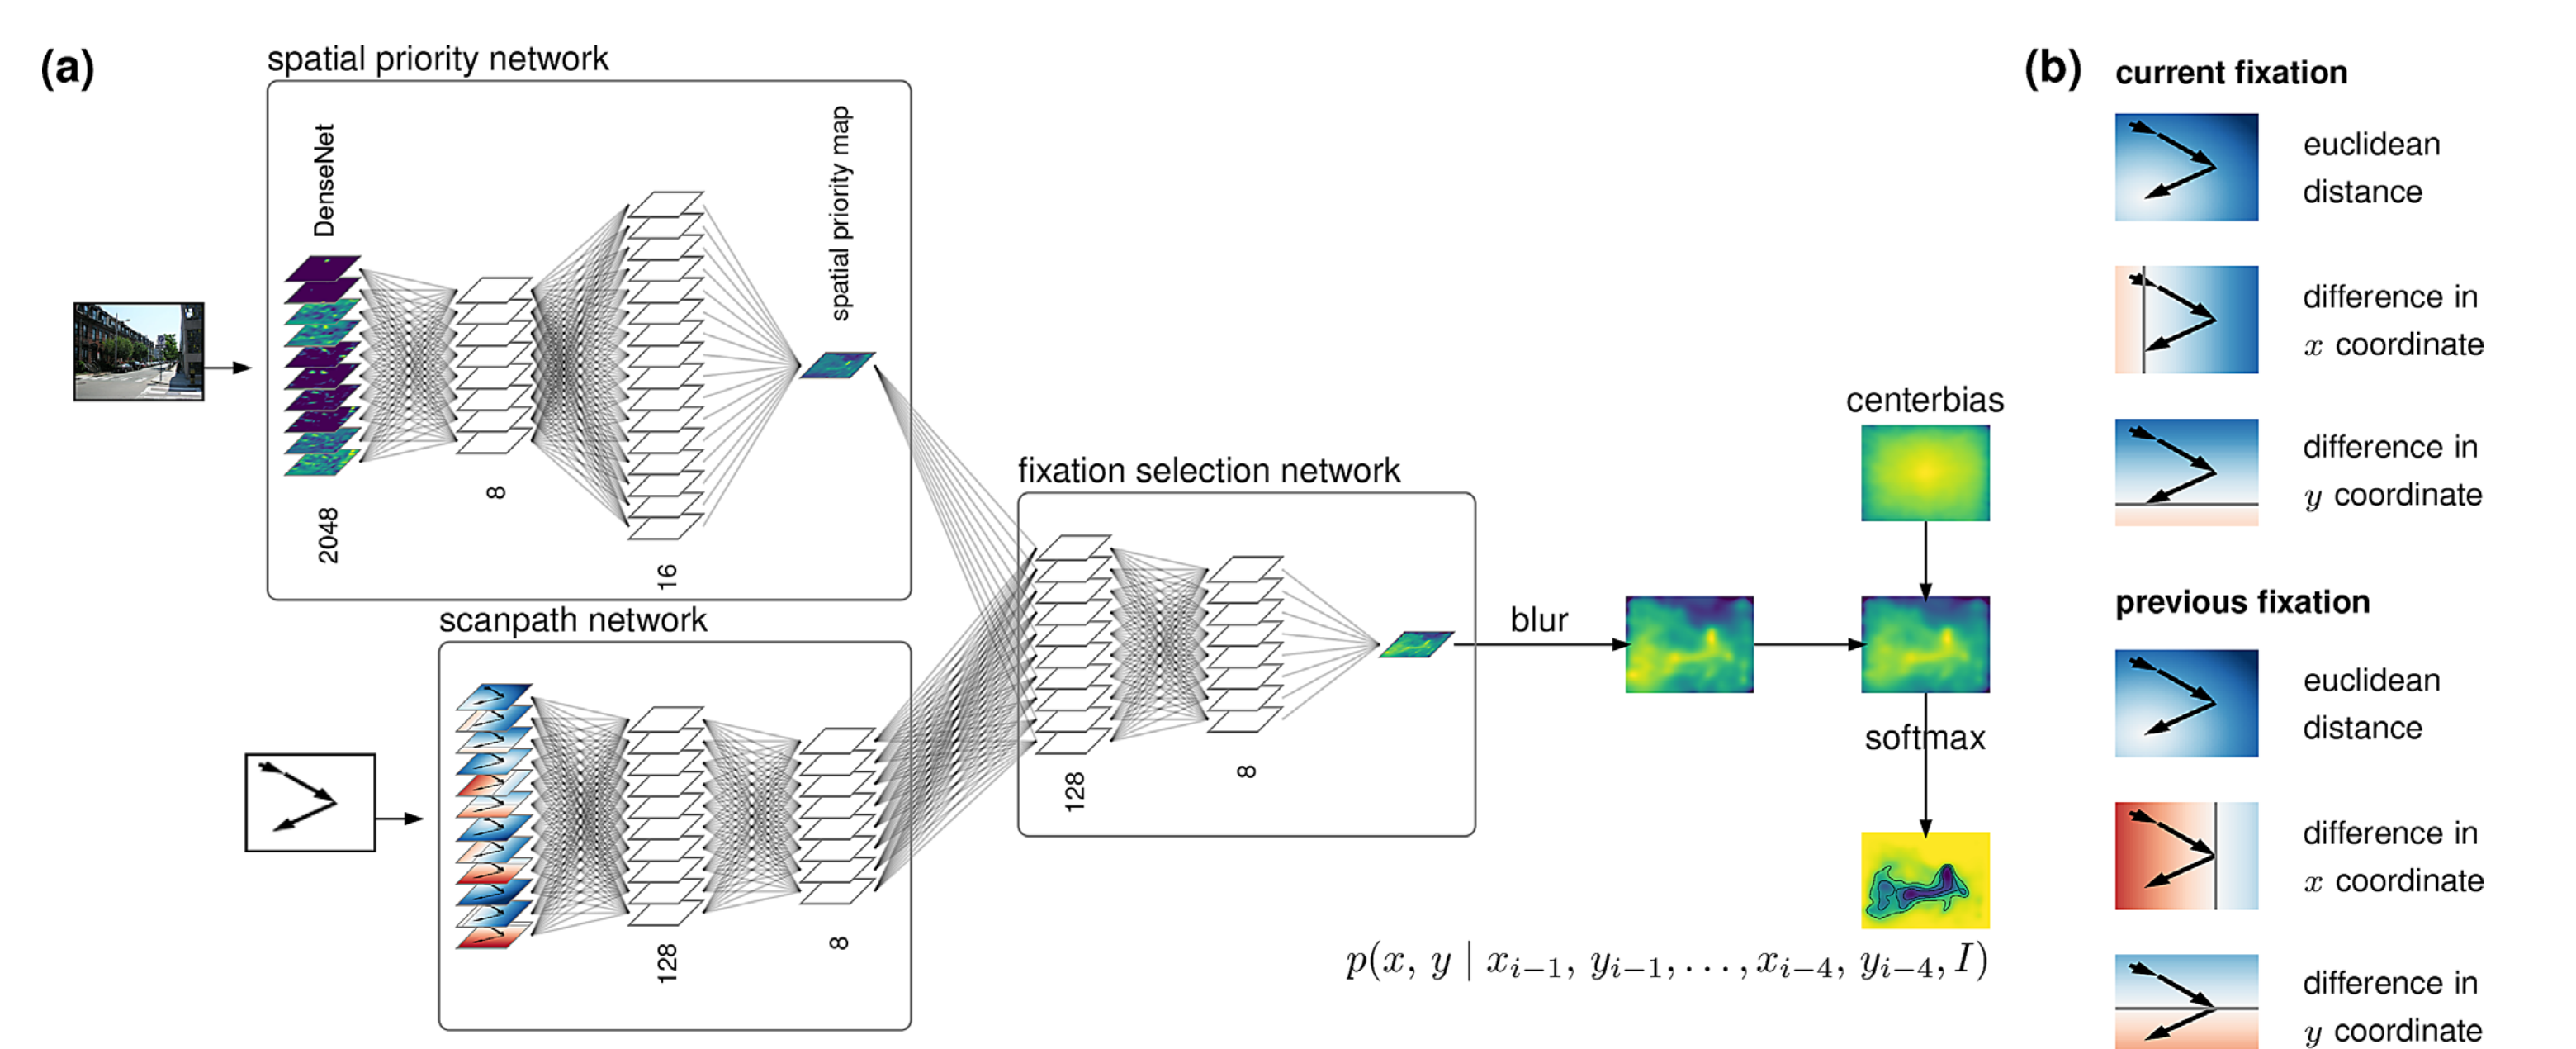
\includegraphics[width=0.99\textwidth]{kummerer2022_dg3_fig2.png}};
    \begin{scope}[x={(dgimg.south east)}, y={(dgimg.north west)}]
      \node[draw, very thick, rounded corners=2pt, fill=blue!15, align=center,
            font=\scriptsize\bfseries, inner sep=2.5pt] (fov) at (0.058,0.505)
        {foveation\\ \textnormal{\itshape (this thesis)}};
      \draw[-{Latex[length=2.2mm]}, very thick, blue!55!black] (fov.north) -- (0.058,0.625);
    \end{scope}
  \end{tikzpicture}
  \caption[\dg{}'s forward pass, with the foveation marked]{\dg{}'s forward pass. \textbf{(a)} The shaded box marks the input foveation of
    \secref{foveation}; everything after it is the published model. \textbf{(b)} The three maps each
    of the last four fixations becomes (two of the four drawn). \emph{Panels adapted from
    \citet{kummerer2022deepgaze3}, Figure~2.}}
  \label{fig:dg3-published}
\end{figure}

\begin{figure}[tbp]
  \centering
  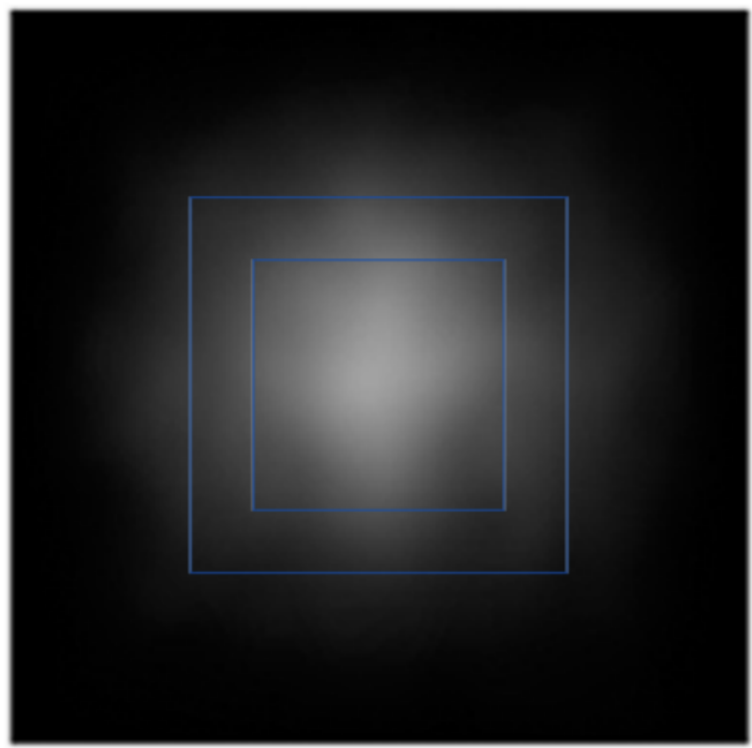
\includegraphics[width=0.44\textwidth]{judd2009_meanfixations.png}
  \caption[The MIT1003 centerbias]{All human fixations averaged over the 1003 MIT1003 images. The inner
    box covers the central $11\%$ of the image area and contains $40\%$ of all fixations, the outer box
    $25\%$ and $70\%$. Reproduced from \citet{judd2009mit1003}.}
  \label{fig:judd-centerbias}
\end{figure}

The foveation attaches before the backbone. The image is foveated, and everything downstream runs
unchanged. The comparison is clean because only the read-out carries trainable weights. Retraining under
a changed input (\secref{training}) adapts nothing else, so a measured difference is attributable to the
input rather than to a re-tuned backbone.

\section{Dataset and evaluation framework}
\label{sec:eval-framework}

Every quantitative result in this thesis comes from one evaluator, one dataset, and one fixed partition
of that dataset.

\subsection{The MIT1003 free-viewing dataset}
\label{subsec:mit1003}

The dataset used throughout is MIT1003 \citep{judd2009mit1003}. Its 1003 natural images were each freely
viewed for three seconds by up to fifteen subjects while eye position was recorded.

MIT1003 keeps each subject's scanpath separate and in viewing order, which the multi-subject analyses
of \secref{multi-subject} need.
It is also the dataset \dg{} was trained and benchmarked on \citep{kummerer2022deepgaze3}, so the
pretrained model is evaluated on the images it was fitted to.

The dataset is accessed through the \texttt{pysaliency} library (Appendix~\ref{app:data}).
Successive images were separated by one second of a gray screen, and every recorded scanpath begins with
a fixation at the image centre. \citet{judd2009mit1003} discard that initial centre fixation as trivial;
the variant loaded here keeps it, following the published \dg{} evaluation
\citep{kummerer2022deepgaze3}.
The centre fixation serves as history only, never as a target, and every free fixation is scored, which
gives $104{,}171$ fixations and puts the baseline on the protocol of the published figure.
Every arm is trained and scored under this protocol.

\subsection{Image-stratified cross-validation}
\label{subsec:cv-split}

The dataset is partitioned into ten folds of about $100$ images each. Every scanpath of an image
lands in the same fold, so a test image is never seen during training.
Each split takes eight folds for training, one for validation, and one for test
(Appendix~\ref{app:data}). The folds come from \texttt{pysaliency}'s cross-validation splitter, whose
fixed internal seed reproduces the partition the published \dg{} training notebook used
\citep{deepgazepytorch}.
Every arm of \secref{training} is trained ten times, once per fold, so an arm is ten models
(\figref{cv-split}).

\begin{figure}[tbp]
  \centering
  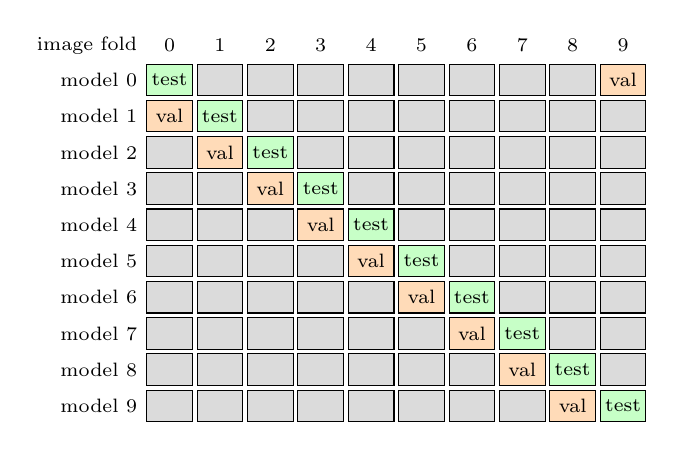
\begin{tikzpicture}[x=6.4mm, y=4.6mm, font=\scriptsize]
    \foreach \i in {0,...,9} { \node at (\i, 0.95) {\i}; }
    \node[anchor=east, font=\scriptsize] at (-0.45, 0.95) {image fold};
    \foreach \k in {0,...,9} {
      \node[anchor=east] at (-0.45, -\k) {model \k};
      \foreach \i in {0,...,9} {
        \pgfmathtruncatemacro{\isT}{ifthenelse(\i==\k,1,0)}
        \pgfmathtruncatemacro{\vv}{mod(\k+9,10)}
        \pgfmathtruncatemacro{\isV}{ifthenelse(\i==\vv,1,0)}
        \ifnum\isT=1
          \node[draw, fill=green!22, minimum width=5.8mm, minimum height=4.0mm, inner sep=0pt]
            at (\i,-\k) {test};
        \else
          \ifnum\isV=1
            \node[draw, fill=orange!28, minimum width=5.8mm, minimum height=4.0mm, inner sep=0pt]
              at (\i,-\k) {val};
          \else
            \node[draw, fill=black!14, minimum width=5.8mm, minimum height=4.0mm, inner sep=0pt]
              at (\i,-\k) {};
          \fi
        \fi
      }
    }
  \end{tikzpicture}
  \caption[The ten-fold image-stratified partition]{Each row is one of the ten models an arm consists of; every image is the test image of exactly
    one, so the ten test evaluations together cover the dataset once.}
  \label{fig:cv-split}
\end{figure}

The learning rate and the epoch the comparison is read at are chosen on the validation fold, and every
check that training behaved runs there. The test fold is scored after all training is complete, and it
is the source of the arm comparison in \chref{results}.

\subsection{Distribution-level performance metrics}
\label{subsec:metrics}

\dg{} outputs a probability map, the probability at each pixel that the next fixation lands there
(\secref{dg3-arch}).
All metrics are computed by reading this map at the pixel nearest each human fixation, never by comparing
scanpaths sampled from the model with human ones (\secref{models}; \citealp{kummerer2021state}).

Four metrics are computed per fixation, averaged per image and then over the images of a fold:
information gain, log-likelihood, NSS and AUC. Information gain is the primary one.
Throughout, an image has $H$ rows and $W$ columns, so $HW$ is its pixel count; $p(\vect{x})$ is the
probability the map puts on pixel $\vect{x}$; and $\vect{x}_1, \ldots, \vect{x}_n$ are the $n$ pixels
subjects were recorded fixating.

The \emph{log-likelihood} asks how much more probability the model put on those pixels than a map giving
every pixel the same value, $1/HW$. It is reported in \emph{bits per fixation}, where each bit doubles
the probability the model gave the pixel the subject chose, relative to a uniform map.

\begin{equation}
  \LL = \frac{1}{n} \sum_{i=1}^{n} \log_2 \frac{p(\vect{x}_i)}{1/HW}.
  \label{eq:ll}
\end{equation}

A uniform map is a weak reference, because free-viewing gaze concentrates near the image centre whatever
the picture shows. \emph{Information gain} is the same measurement with the reference swapped for the
centerbias, the prior that already knows about that tendency, so what remains is the information the
model adds beyond it \citep{kummerer2015information, kummerer2018benchmarking}:

\begin{equation}
  \IG = \LL_\text{model} - \LL_\text{centerbias},
  \label{eq:ig}
\end{equation}

also in bits per fixation, and zero for a model that adds nothing to the prior.
This is the measure \citet{kummerer2022deepgaze3} report for \dg{}.
The centerbias used here is the one distributed with the \dg{} release \citep{deepgazepytorch}, the same
prior the Finalizer adds (\secref{dg3-arch}), resized to each stimulus (Appendix~\ref{app:eval}).
\figref{scanpath-density} shows the maps \eqnref{ig} is read from along one scanpath, under the sharp
control and one foveated arm.

\begin{figure}[tbp]
  \centering
  \includegraphics[width=\textwidth, height=0.86\textheight, keepaspectratio]%
    {foveation_mit1003_initial/figs/scanpath_density_fov_cpd20_stim0091.png}
  \caption[One scanpath scored step by step]{The first five steps of one subject's scanpath on a held-out stimulus. The input column is the
    frame the foveated arm receives, re-centred on the current fixation (circle), with the subject's
    next saccade (arrow and star); each map is read at the pixel the subject moved to next, and
    averaging those terms over every scanpath in a fold is what the evaluator reports. The history is
    the subject's own fixations, never a path the model drew.}
  \label{fig:scanpath-density}
\end{figure}

NSS and AUC are not in bits and are reported alongside.
The normalised scanpath saliency \citep{peters2005nss},

\begin{equation}
  \NSS = \frac{1}{n} \sum_{i=1}^{n} \frac{p(\vect{x}_i) - \mu_p}{\sigma_p},
  \label{eq:nss}
\end{equation}

rescales the map to zero mean and unit standard deviation over its pixels ($\mu_p$ and $\sigma_p$) and
reads it where people looked, so it measures how much the model rated those places above its own
average.
The area-under-curve (AUC) metric asks a ranking question instead. Take a pixel someone fixated and a
pixel drawn at random from the same image; AUC is the probability the model rated the fixated one
higher:

\begin{equation}
  \AUC = \frac{1}{n\,HW} \sum_{i=1}^{n} \sum_{u=1}^{HW}
    \Big(\mathbf{1}\big[p(\vect{x}_i) > p_u\big]
       + \tfrac{1}{2}\,\mathbf{1}\big[p(\vect{x}_i) = p_u\big]\Big),
  \label{eq:auc}
\end{equation}

where the inner sum runs over every pixel $p_u$ of the image and $\mathbf{1}[\cdot]$ is the indicator
function, $1$ when the condition inside holds and $0$ otherwise. The discretised density makes exact
ties common, so they count half.
Only the order of the values matters, so AUC is unchanged by any rescaling of the map that preserves
it, and measures \emph{discrimination}, where the likelihood metrics reward getting the values
themselves right as well.
The shuffled-AUC variant is not used, because it draws its random pixels from other images' fixations
rather than uniformly, which divides the centerbias out \citep{kummerer2018benchmarking}, and that prior is
what \eqnref{ig} already measures against.

\section{Human variability and per-image difficulty}
\label{sec:multi-subject}
\label{subsec:difficulty-proxies}

Model fit varies widely between images, and the question here is what makes an image easy or hard. Human
agreement is the candidate, so the spread of the fifteen scanpaths has to be measured before it can be
correlated with anything.

The normalised Shannon entropy $H_{\text{fix}}$ of the population fixation density follows
\citet{judd2009mit1003}, who score per-image consistency as the entropy of the human fixation map pooled
over subjects; the version here bins the fixations rather than smoothing them.
All subjects' free fixations are pooled, binned into a $16 \times 16$ grid, and normalised to a probability
mass $p_k$ over the $K = 256$ cells,

\begin{equation}
  H_{\text{fix}} \;=\; -\frac{1}{\log_2 K} \sum_{k=1}^{K} p_k \log_2 p_k,
  \label{eq:fix-entropy}
\end{equation}

with $\log_2 K = 8$ putting $H_{\text{fix}}$ in $[0, 1]$. It rises as the population's gaze spreads.
\figref{entropy-panel} shows the quantity on the dataset's two extremes.

\begin{figure}[tbp]
  \centering
  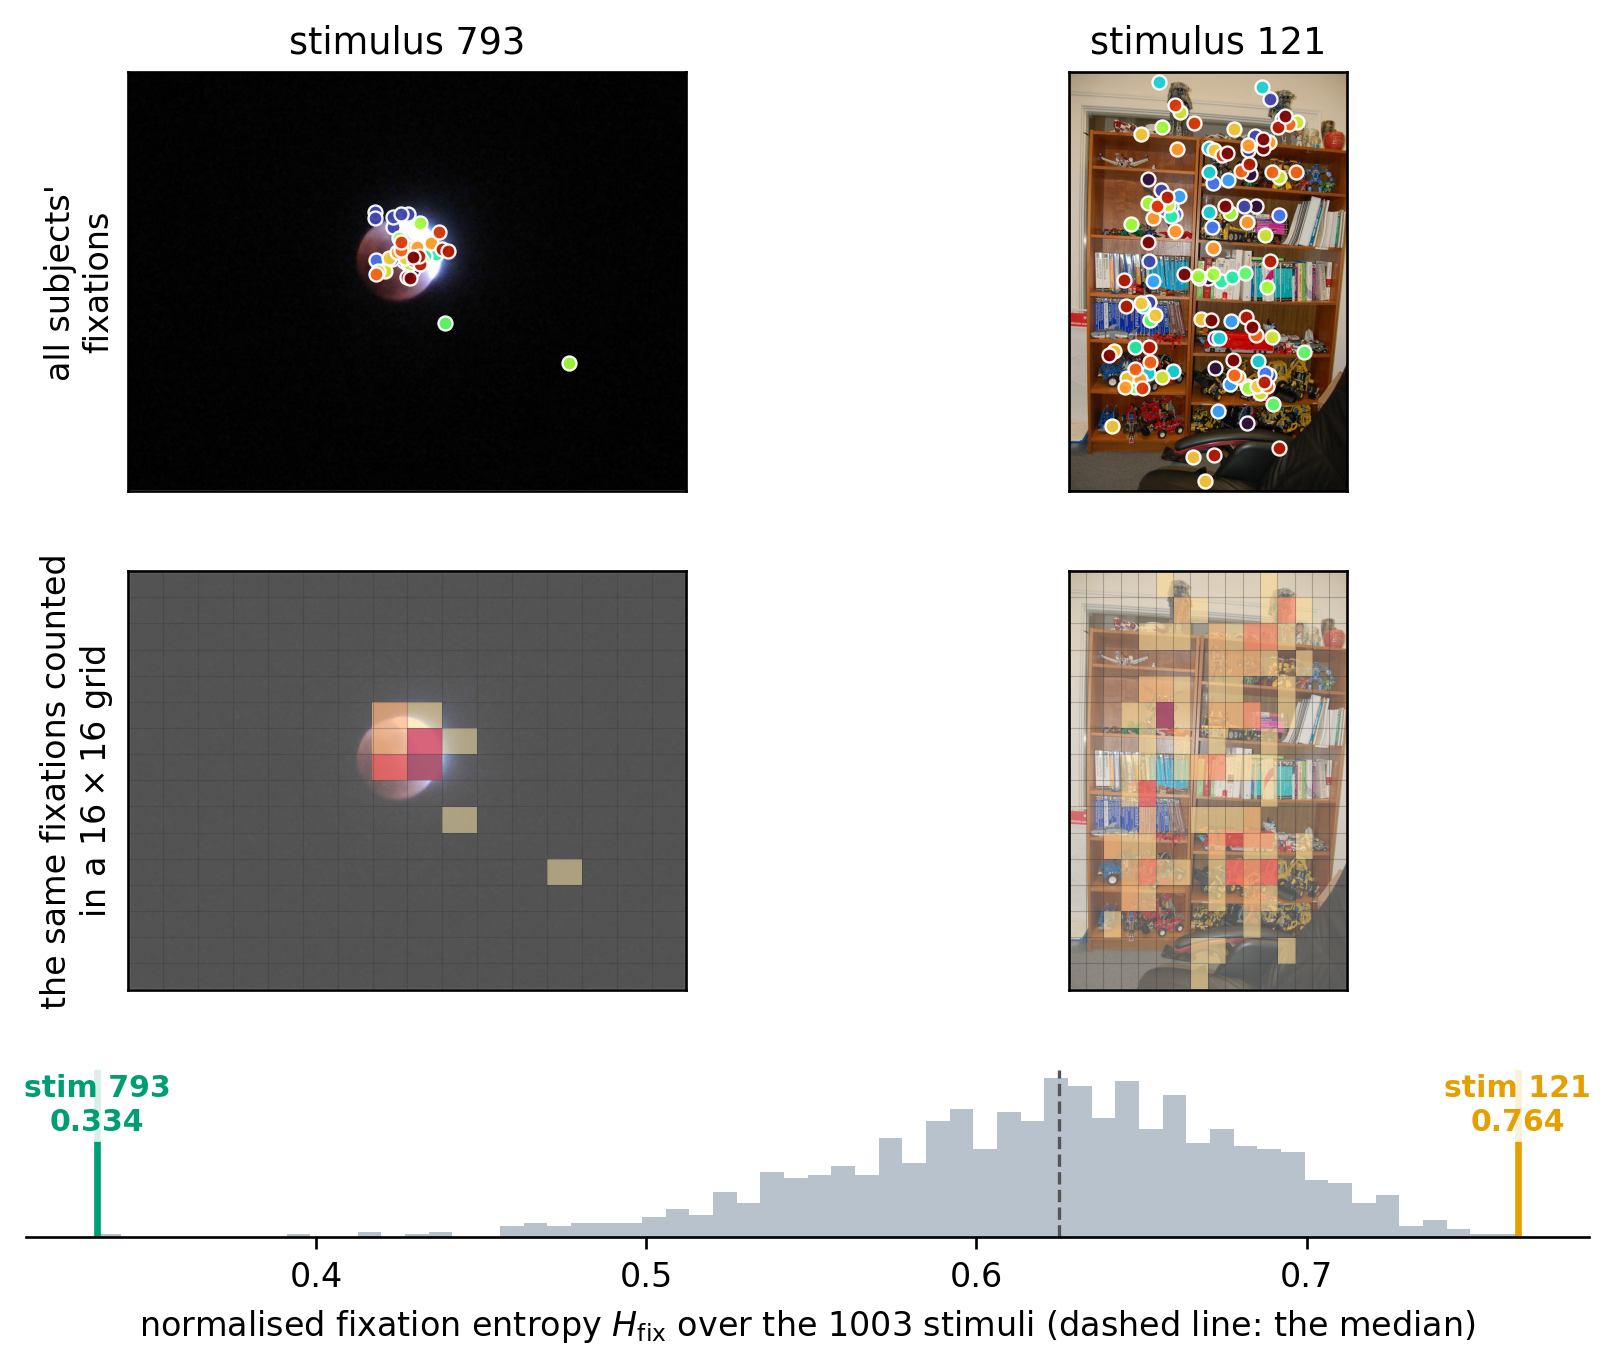
\includegraphics[width=\textwidth]{foveation_mit1003_initial/figs/entropy_panel.png}
  \caption[Fixation entropy at the dataset's extremes]{The stimulus where the subjects agreed most and the one where they agreed least, with their
    fixations, the same fixations counted into the $16 \times 16$ grid of \eqnref{fix-entropy}, and
    where both sit on the distribution over the 1003 stimuli.}
  \label{fig:entropy-panel}
\end{figure}

$H_{\text{fix}}$ is correlated against per-image model performance in \chref{results}. There the four
metrics of \subsecref{metrics} are computed per image, pooling only the subjects who viewed it. Both
Pearson's $r$ and Spearman's rank $\rho$ are reported.

\section{Gaze-contingent input foveation}
\label{sec:foveation}

\chref{background} introduced the acuity model; this section defines the transformation built on it:
the parametrised blur (\subsecref{gp-model}) and what its one strength parameter means against the
display and the dataset's saccades (\subsecref{sharp-radius}).
The fovea is re-centred on the most recent fixation of the history before every forward pass, in
training and in evaluation, so the foveation is \emph{gaze-contingent} and each pass sees the image as
a subject fixating there would.

\subsection{The blur and its parameters}
\label{subsec:gp-model}

The falloff is specified in degrees of visual angle, so its strength can be compared against measured
human acuity and carried unchanged across screen geometries.
Following \citet{geislerperry1998}, the highest spatial frequency resolvable at eccentricity $e$ (in
degrees) falls as

\begin{equation}
  f_c(e) \;=\; f_{c0}\,\frac{e_2}{e + e_2} \qquad [\text{cyc/deg}],
  \label{eq:gp-acuity}
\end{equation}

with foveal cutoff $f_{c0}$ and the half-acuity eccentricity fixed at $e_2 = 2.3^\circ$ in
\secref{foveated-vision}.
Their fitted contrast-threshold law puts the foveal cutoff at 39--41~cyc/deg
(Appendix~\ref{app:foveation}), so this work takes $f_{c0} = 40$~cyc/deg as the human setting.

$\ppd$ is how many pixels fit into one degree of visual angle on the subject's screen, set by screen
size, resolution, and viewing distance; for MIT1003, $\ppd = 35$ (Appendix~\ref{app:foveation}).
Dividing a pixel distance by $\ppd$ converts it to the degrees \eqnref{gp-acuity} expects,
$e_{\text{deg}} = e_{\text{px}} / \ppd$.

The naive way to apply the falloff is one blur per pixel. The image is foveated instead by blending a
Gaussian pyramid, a stack of uniformly-blurred copies built once per image, starting from the sharp
original and doubling the blur at each level. Every pixel is a linear interpolation between two levels,
so an image is blurred a few times instead of several hundred thousand.
The \emph{Nyquist} frequency is the highest frequency the display can carry, half its sampling rate,
here $0.5$~cyc/px.
For each pixel the target cutoff $f_c(e)$ of \eqnref{gp-acuity} is converted to cycles-per-pixel and
clamped at that limit; the corresponding fractional pyramid level is

\begin{equation}
  L(e) \;=\; \log_2\!\frac{0.5}{f_{c,\text{px}}(e)},
  \label{eq:frac-level}
\end{equation}

zero at the fovea and growing with eccentricity.
The foveated pixel is a linear interpolation between the two integer levels bracketing $L(e)$.
\figref{gp-pyramid} shows the construction; implementation detail is in Appendix~\ref{app:foveation}.

\begin{figure}[tbp]
  \centering
  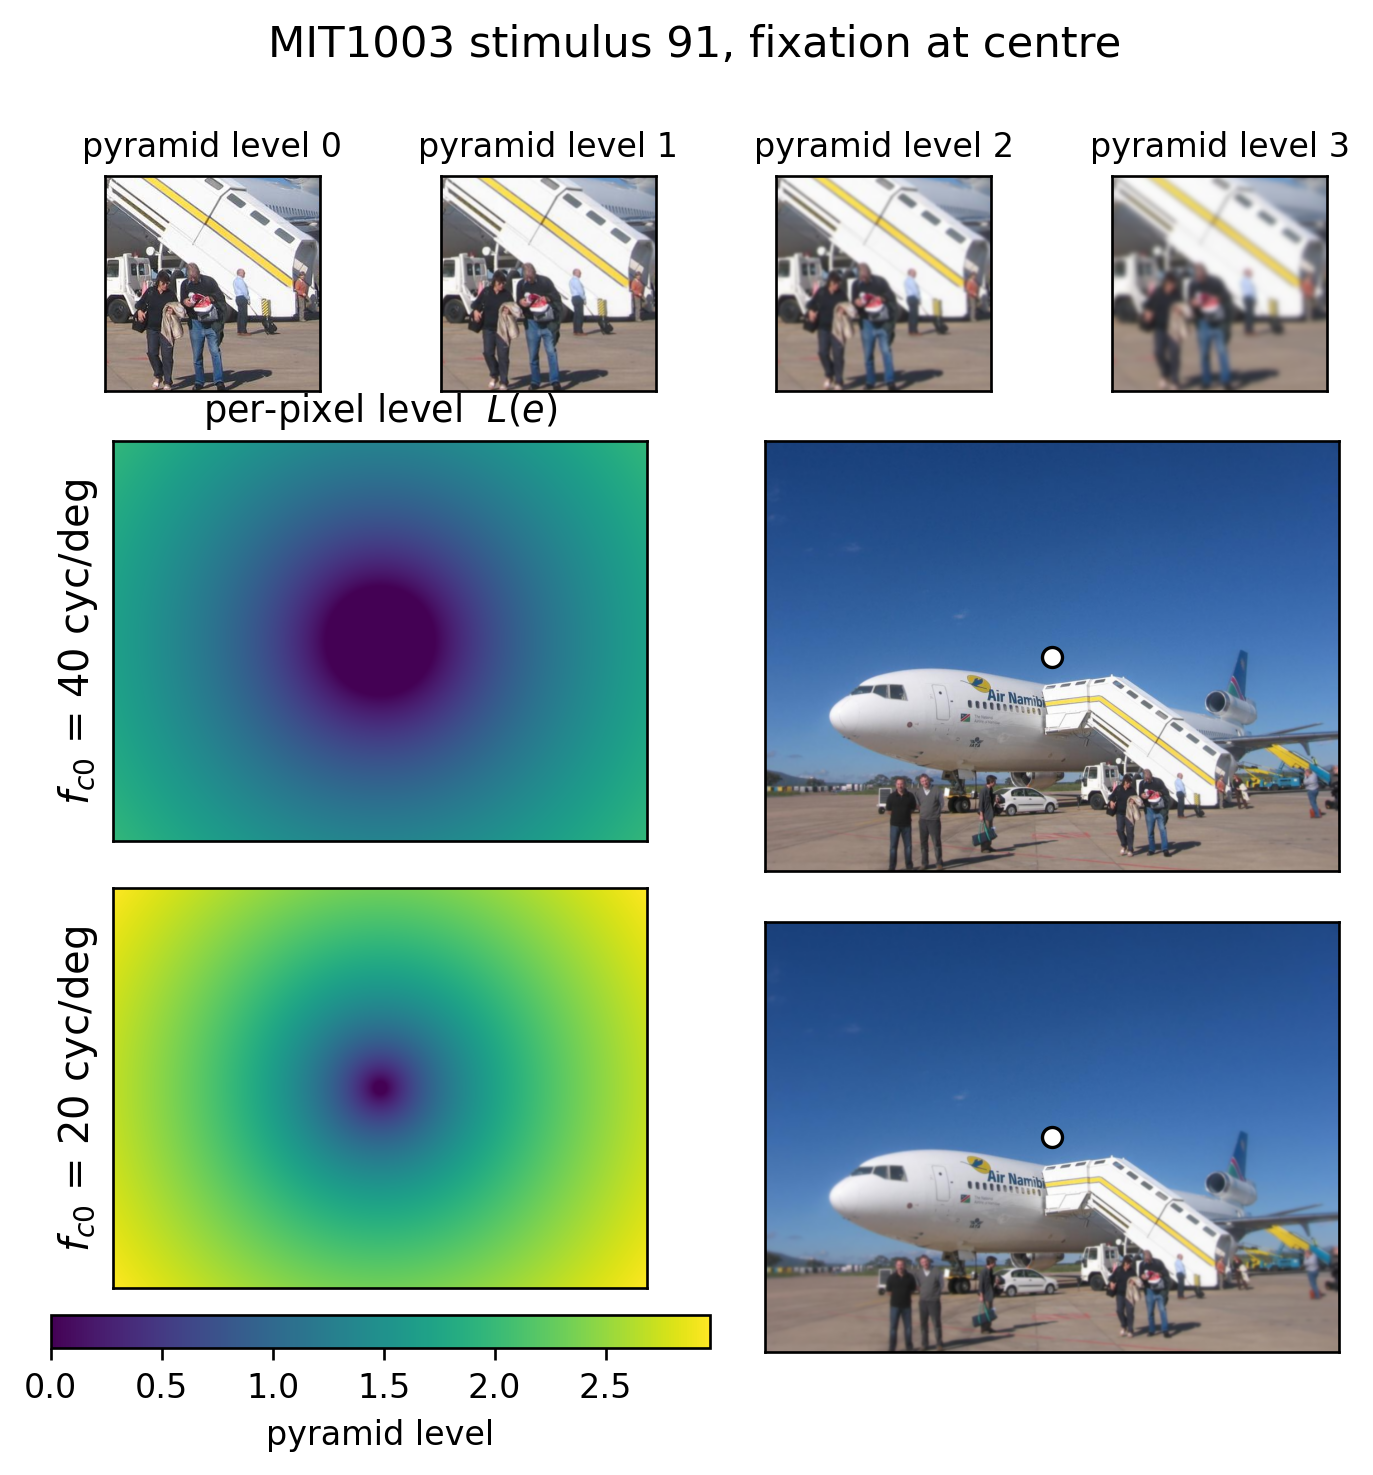
\includegraphics[width=\textwidth]{foveation_mit1003/figs/gp_pyramid.png}
  \caption[How the space-variant blur is built]{Top: the four shallowest pyramid levels on one patch, magnified because at full-frame size they
    are indistinguishable. Below, for each cutoff: the per-pixel level $L(e)$ of \eqnref{frac-level},
    dark where the frame stays sharp, and the foveated frame it produces.}
  \label{fig:gp-pyramid}
\end{figure}

The acuity profile forces one deviation from the published \dg{} protocol.
\citet{kummerer2022deepgaze3} resize every MIT1003 stimulus to $768 \times 1024$ or $1024 \times 768$.
Since the longest side is already $1024$~px, only the short axis stretches, and a stretched image turns
the sharp region around gaze into an ellipse rather than a disc.
This work therefore trains and evaluates at native resolution.
The released checkpoint was fitted on the resized stimuli, so native input is a mild distribution shift
for it.

\subsection{The sharp radius}
\label{subsec:sharp-radius}

At the MIT1003 geometry the Nyquist limit is $0.5\,\ppd = 17.5$~cyc/deg, and it is a property of the
display, so it is the same at every eccentricity.
Wherever $f_c(e)$ is above it the eye out-resolves the display, the clamp in \eqnref{frac-level} holds
$L$ at zero, and those pixels stay bit-identical to the sharp input; the fovea is therefore equally
sharp at every cutoff above the limit, and $f_{c0}$ controls how far out the sharp region reaches. At
$f_{c0} = 10$ the curve starts below the limit, so even the fovea is blurred.
Solving \eqnref{gp-acuity} for the eccentricity at which $f_c(e)$ meets the limit gives that radius in
closed form:

\begin{equation}
  e_{\text{sharp}} \;=\; e_2\!\left(\frac{2 f_{c0}}{\ppd} - 1\right) \quad [\text{degrees}]
  \quad\Longrightarrow\quad
  \ppd \cdot e_{\text{sharp}} \;=\; e_2\,(2 f_{c0} - \ppd) \quad [\text{pixels}].
  \label{eq:sharp-radius}
\end{equation}

At $f_{c0} = 40$ the sharp disc reaches $3.0^\circ$, while an MIT1003 stimulus spans
$29^\circ$ along its long side at $\ppd = 35$, so most of the frame is blurred at every cutoff.
Foveation strength is set by $f_{c0}$, with lower cutoffs blurring more.
\figref{foveation-strength} plots both sides of \eqnref{sharp-radius}, the crossing it solves and
the disc that crossing leaves on the frame.

\begin{figure}[tbp]
  \centering
  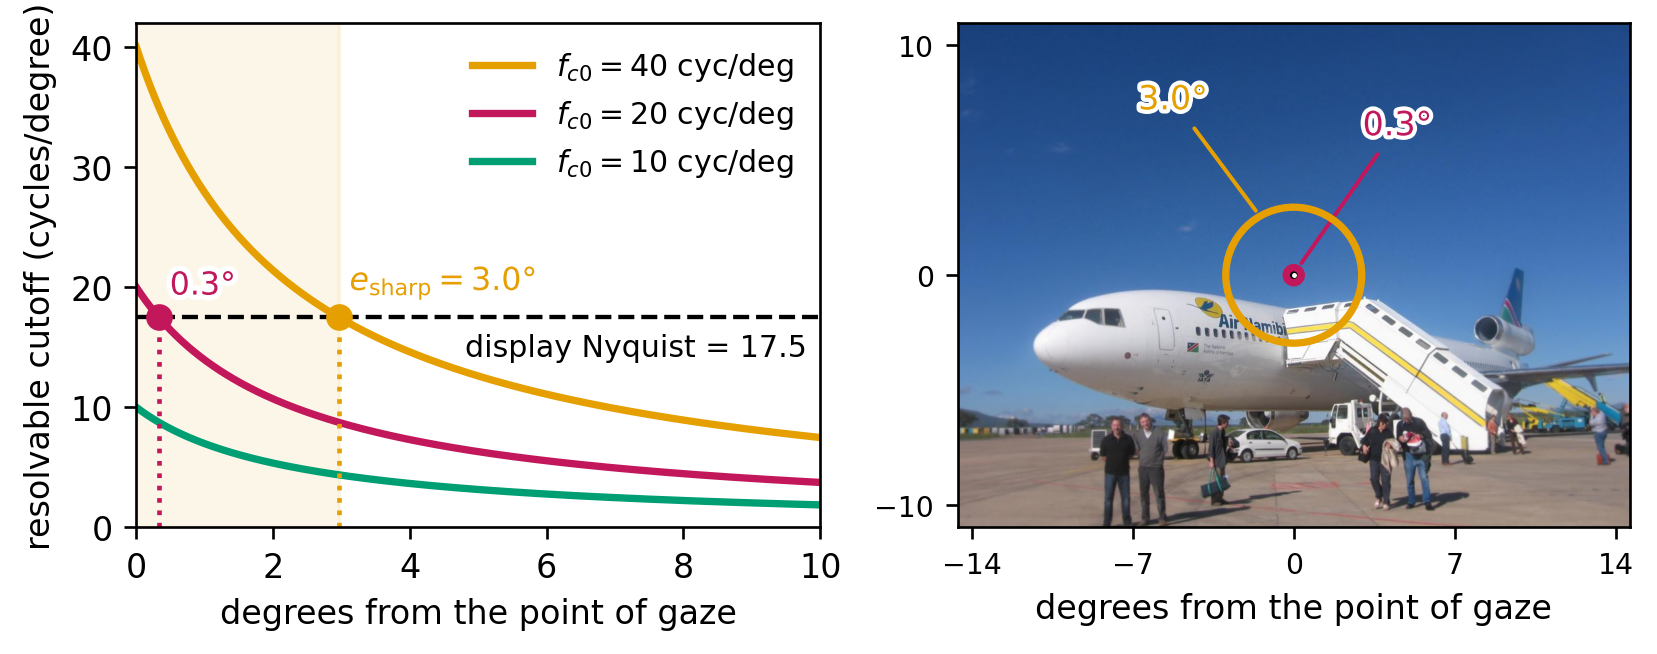
\includegraphics[width=0.98\textwidth]{foveation_mit1003/figs/foveation_strength.png}
  \caption[The sharp radius]{The sharp radius at the three cutoffs of the arm list. Left: the falloff of \eqnref{gp-acuity}
    against the display Nyquist limit, with the crossing of \eqnref{sharp-radius} carried down to
    the axis; at $f_{c0} = 10$ the curve starts below the line, so that arm has no sharp disc. Right:
    the two remaining radii on stimulus~91, foveated at $f_{c0} = 40$ with the fovea at the image
    centre.}
  \label{fig:foveation-strength}
\end{figure}

The sharp disc reaches further than the fovea's $2^\circ$ (\secref{foveated-vision}) and than the
$e_2 = 2.3^\circ$ at which the eye's cutoff has halved, because the MIT1003 display carries only
$17.5$~cyc/deg and the eye does not fall to that until $3.0^\circ$. Out to that eccentricity a subject
out-resolves the screen, so blurring the image down to what the eye could see removes nothing that was
displayed. Given the acuity model, the sharp disc therefore follows from the display rather than from a
free parameter.

The sharp radius ties the strength sweep to the saccades the evaluator scores. Every scored
transition is a human saccade (\subsecref{metrics}), with a median amplitude of $155$~px ($4.4^\circ$
at $\ppd = 35$) over all $104{,}171$ of them, and \figref{saccade-coverage} reports for each cutoff the
fraction whose target falls inside the sharp disc and so reaches the backbone at full resolution:
$32.9\%$ at $f_{c0} = 40$, $0.6\%$ at $20$, and effectively none at $10$, where the disc has closed.

\begin{figure}[tbp]
  \centering
  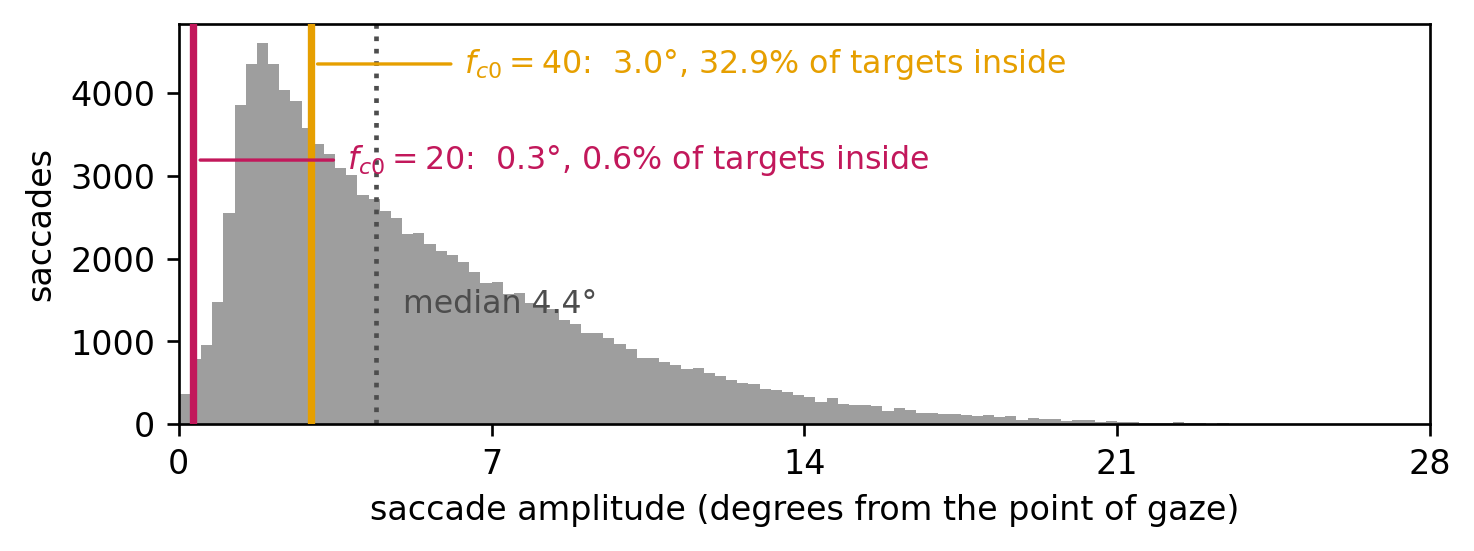
\includegraphics[width=0.94\textwidth]{foveation_mit1003/figs/saccade_coverage.png}
  \caption[Saccade amplitudes against the sharp radii]{The amplitudes of the $104{,}171$ saccades the
    evaluator scores, with the sharp radius of \eqnref{sharp-radius} marked for the two cutoffs that
    have one.}
  \label{fig:saccade-coverage}
\end{figure}

Between $40$ and $20$ the sharp disc shrinks past the typical saccade, so targets stop being delivered
sharp; between $20$ and $10$ almost no target is sharp in either arm, and any further cost comes
from how severely the target is blurred.
\figref{gp-strength} shows the strengths on four images, and the input column of
\figref{scanpath-density} the fovea moving down a subject's scanpath.

\begin{figure}[tbp]
  \centering
  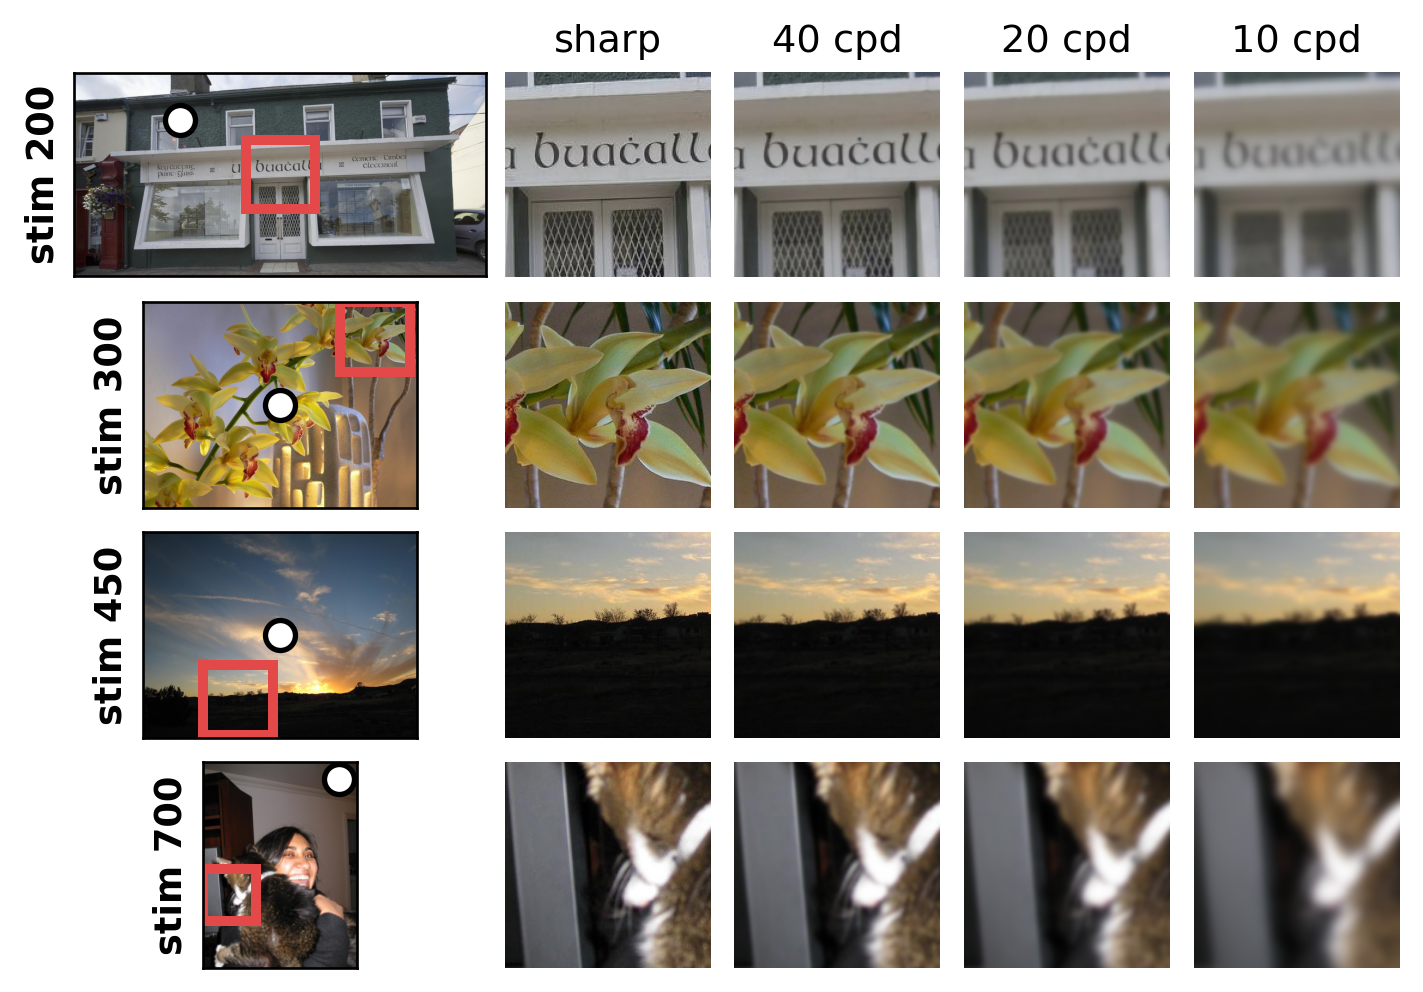
\includegraphics[width=\textwidth]{foveation_mit1003/figs/gp_strength_grid.png}
  \caption[Foveation strength on four stimuli]{Four MIT1003 images with the fovea held at the white dot, and the marked patch enlarged at each
    strength. Averaged over the four, the mean absolute change from the sharp original is $1.8/255$
    at $f_{c0} = 40$ and $5.6/255$ at $f_{c0} = 10$. The trained model re-centres the fovea on every
    fixation; it is held still here only to show strength.}
  \label{fig:gp-strength}
\end{figure}

\section{Training protocol: read-out fine-tuning on sharp versus foveated input}
\label{sec:training}

Networks fitted to sharp images lose accuracy under blur \citep{hendrycks2019robustness}, so \dg{} with
its pretrained read-out should be expected to underperform on foveated input. That penalty
measures the unfamiliarity of blurred input rather than what the removed detail was worth, so each arm
fine-tunes the read-out on its own input and the arms are compared after adaptation.
\subsecref{results-arms} reports what that penalty is before any fine-tuning.

\subsection{The arms}
\label{subsec:arms}

Every arm starts from pretrained \dg{} with the backbone and the Finalizer frozen (\secref{dg3-arch}),
and an audit asserts at construction that exactly the read-out is trainable (Appendix~\ref{app:training}).
The pretrained read-out is the released mixture of ten (\secref{dg3-arch}), each fitted on eight of these
same folds, and all ten are fine-tuned together, so a fold's test images were training data for most of
the read-outs its arms start from. Every arm shares that start, so the differences between arms are
unaffected; the absolute levels in \chref{results} are partly in-sample and sit above the published
cross-validated figure.

The cutoff $f_{c0}$ is swept from human acuity at $40$ down to $20$ and $10$~cyc/deg. One strength on
its own cannot separate a foveation that costs nothing from one too mild to measure, while a real cost
deepens as the periphery is degraded. Blur alone could produce such a cost, since the backbone was
pretrained on sharp photographs. Each cutoff therefore has a fixed-centre twin carrying the identical
blur pinned to the image centre, so the pair differs only in whether the sharp region follows the gaze.
With the sharp control, that makes the seven arms of \tabref{arms}.

Every arm is trained on all ten folds and shares the protocol (data, folds, optimiser, learning-rate
schedule, epoch count, seed, and the nearest-pixel target convention below), so the arms differ in
nothing but the input (Appendix~\ref{app:training}).

\begin{table}[tbp]
  \centering
  \caption[The seven arms]{The seven arms; only the input differs between them, and the sharp arm is the
    control every difference is taken against. The sharp radius sets what each cutoff is for
    (\subsecref{sharp-radius}): $f_{c0} = 40$ is human acuity and the main comparison, $20$ sits
    past the point where the sharp disc still covers a typical saccade, and $10$ is a coarse probe.}
  \label{tab:arms}
  \small
  \begin{tabular}{lcc}
    \toprule
    arm & fovea & $f_{c0}$ (cyc/deg) \\
    \midrule
    sharp (control)   & ---                          & --- \\
    \addlinespace[2pt]
    gaze-contingent   & follows the current fixation & $40$, $20$, $10$ \\
    \addlinespace[2pt]
    fixed-centre      & image centre                 & $40$, $20$, $10$ \\
    \bottomrule
  \end{tabular}
\end{table}

\subsection{Loss and optimisation}
\label{subsec:training-loop}

One training example is a \emph{(history, target) pair}, up to four fixations preceding some moment in one
subject's scanpath on one image and the location that subject moved to next.
The objective is the negative log-probability the model assigns to that location, identical to
\eqnref{ll} up to sign, base and a constant.
For a training image with $N_f$ such pairs, pooled across all subjects who viewed it,

\begin{equation}
  \mathcal{L}(\theta; \text{image})
  \;=\;
  -\frac{1}{N_f} \sum_{j=1}^{N_f} \log p_{\theta}(\vect{t}_j \mid \mathcal{H}_j, \text{image}),
  \label{eq:training-loss}
\end{equation}

with $\theta$ the trainable read-out parameters. The earliest pair of each scanpath predicts the first
free fixation from the centre fixation, as in the evaluator (\subsecref{mit1003}).
The target log-density is read at the pixel nearest $\vect{t}_j$, the same nearest-pixel lookup as in
evaluation (\subsecref{metrics}).

Optimisation is Adam over the read-out parameters, with the per-image loss accumulated in micro-batches
(Appendix~\ref{app:training}).
Each arm is trained for seven epochs at a base learning rate of $3 \times 10^{-4}$, divided by ten at
epoch five, the decaying schedule shape the \dg{} authors use.
The rate was chosen on validation and is shared by all seven arms, so
per-arm tuning cannot decide the comparison.

Epoch five is the highest in every arm, so it is the reporting epoch throughout and no per-arm choice
enters the comparison. It is also the first epoch after the decay, and epochs six and seven are run to
show that the curve flattens there rather than peaking, mean validation information gain changing by
less than $0.001$~bits per epoch across them in every arm (\figref{training-curves}).

Training runs on the Goethe-NHR cluster (Appendix~\ref{app:cluster}); the checkpoint format and gradient
clipping are in Appendix~\ref{app:training}.

\begin{figure}[tbp]
  \centering
  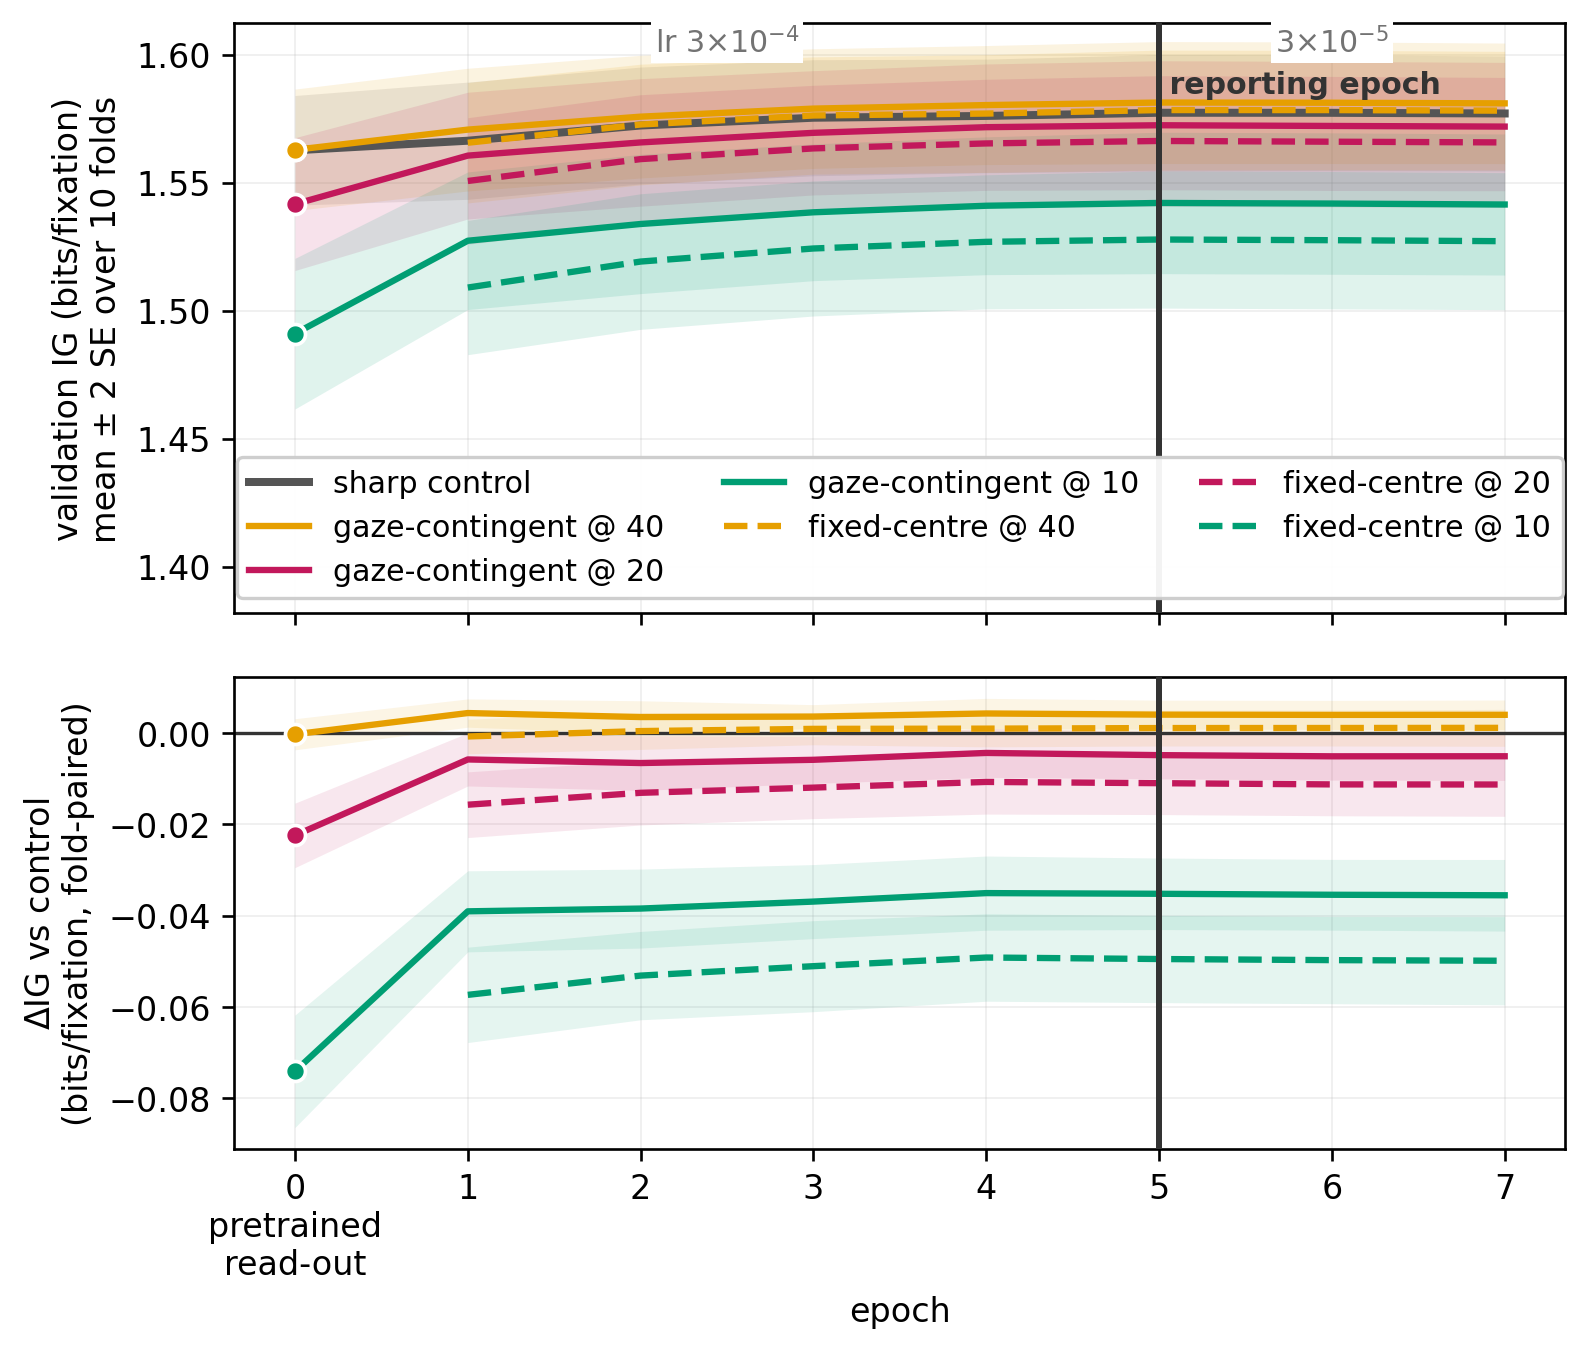
\includegraphics[width=\textwidth]{foveation_mit1003_initial/figs/training_curves.png}
  \caption[Validation curves for the seven arms]{Top: validation information gain per epoch for the seven arms. The vertical line is the reporting
    epoch, the first trained at the decayed learning rate; the dashed line marks the decay and the
    labels give the rate each segment was trained at. Epoch $0$ is the pretrained read-out every arm starts from, scored by the evaluator of
    \secref{eval-framework} (the fixed-centre arms were not scored there). Bottom: the six foveated
    arms as fold-paired differences from the sharp control.}
  \label{fig:training-curves}
\end{figure}

\subsection{The comparison and its statistics}
\label{subsec:stats-plan}

The reported quantity is a difference in information gain between two arms at a given foveation strength,

\begin{equation}
  \Delta \IG \;=\; \IG_\text{arm} - \IG_\text{reference},
  \label{eq:delta-ig}
\end{equation}

with $\IG$ as in \eqnref{ig}.
The main comparison is the gaze-contingent arm at human acuity, $f_{c0} = 40$, against the sharp
control. The two coarser cutoffs test whether the cost grows as the falloff steepens, as
\secref{position} predicts if the periphery is what makes the next saccade choosable. The fixed-centre
arms hold the blur constant and take the gaze-contingency away. NSS, AUC and the diagnostics below are
reported alongside information gain.

Both arms see the same held-out fixations (\subsecref{cv-split}), so every difference is taken within an
image. Images vary much more in difficulty than the two arms differ from one another, and taking the
difference inside an image removes that variation.

Fixations from one image are not independent, coming from one scene and from the same people. Counting
each as its own observation would make the standard error too small. Each fold is averaged to a single
number first, which leaves ten.

The reported quantity is the mean of those ten differences. Every $\pm$ and every error bar in
\chref{results} is two standard errors of that mean.
Each arm and fold is one training run from seed $42$, so the interval carries fold-to-fold variation and
no run-to-run variation.

A likelihood reads the density at one pixel and says nothing about the rest of the map, so two arms can
score alike while failing in opposite ways, one spreading its mass and uncertain everywhere, the other
confident and pointing at the wrong place.
The \emph{entropy} of the predicted probability map, $-\sum p \log_2 p$ over all pixels, and the
\emph{mode distance} from the predicted peak to the true fixation separate them; the mode distance is
interpretable in pixels where bits are not.
Both are computed for both arms on identical scanpath positions, so the pairing is exact, and both are
reported as fold means, like the primary difference.
The difference of \eqnref{delta-ig} is also stratified, by saccade amplitude and by fixation index,
since a foveation effect should depend on how far the eye is moving and the earliest fixations are
centre-driven.
Two of the amplitude bin edges sit at the sharp radii of \eqnref{sharp-radius} ($11.5$~px at
$f_{c0} = 20$, $103.5$~px at $f_{c0} = 40$), so each bin lies wholly inside or wholly outside an arm's
sharp disc, and whether the cost appears where the disc ends can be read straight off the binned
differences.

These diagnostics are computed on the \emph{validation} split.
The test folds are reserved for the main comparison (\subsecref{cv-split}).



\chapter{Results}
\label{ch:results}

\secref{results-foveation} reports the gaze-contingent input-foveation experiment specified in
\secref{foveation} and \secref{training}, the main experiment of this thesis, the seven arms of
\tabref{arms} over ten cross-validation folds.
\secref{results-per-image} reports the per-image diagnostic of \subsecref{difficulty-proxies}, which uses the
pretrained \dg{} read-out and characterises where the model and the human population agree.
The two sections use different read-outs on different splits, and \tabref{ledger} says which.

\begin{table}[tbp]
  \centering
  \caption[Each measurement, its read-out and its split]{Every measurement in this chapter, with the read-out it uses
    and the split it reads. The rows marked \emph{pretrained} take \dg{} as released and say nothing
    about the trained arms. Across the ten models each image is the test image exactly once and the
    validation image exactly once, so both splits span the dataset (\subsecref{cv-split}).}
  \label{tab:ledger}
  \footnotesize
  \setlength{\tabcolsep}{4pt}
  \begin{tabular}{lccc}
    \toprule
    measurement & read-out & split & sample \\
    \midrule
    Baseline (\subsecref{results-baseline})            & pretrained            & whole dataset & $104{,}171$ fixations \\
    Rate and reporting epoch (\subsecref{training-loop}) & each arm's own      & validation    & per fold \\
    Unadapted penalty (\subsecref{results-arms})       & pretrained            & validation    & $4$ arms \\
    Arm comparison (\subsecref{results-arms})          & each arm's, epoch $5$ & test          & $7$ arms \\
    Diagnostics (\subsecref{results-diagnostics})      & each arm's, epoch $5$ & validation    & $3$ contrasts \\
    Per-image variation (\secref{results-per-image})   & pretrained            & whole dataset & 1003 images \\
    \bottomrule
  \end{tabular}
\end{table}

\section{Gaze-contingent input foveation}
\label{sec:results-foveation}

\subsection{Baseline}
\label{subsec:results-baseline}

Pretrained \dg{} on the full MIT1003 dataset under the protocol of \subsecref{mit1003}
gains $1.562$~bits per fixation over the centerbias, pooled over fixations, which is
$0.026$~bits above the $1.536 \pm 0.010$ of \citet{kummerer2022deepgaze3}, Table~2. Its AUC (\eqnref{auc}) is
$0.9175 \pm 0.0018$ against their $0.916 \pm 0.001$, and its NSS
$3.265 \pm 0.066$ against their $3.257 \pm 0.016$. Both are per-image means over the 1003
stimuli.\footnote{Every $\pm$ in this chapter, and every error bar, is two standard errors of the mean
(\subsecref{stats-plan}), over the ten folds for every arm difference and over the 1003 images for the
pretrained baseline above. The values quoted from
\citet{kummerer2022deepgaze3} carry their convention rather than this one, a standard
deviation over eight repeated training runs.}
Each bit doubles the probability the model puts on the pixel a subject fixated (\subsecref{metrics}), so
$1.562$~bits is about $3$ times the probability the centerbias puts there.
This baseline is the state every arm's read-out starts from. Part of its margin over the published
figure is in-sample, since the released read-outs were fitted on these same images (\subsecref{arms});
the comparator for every difference below is the trained sharp control.

\subsection{The seven arms}
\label{subsec:results-arms}

Every arm fine-tunes its read-out on its own input, for the reason \secref{training} gives, and
everything below comes from those trained read-outs on the held-out test split.

Before that fine-tuning, the pretrained read-out on foveated input is level with the same read-out on
sharp input at the human cutoff, scoring $-0.0003 \pm 0.0034$~bits against it on validation, and falls
behind by $0.0224 \pm 0.0071$~bits at $f_{c0} = 20$ and by $0.0741 \pm 0.0123$ at $10$.
Read-out training recovers about three quarters of the first penalty and half of the second, measured
against the trained arms on the same split; at $f_{c0} = 40$ there was none to recover
(\figref{training-curves}).

\tabref{phase17-arms} reports the production run: all seven arms of \tabref{arms}, trained under the
protocol of \subsecref{training-loop} and read at epoch five on the held-out test folds, which together
cover the dataset once.
Every arm sits about $1.5$~bits above the centerbias, so no read-out collapsed.
The sharp control scores $1.5742$~bits, AUC $0.9180$ and NSS $3.309$, against the published $1.536 \pm 0.010$, $0.916 \pm 0.001$ and
$3.257 \pm 0.016$ of \subsecref{results-baseline}.
The fold-paired differences below agree with their validation counterparts within $0.0007$~bits on
every arm, so choosing the reporting epoch on
validation did not flatter that split.

% Generated by scripts/make_results_figures.py — do not edit by hand.
% Source: results/foveation_mit1003_initial/{test/table.json,
% test/per_image_ig.json}. Regenerate after any re-evaluation.
% Requires \usepackage{booktabs}.

\begin{table}[tbp]
\centering
\caption[Seven arms, ten folds]{Seven arms, ten image-stratified folds, test split at epoch 5.
The first three columns are means over the ten folds; the last pairs the folds and carries two standard
errors of its mean.}
\label{tab:phase17-arms}
\small
\setlength{\tabcolsep}{4.5pt}
\begin{tabular}{lcccr}
\toprule
arm & IG over centerbias & NSS & AUC & $\Delta$IG vs control, fold-paired \\
\midrule
sharp control & $1.5742$ & $3.309$ & $0.9180$ & --- \\
gaze-contingent @ 40 & $1.5781$ & $3.313$ & $0.9183$ & $+0.0039 \pm 0.0032$ \\
gaze-contingent @ 20 & $1.5684$ & $3.302$ & $0.9177$ & $-0.0059 \pm 0.0053$ \\
gaze-contingent @ 10 & $1.5377$ & $3.262$ & $0.9162$ & $-0.0365 \pm 0.0083$ \\
fixed-centre @ 40 & $1.5751$ & $3.306$ & $0.9182$ & $+0.0009 \pm 0.0038$ \\
fixed-centre @ 20 & $1.5627$ & $3.287$ & $0.9177$ & $-0.0115 \pm 0.0063$ \\
fixed-centre @ 10 & $1.5245$ & $3.228$ & $0.9160$ & $-0.0497 \pm 0.0087$ \\
\bottomrule
\end{tabular}
\end{table}


At the human cutoff the gaze-contingent arm measures $\Delta \IG = +0.0039 \pm 0.0032$~bits,
fold-paired. What this measures is a bound rather than a benefit. The two arms differ by at most
$0.0071$~bits per fixation, two standard errors above the fold-paired mean, under $1\%$ of the
$1.57$~bits the sharp control gains over the centerbias and a fifth of what foveation costs at
$f_{c0} = 10$.
The dose--response is monotone in strength, a lower cutoff meaning a stronger blur, from
$-0.0059 \pm 0.0053$ at $f_{c0} = 20$ to $-0.0365 \pm 0.0083$ at $10$.
The fixed-centre arms sit below the gaze-contingent ones at every cutoff (\tabref{phase17-arms}).
\figref{fold-paired} draws all six arm-versus-control differences with their ten fold values shown
individually.

\begin{figure}[tbp]
  \centering
  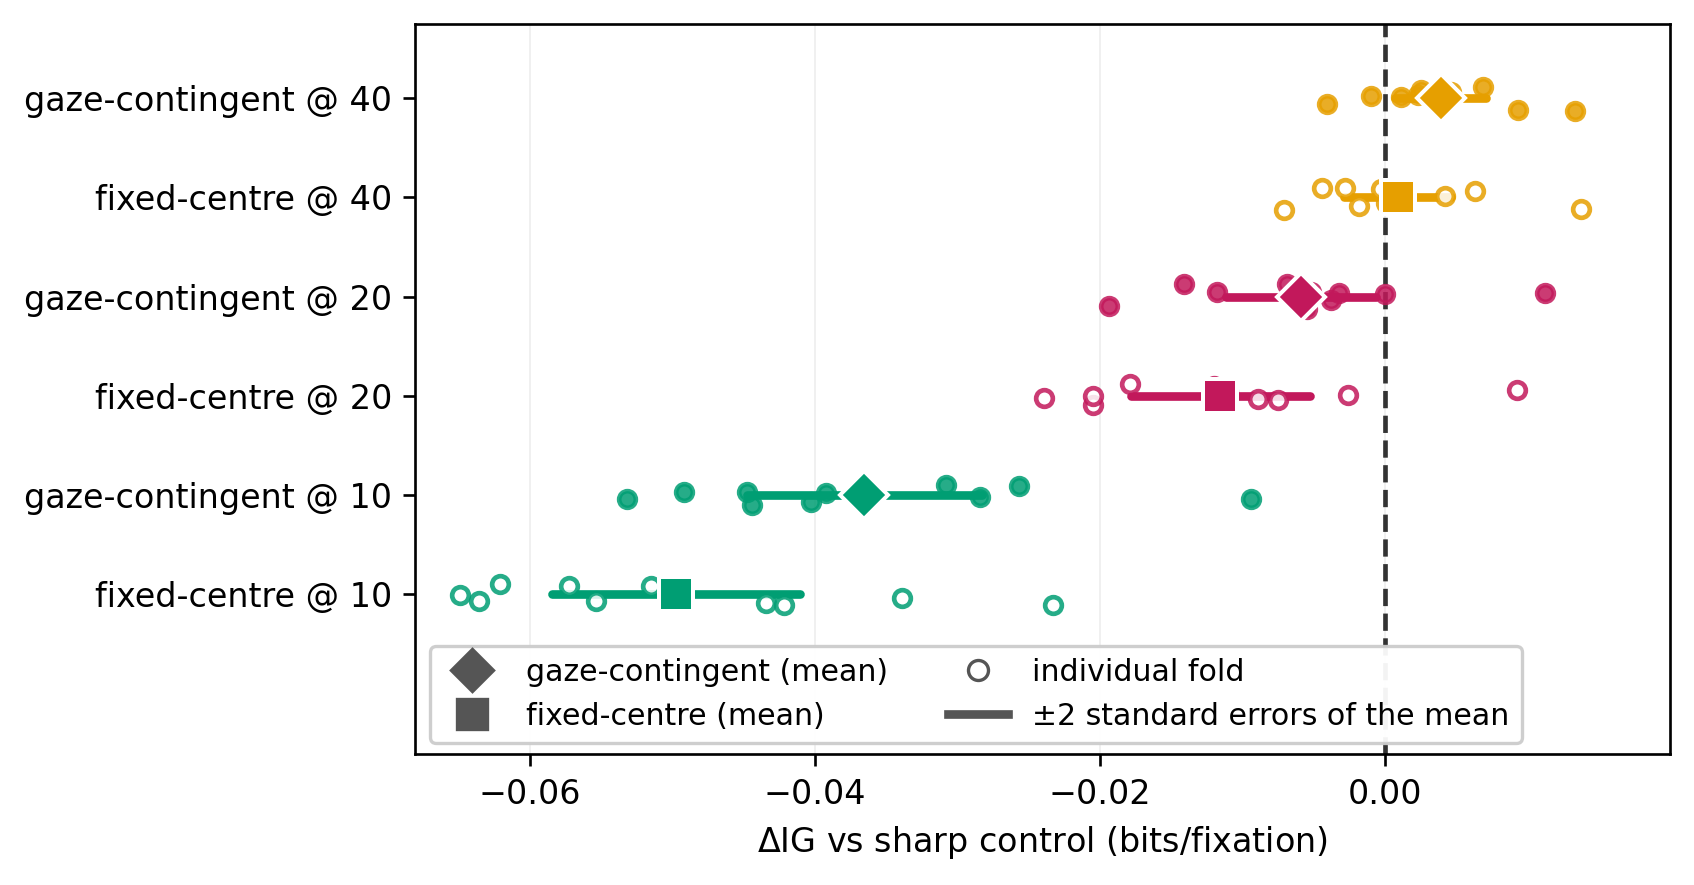
\includegraphics[width=\textwidth]{foveation_mit1003_initial/figs/fold_paired.png}
  \caption[The six arm-versus-control differences by fold]{The six differences of \tabref{phase17-arms} at fold level. Each circle is one fold, that fold's
    foveated read-out minus the control's over the images held out from both; the marker is the mean
    of the ten.}
  \label{fig:fold-paired}
\end{figure}

\subsection{The gaze-contingency contrast}
\label{subsec:results-gaze-contingency}

The gaze-contingent and the fixed-centre arm at each cutoff apply the identical blur profile, so the
difference between them is what following the gaze contributes with the amount of blur held constant
(\subsecref{arms}). That difference, the
gaze-contingent arm's $\Delta \IG$ minus the fixed-centre arm's at the same cutoff, is the
\emph{gaze-contingency term}.
It grows as the periphery degrades, from $+0.0030 \pm 0.0027$~bits at $f_{c0} = 40$ to
$+0.0057 \pm 0.0023$ at $20$ and $+0.0132 \pm 0.0040$ at $10$.

All three differences at a cutoff are taken against the same control on the same fixations, so they add,
the gaze-contingent arm's difference from the control being the fixed-centre arm's difference
plus the gaze-contingency term. Read that way, at $f_{c0} = 10$ the blur costs $0.0497$~bits and
following the gaze returns $0.0132$ of it, and at $20$ it costs $0.0115$ and returns $0.0057$.
Degrading the periphery costs the model, and putting the sharp region where the eye is gives part of
that cost back.

The gaze-contingent arm sometimes delivers the saccade target inside its sharp disc, which would explain
the term. That disc shrinks from $103.5$~px to nothing across the three cutoffs, and the
gaze-contingency term is largest at $f_{c0} = 10$, where the disc has closed.
Whatever produces the term requires the degradation to follow the gaze, and grows as the periphery is
degraded further.

\subsection{Where the cost falls}
\label{subsec:results-diagnostics}

The diagnostics of \subsecref{stats-plan} are computed on the validation split at the same reporting
epoch, pairing the two arms of each contrast on identical fixations.
The map-level diagnostics assign the strong-cutoff loss to spreading rather than to mislocation, the two
arms' AUC at $f_{c0} = 10$ differing by $0.0017$.
At $f_{c0} = 10$ the foveated arm's probability maps carry $0.043 \pm 0.012$~bits more entropy than the
control's, while its predicted mode does not move measurably, against a mode-to-fixation distance of
$191$~px in both arms.
At $f_{c0} = 20$ the same pattern is a quarter the size ($+0.011$~bits), and at $f_{c0} = 40$ the
difference is $-0.003$~bits.
A map spread evenly over the pixels of an MIT1003 stimulus would carry about $19.5$~bits and the
control's carry $17.0$, so $2.5$~bits is what concentrating the density achieves. Against that, none of these
differences reaches $2\%$.

The paired difference, which is a difference in log-likelihood as well
(\subsecref{metrics}), is binned by saccade amplitude with the bin edges at the sharp radii of
\eqnref{sharp-radius}, so every bin lies wholly inside or wholly outside an arm's sharp disc
(\subsecref{sharp-radius}; \figref{stratified-amplitude}).
At $f_{c0} = 40$ the profile shows no step at the $103.5$~px radius; pooling each fold's bins into the two
regions gives $+0.002 \pm 0.007$~bits inside the disc and $+0.005 \pm 0.005$ outside, a difference of
$+0.003 \pm 0.010$.
At $f_{c0} = 10$, where no disc exists, the cost deepens with amplitude and reaches
$-0.149 \pm 0.051$~bits beyond $500$~px.

Stratifying by fixation index tests the expectation that a gaze-contingent cost should build along the
scanpath (\figref{stratified-fixation-index}).
At $f_{c0} = 10$ it does the opposite, with the cost deepest over the first two scored fixations and
down to a fifth of that by the tail, while the two milder cutoffs show no comparable trend.
Neither the saccade amplitude nor the control's own level accounts for it. Mean saccade amplitude
\emph{rises} along the scanpath, from $149$ to $208$~px, and the cost at this cutoff deepens with
amplitude, so amplitude on its own would predict a cost that grows where the measured one shrinks. The
control's information gain falls from $1.80$ to about $1.45$~bits, so there is less to lose late in a
scanpath than early, and the cost shrinks faster than that. Taken as a share of the control's level it
runs from $2.9\%$ over the first scored fixation to $0.8\%$ over the ninth and later.
The rest is consistent with the earliest predictions having the
least history to condition on, so the image carries most of the prediction there, while later
predictions draw on a longer history, which the foveation leaves untouched.

\begin{figure}[tbp]
  \centering
  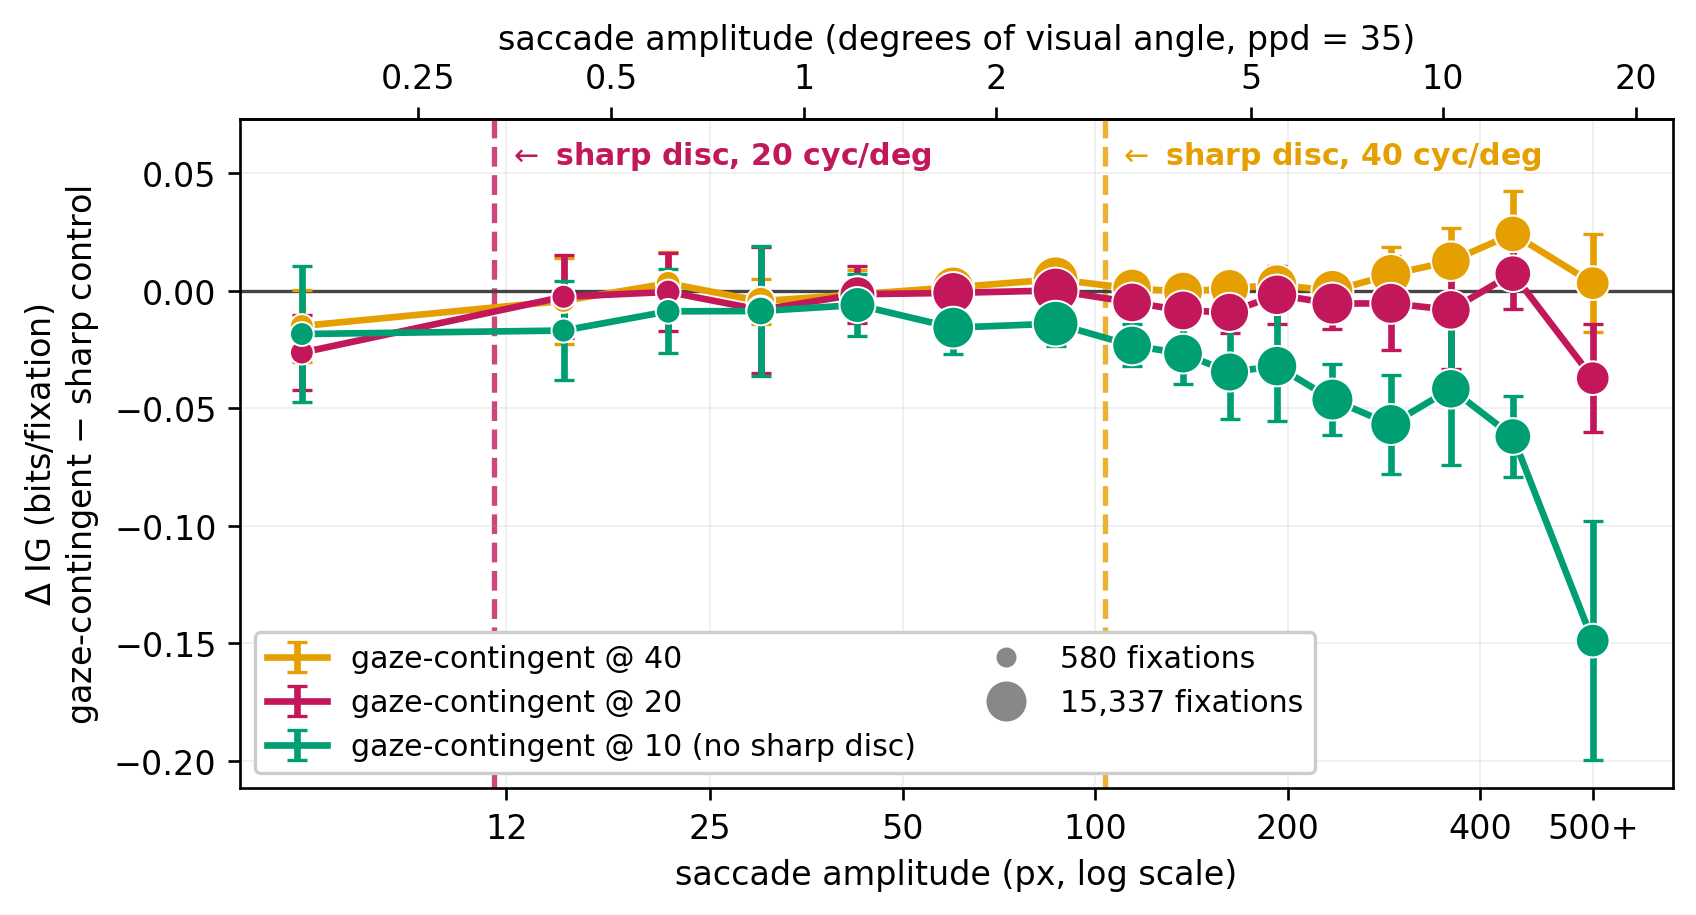
\includegraphics[width=\textwidth]{foveation_mit1003_initial/figs/stratified_amplitude.png}
  \caption[Information-gain difference by saccade amplitude]{The information-gain difference by
    saccade amplitude on the validation split, with each point and bar taken across the ten folds. The
    dashed lines are the sharp radii of \eqnref{sharp-radius}. The last bin is open-ended and holds
    every saccade beyond $500$~px.}
  \label{fig:stratified-amplitude}
\end{figure}

\begin{figure}[tbp]
  \centering
  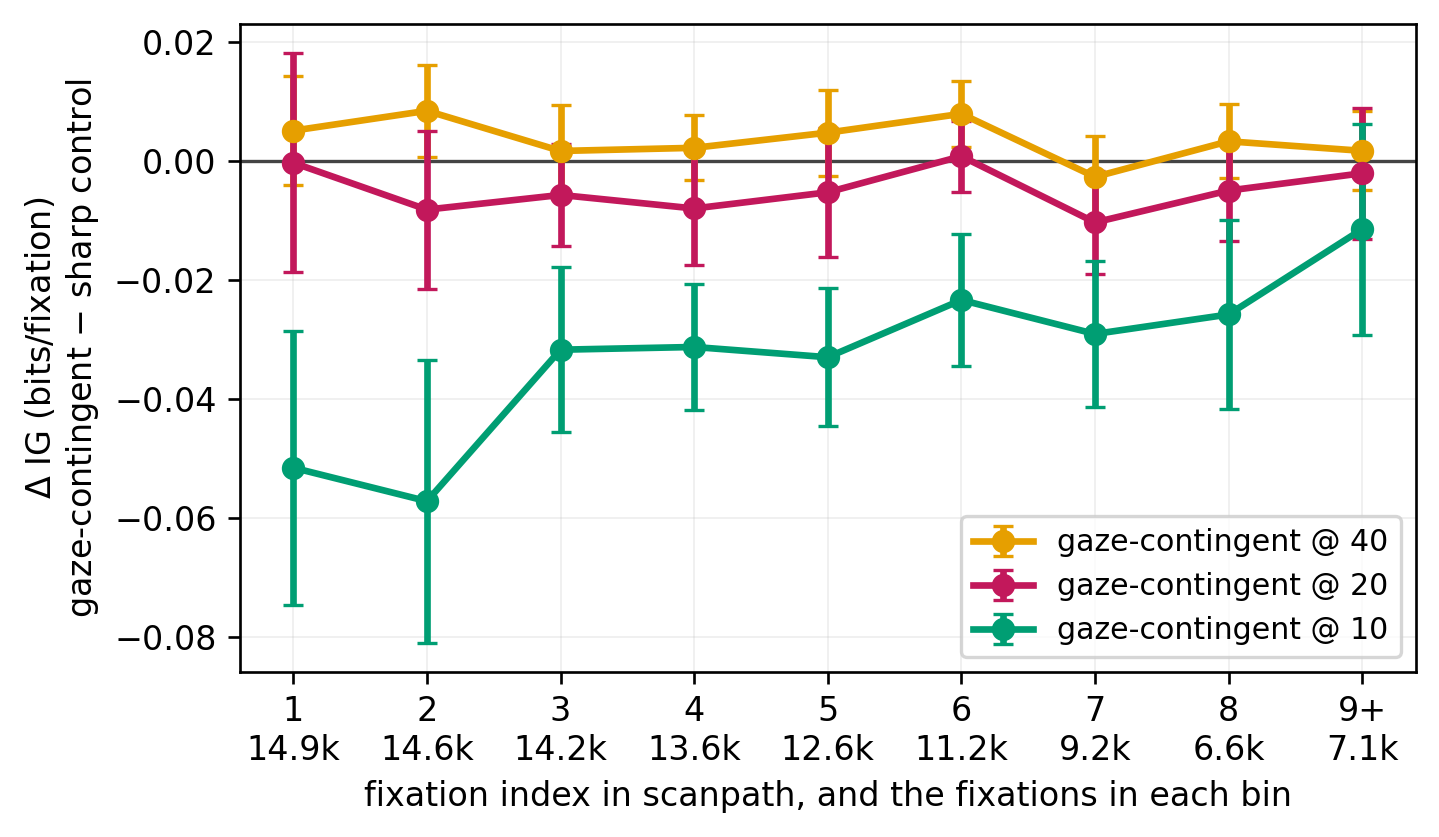
\includegraphics[width=0.85\textwidth]{foveation_mit1003_initial/figs/stratified_fixation_index.png}
  \caption[Information-gain difference by fixation index]{The information-gain difference by fixation index on the validation split, counting from the
    first free fixation onwards (\subsecref{mit1003}); fixations nine and later are pooled.}
  \label{fig:stratified-fixation-index}
\end{figure}

\section{Per-image variation in model fit}
\label{sec:results-per-image}

This section reports how \dg{}'s per-image performance varies with the fixation entropy of
\subsecref{difficulty-proxies}.
The model is the pretrained \dg{}, and the sample is every MIT1003 stimulus under the protocol of
\subsecref{mit1003}.
\figref{per-image-scatter} plots the entropy against each of the four metrics, with Pearson's
product-moment $r$ and Spearman's rank $\rho$ over each panel.

\begin{figure}[tbp]
  \centering
  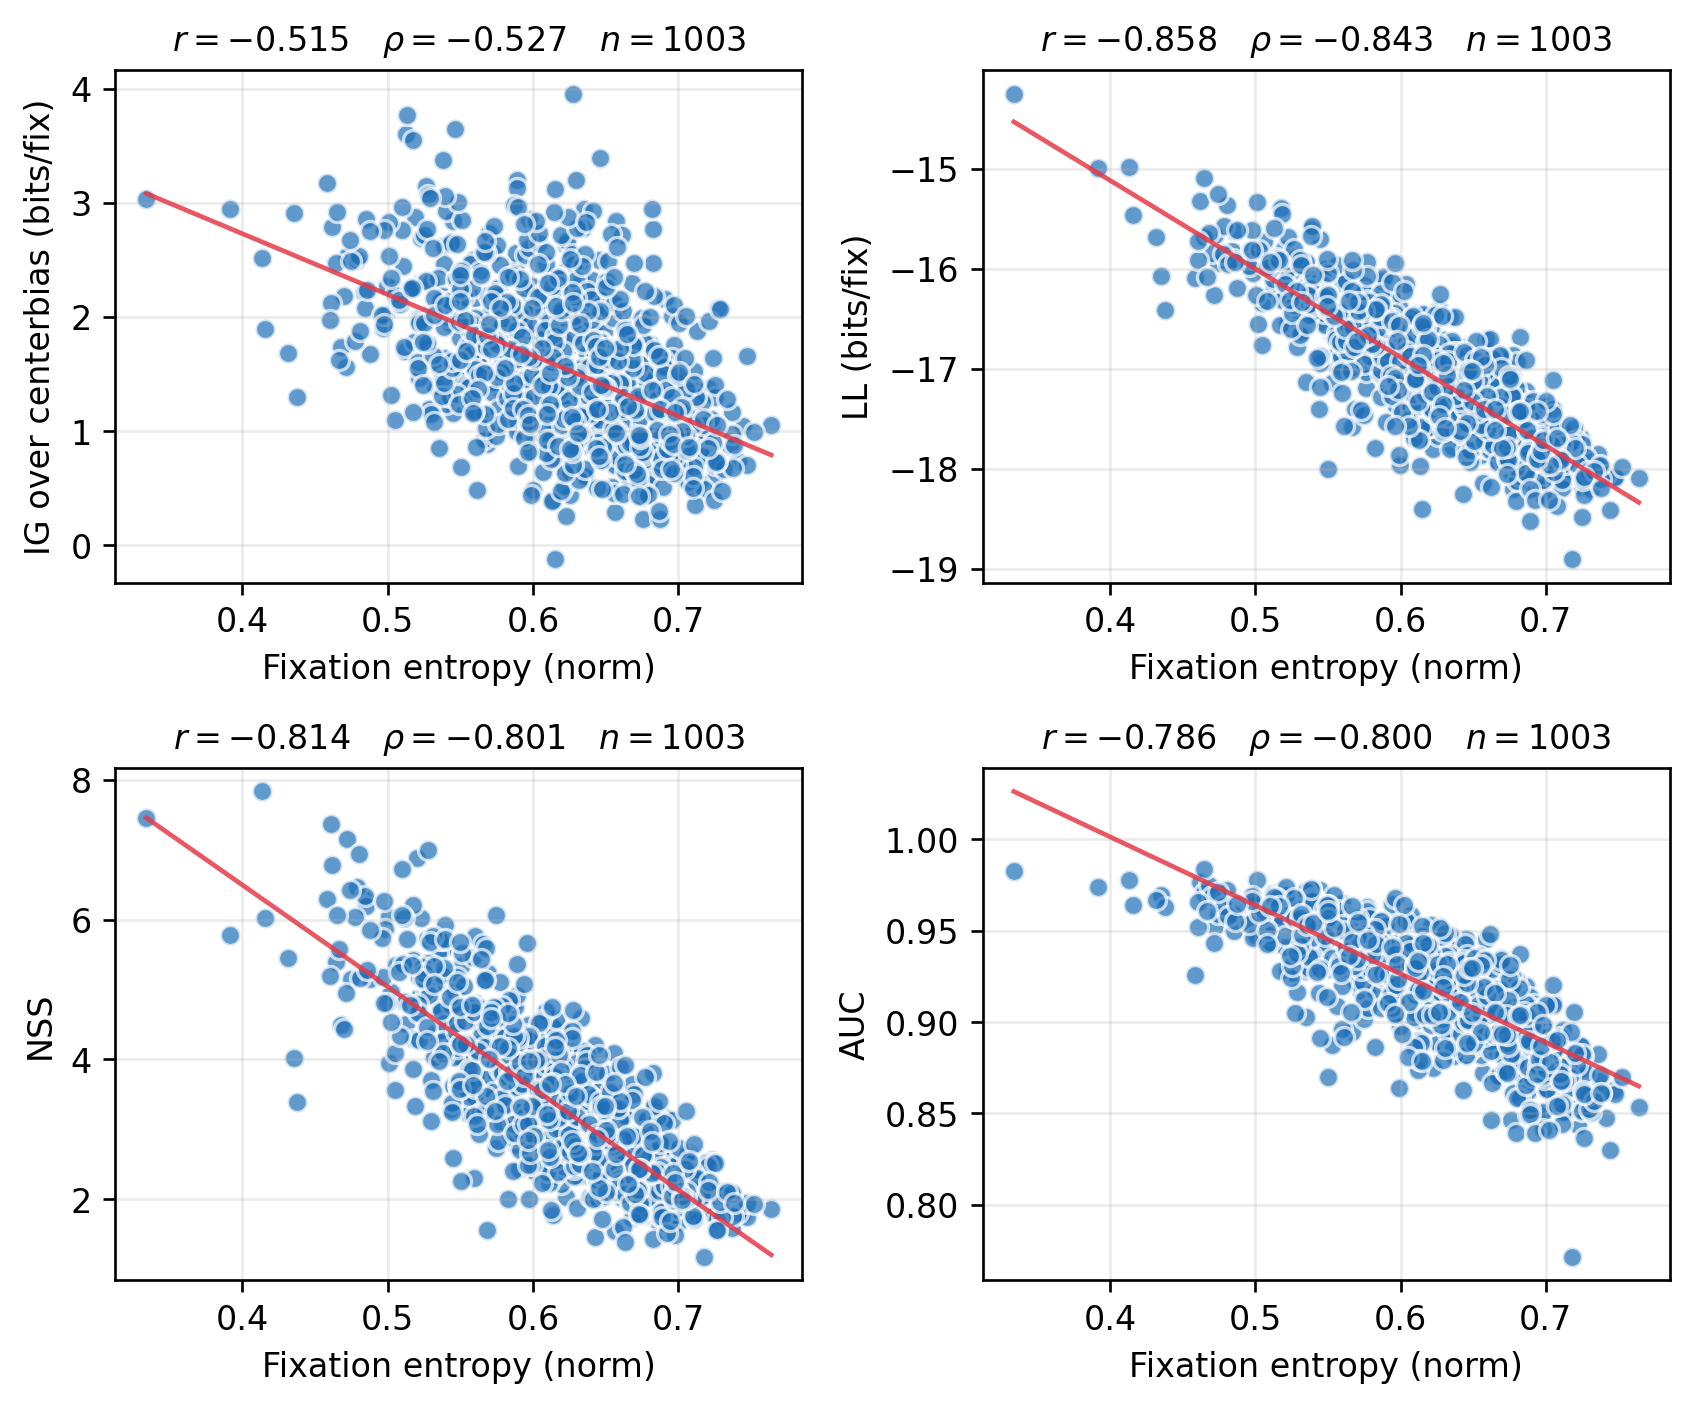
\includegraphics[width=0.88\textwidth]{per_image_diagnostic_initial_1003/scatter.png}
  \caption[Fixation entropy against model fit]{The fixation entropy of \eqnref{fix-entropy} against each of the four per-image metrics, one
    point per stimulus with a least-squares line, for the pretrained \dg{}; $r$ is Pearson's and
    $\rho$ Spearman's.}
  \label{fig:per-image-scatter}
\end{figure}

Fixation entropy runs against every metric, the direction \subsecref{difficulty-proxies} anticipates,
and most strongly against the log-likelihood.
Part of this is a property of the metric rather than of the model.
A likelihood rewards a concentrated density, so when the fifteen subjects looked at the same few places
any model that puts its mass there scores well, and when they looked everywhere none can.
The correlation therefore tracks how hard an image is to score on as much as how well \dg{} does on it.

Per-fixation information gain over the 1003 stimuli ranges from $-0.13$ to $3.96$~bits and AUC from $0.77$ to $0.98$.
\figref{extremes-high} shows the three highest stimuli by information gain and \figref{extremes-low}
the three lowest, with each stimulus's IG, NSS and AUC in the caption.
At the high end a region away from the image centre holds three-quarters of the subjects.
Stimulus $750$ is the one image where \dg{} scores below the centerbias.
The flower the subjects fixated sits at the image centre, where the centerbias already puts its mass,
so the prior that \dg{} is measured against is at its strongest there.

\begin{figure}[tbp]
  \centering
  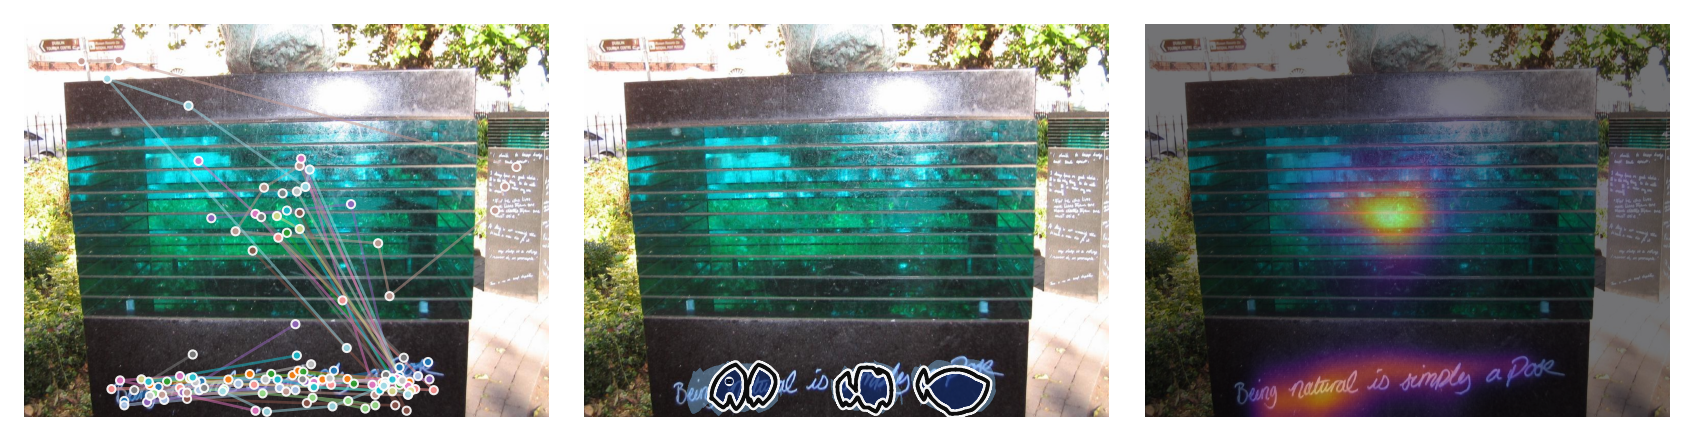
\includegraphics[width=\linewidth]{consensus_panels/consensus_stim0128.png}\\[3pt]
  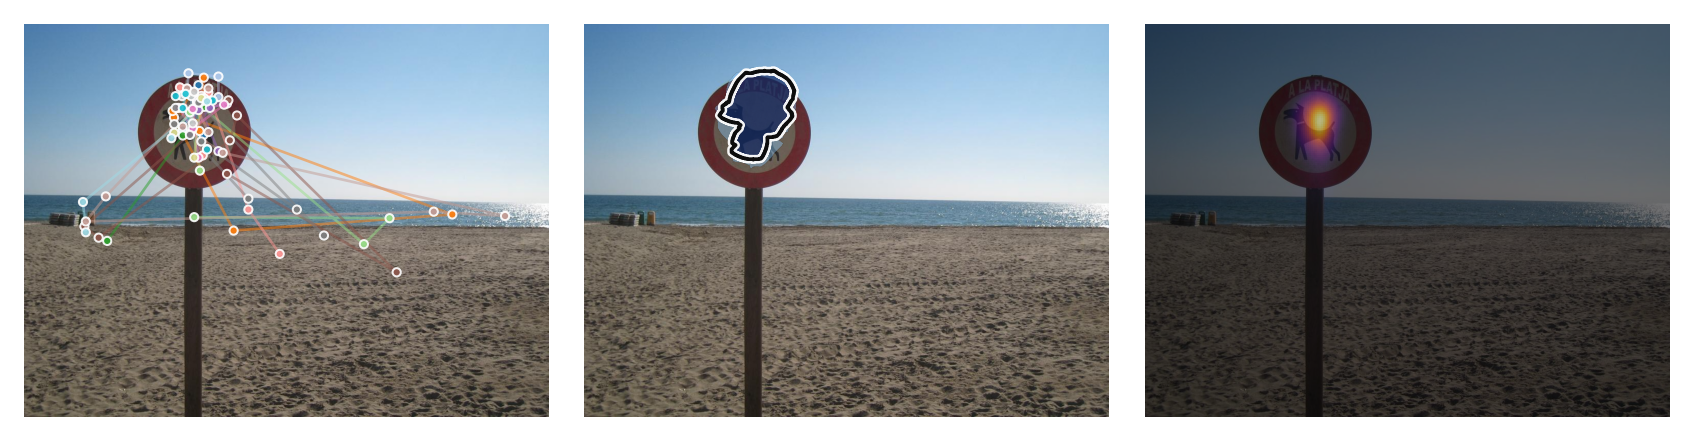
\includegraphics[width=\linewidth]{consensus_panels/consensus_stim0704.png}\\[3pt]
  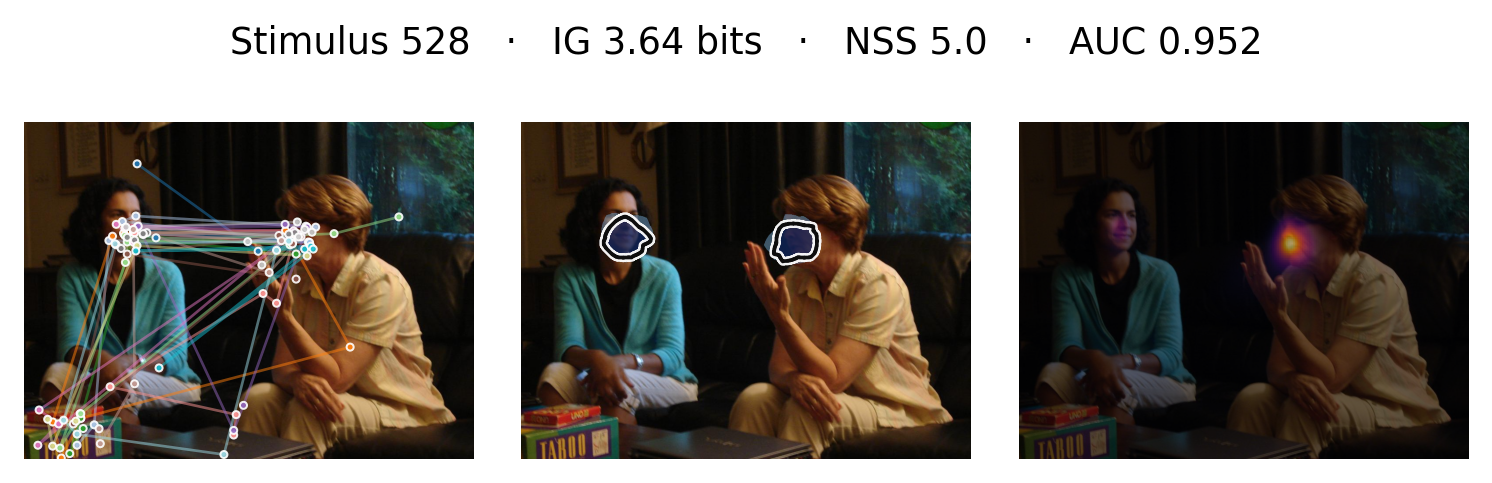
\includegraphics[width=\linewidth]{consensus_panels/consensus_stim0528.png}
  \caption[The three highest stimuli by information gain]{The three stimuli with the highest per-fixation
    information gain, top to bottom: $128$ ($3.96$~bits, NSS $3.4$, AUC $0.931$), $704$ ($3.77$~bits,
    $5.7$, $0.968$) and $528$ ($3.64$~bits, $5.0$, $0.952$). In each row, left to right: every subject's
    scanpath on that stimulus; the consensus regions (Appendix~\ref{app:consensus}); \dg{}'s
    probability map given a single fixation at the image centre.}
  \label{fig:extremes-high}
\end{figure}

\begin{figure}[tbp]
  \centering
  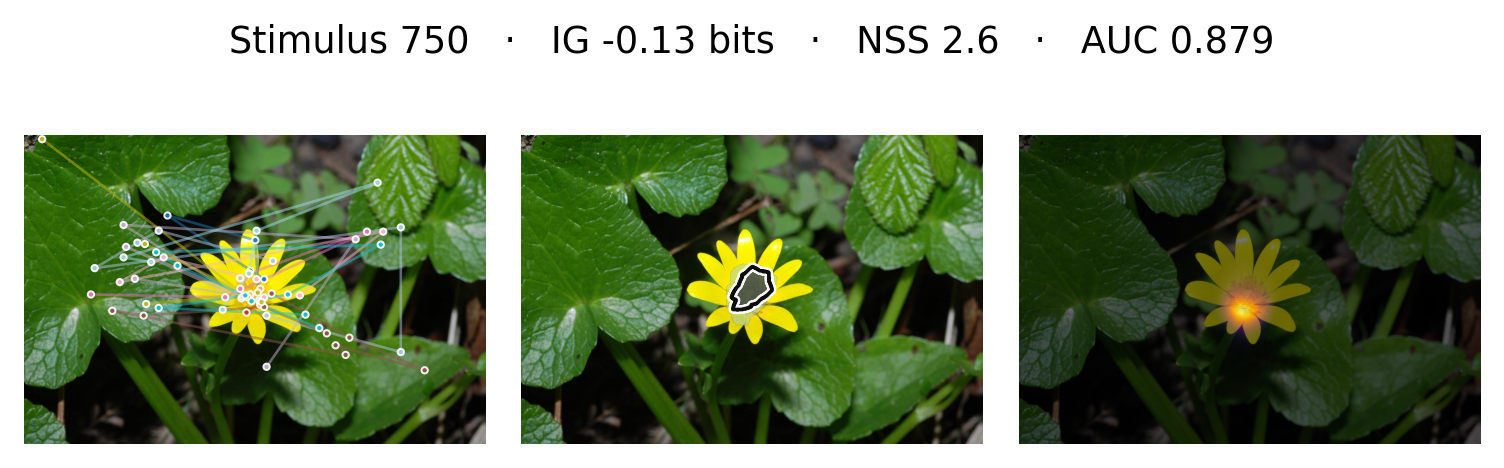
\includegraphics[width=\linewidth]{consensus_panels/consensus_stim0750.png}\\[3pt]
  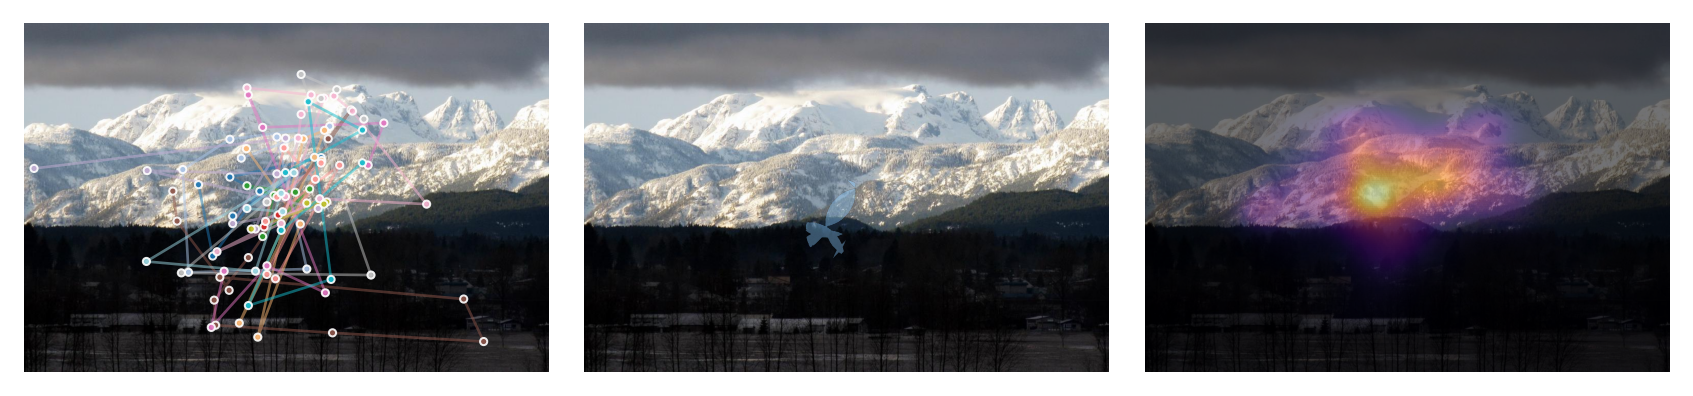
\includegraphics[width=\linewidth]{consensus_panels/consensus_stim0639.png}\\[3pt]
  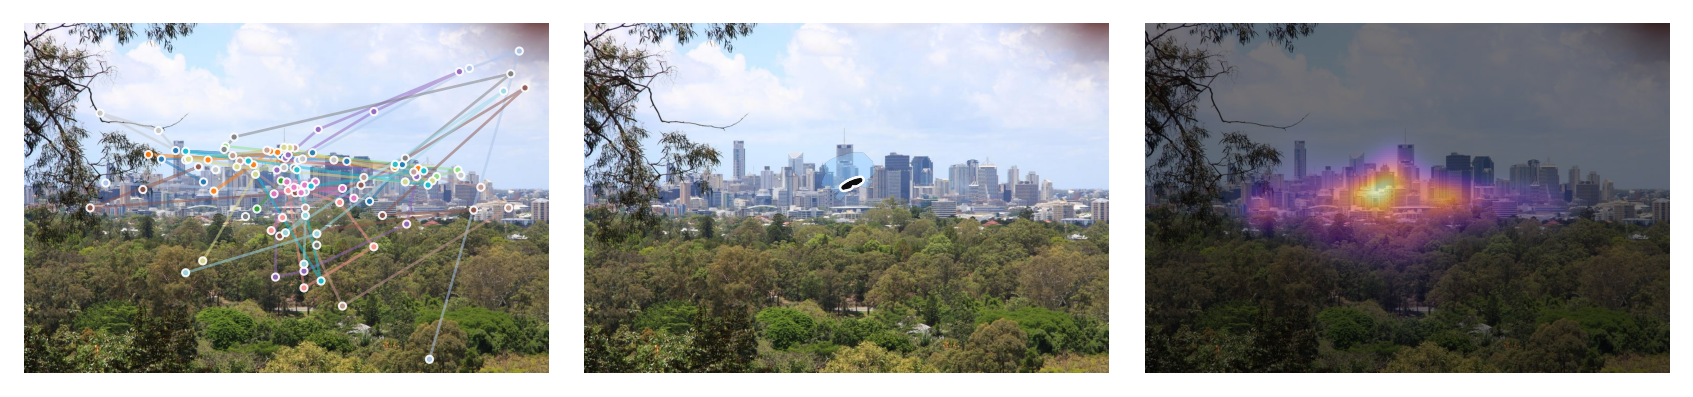
\includegraphics[width=\linewidth]{consensus_panels/consensus_stim0489.png}
  \caption[The three lowest stimuli by information gain]{The three stimuli with the lowest per-fixation
    information gain, top to bottom: $750$ ($-0.13$~bits, NSS $2.6$, AUC $0.879$), $639$ ($0.23$~bits,
    $1.7$, $0.849$) and $489$ ($0.23$~bits, $1.8$, $0.846$). Panels as in \figref{extremes-high}.}
  \label{fig:extremes-low}
\end{figure}

\chapter{Discussion}
\label{ch:discussion}

\section{The foveation result}
\label{sec:disc-finding}

Gaze-contingent input foveation at human acuity costs nothing measurable. The difference at
$f_{c0} = 40$ is at most $0.0071$~bits per fixation, under $1\%$ of what the sharp control gains over the
centerbias, and a loss appears once the blur is pushed past human acuity (\subsecref{results-arms}). At
the coarse cutoffs the map-level diagnostics assign the loss to spreading rather than to mislocation, the
maps carrying more entropy at $f_{c0} = 20$ and $10$ while AUC moves by at most $0.002$
(\subsecref{results-diagnostics}).

At human acuity the foveation removed nothing the fit depended on measurably. At the coarser cutoffs it
did. The model draws on detail the coarser blur removes, by about $2\%$ of its gain over the centerbias at
$f_{c0} = 10$, and the per-fixation cost deepens with saccade amplitude (\figref{stratified-amplitude}); the measured cost is an
upper bound on what the discarded detail was worth, provided the frozen backbone --- fitted to sharp
photographs --- is no better on foveated input than on sharp. Nothing here tests that; unfreezing the
backbone would (\secref{disc-limits}).

The fixed-centre arms separate degrading the periphery from letting the sharp region follow the gaze.
With the same blur held at the image centre, the arm sits below the gaze-contingent one at every cutoff,
and the difference between the two, the gaze-contingency term, grows from $0.003 \pm 0.003$~bits at
$f_{c0} = 40$ to $0.013 \pm 0.004$ at $10$ (\subsecref{results-gaze-contingency}). Degrading the periphery is what costs, and letting the sharp
region follow the gaze gives part of that cost back. What produces that return is not established.

\dg{}'s authors put a related question to the read-out (\secref{position}) and found that \enquote{the
distance to the fovea plays only a minor role for guiding free-viewing gaze on average}
\citep{kummerer2022deepgaze3}. Those variants were fed the same
sharp image, so the test held the available information fixed. The result here is the input-level
counterpart. At human acuity, changing the information itself leaves performance where it was, within
what this design can measure.

\section{The per-image diagnostic}
\label{sec:disc-per-image}

\dg{}'s fit varies more from image to image than any arm differs from another, and that variation
follows how far the fifteen subjects spread (\secref{results-per-image}). \subsecref{stats-plan} takes every difference inside an image for that
reason, and the diagnostic characterises what the pairing removes. Part of that spread belongs to the
metric (\secref{results-per-image}), so a low per-image score is not on its own evidence that the model
failed there.

\section{Limitations}
\label{sec:disc-limits}

Several limitations bound what the comparison resolves and how far the result reaches.

\begin{itemize}
  \item \emph{The backbone is frozen.} The features every arm reads were learned on sharp photographs,
    and only the read-out adapts to the foveated input. Unfreezing part of the backbone, or training it
    on foveated input from the start, is untested (\secref{disc-future}).
  \item \emph{The evaluation is scored on human scanpaths.} Every history the model conditions on is a
    human scanpath and every scored location is a human fixation (\subsecref{metrics}), so the foveated
    model's sharp region always sits where a subject was looking, and the model never has to find a target
    with its own degraded periphery. What the comparison measures is the value of peripheral detail for
    predicting the next human fixation from a human history. Whether a foveated model would produce
    human-like scanpaths on its own is a separate question this design does not ask.
  \item \emph{Native resolution is a shift for the backbone.} \dg{} was released fitted on resized
    stimuli, and the arms here read each stimulus at its own size so that the sharp region stays a disc
    (\subsecref{gp-model}). Every arm carries that shift equally, so it is not a difference between
    them, and nothing here tests whether it interacts with the foveation.
  \item \emph{Faithful foveation is mild on lab-sized images.}
    Because acuity falloff is set in degrees and an MIT1003 stimulus spans $29^\circ$ along its long
    side, the foveation at the human setting leaves a third of all saccade targets untouched.
    Differences large enough to read off without ten-fold pairing appear only at coarser-than-human
    strengths, so the argument rests on the shape of the dose--response and on the fixed-centre contrast
    rather than on the size of any single point.
  \item \emph{A single dataset.} All results are on MIT1003 free-viewing by adults; other datasets and
    tasks (visual search, other populations) may behave differently.
  \item \emph{Fifteen subjects, thinly described.} MIT1003 provides fifteen subjects for every
    image, described in a single sentence as males and females aged between 18 and 35
    \citep{judd2009mit1003}. Each likelihood in \chref{results} is therefore measured against those
    fifteen people rather than against the expected value more subjects would estimate, and age is
    given only as that range, while first language and script direction are not recorded at all, so
    none of them can be controlled for.
  \item \emph{The falloff shape is fixed.} Every foveated arm inherits the same half-acuity eccentricity
    $e_2 = 2.3^\circ$ (\subsecref{gp-model}). Human-strength here means human-strength for
    one acuity profile, and the thesis does not test others.
  \item \emph{The mechanism models acuity falloff only.} Resolution is not the only peripheral limit. An
    object resolvable in isolation becomes hard to identify when others lie near it, \emph{crowding}
    \citep{strasburger2011peripheral}, so degrading peripheral resolution reproduces part of peripheral
    vision and not all of it.
  \item \emph{Fixation duration is not represented.} \dg{} takes fixation coordinates only
    \citep{kummerer2022deepgaze3}, so if foveating the input changed how long subjects dwelled at each
    location without changing which locations they chose, this evaluation would not register it.
\end{itemize}

\section{Future work}
\label{sec:disc-future}

The most direct extension is replication. Every number reported here comes from one dataset, so the
dose--response of \secref{results-foveation} may be a property of the mechanism or a property of MIT1003.
Running the same arms and the same $f_{c0}$ sweep on a second dataset of adult free-viewing gaze would
separate the two. The evaluator already accepts any model matching the \dg{} forward signature
(Appendix~\ref{app:eval}), so the work is a loader and a centerbias fitted to the new stimuli
(\subsecref{metrics}). The dataset must record its viewing geometry, because without pixels-per-degree
the two cannot be foveated at a matched strength in degrees (\subsecref{gp-model}), leaving display
scale confounded with foveation.

Unfreezing part of the backbone would separate the detail the foveation discards from the DenseNet's
unfamiliarity with blurred input, which the cost at the coarse cutoffs mixes (\secref{disc-limits}).
Compute kept it out of scope, and it would change what the comparison measures, since a difference
between arms would then include what each backbone learned from its own input.

The longer-range question is developmental, whether a model's \emph{learning trajectory} recapitulates
the development of human gaze, which changes measurably with age
\citep{helo2014maturation, acik2010developmental}. This thesis makes no claim that a read-out's training
trajectory resembles that development; the front-end makes the comparison possible, and testing it needs
a developmental eye-tracking dataset that records its viewing geometry, which the replication above also
requires.

Smaller extensions follow from constraints already stated. A transformer host would test whether the dose--response
survives a change of generator (\secref{position}). A duration channel would let the evaluation register
a change in dwell time (\secref{disc-limits}).

\chapter{Conclusion}
\label{ch:conclusion}

This thesis added a biological constraint that \dg{} lacked, the foveated eye, and measured
its effect.
The arms were trained on MIT1003 against an otherwise-identical sharp-input control. At human acuity
the foveated input differs from sharp by at most $0.0071$~bits per fixation, under $1\%$ of what the
sharp control gains over the centerbias. A third set of arms, holding the
same blur fixed at the image centre, isolates gaze-contingency. The fixed-centre arms sit below the
gaze-contingent ones at every cutoff, by $0.003 \pm 0.003$~bits at human acuity and $0.013 \pm 0.004$ at
the coarsest, so the gap widens as the periphery is degraded further.

At human acuity the foveation removed nothing the fit depended on measurably. Past it, at the cutoffs
where the blur is stronger than a human eye applies, it did, within what a frozen backbone lets the
comparison attribute to the input (\secref{disc-limits}), and the cost appears as a loss of concentration
rather than of ranking.

Across images, \dg{}'s fit varies more than any arm differs from another, and that variation follows how
far the fifteen subjects spread; the arm comparison is small against it and is read within images for that
reason. The result rests on one dataset, one acuity profile and a backbone fitted to sharp photographs.

The foveation experiment leaves a working front-end.
The immediate open direction is replication, running the same comparison on a second adult dataset to
show whether the dose--response reported here is a property of the mechanism or of MIT1003. Beyond it
lies the developmental question, whether training a foveated model recapitulates, along its learning
trajectory, the child-to-adult changes in human gaze. This front-end was built to make that question
answerable.


% ----- Appendices -------------------------------------------------------
\appendix
\chapter{Implementation and reproducibility}
\label{app:impl}

This appendix collects the implementation and reproducibility detail referred to from \chref{methods}.
Code and result artefacts are at \url{https://github.com/W00DSRULES/bio-inspired-foveation-in-dg3}.
Modules named below belong to the \texttt{tez\_deepgaze} package; scripts are named by file.

\section{Dataset access and cross-validation}
\label{app:data}

The dataset is the \pth{MIT1003_initial_fix_consistent} variant of MIT1003, built once by
\texttt{fetch\_mit1003.py --with-initial} and read through \texttt{pysaliency}'s
\pth{get_mit1003_with_initial_fixation}. It returns each scanpath as a variable-length sequence with the
forced central fixation at index~$0$. With \texttt{start\_fixation = 1} that fixation is history only
and every free fixation is scored, the protocol of \citet{kummerer2022deepgaze3} and of \subsecref{mit1003}.
Training and evaluation both select the variant with \texttt{--dataset-variant initial}. The plain
\texttt{get\_mit1003} loader drops the central fixation on load, so the same \texttt{start\_fixation}
then skips the first free fixation as well; it is not used for any number reported here.

Folds are built via \texttt{pysaliency}'s \pth{filter_datasets} module with
\pth{crossval_folds=10}, \pth{val_folds=1} and \pth{test_folds=1}.
The splitter hardcodes \texttt{RandomState(42)} internally, so the shuffle is fixed whatever seed a
caller passes (the \dg{} training notebook passes none), which is why the two
partitions coincide (\subsecref{cv-split}). For each fold $k \in \{0, \ldots, 9\}$ the split has eight
training, one validation, and one test fold.

\section{Evaluator and metrics}
\label{app:eval}

\texttt{evaluate.py:run} accepts any module matching the \dg{} forward signature and never inspects its
class, so one code path produces the pretrained baseline, the sweep tables and the stratified analysis
alike. The per-epoch validation inside the training loop is a separate, lighter loop, pooled per fixation
where the evaluator averages per image; it supplies only the curves of \figref{training-curves}.

NSS is not taken from the \texttt{deepgaze\_pytorch} library. Its released implementation
unpacks \texttt{torch.std\_mean} in the wrong order, so it divides the centred density by the mean where
\eqnref{nss} divides by the standard deviation. \texttt{evaluate.py} therefore carries a local copy with
that line corrected, and every NSS in this thesis comes from it. The pinned dependency set records the
library version but not this substitution, so it is stated here.

The centerbias is the precomputed \texttt{centerbias\_mit1003.npy} from the \dg{} release. At evaluation
time \texttt{centerbias.py} resizes it to each stimulus by nearest-neighbour zoom and renormalises in
log-space via \texttt{logsumexp}, so the result is a proper log-probability density summing to one over
image pixels.

\section{Consensus regions}
\label{app:consensus}

The figures of \chref{results} draw inter-subject agreement as a \emph{consensus region}: the part of
the image that at least three-quarters of the subjects fixated within $2^\circ$ of, enclosed by a
contour, with a second contour for the $90\%$ core. Two degrees is the foveal radius of
\secref{foveated-vision}, so a pixel inside the region is one those subjects saw foveally. The region is
a way of drawing agreement rather than a measure of it; the scalar the correlations of \chref{results}
read is the entropy of \eqnref{fix-entropy}.

Agreement is summarised by the \emph{consensus count map}, an array
the shape of the image whose value at each pixel is the number of distinct subjects who fixated within
a radius $R$ of it. For a stimulus of shape $(H, W)$, $N$ subjects, and radius $R$,

\begin{equation}
  C(y, x) \;=\; \sum_{s=1}^{N} \mathbf{1}\!\left[
    \exists\, (x_i, y_i) \in \mathcal{F}_s \;:\; \norm{(y, x) - (y_i, x_i)} \leq R
  \right],
  \label{eq:consensus-count}
\end{equation}

where $\mathcal{F}_s$ is subject $s$'s fixation set and $\mathbf{1}[\cdot]$ the indicator function.
Thresholding at fixed fractions of the subject count gives the two contours the figures draw:

\begin{equation}
  M_{0.75}(y, x) = \mathbf{1}[C(y, x) \geq \lceil 0.75 N \rceil],
  \qquad
  M_{0.90}(y, x) = \mathbf{1}[C(y, x) \geq \lceil 0.90 N \rceil].
  \label{eq:consensus-masks}
\end{equation}

$N$ counts the subjects who fixated the image, so with fifteen subjects the two thresholds resolve to
at least twelve and at least fourteen of them. The radius is $R = 70$~pixels throughout, which is
$2^\circ$ at the MIT1003 viewing geometry.

\section{Input-foveation implementation}
\label{app:foveation}

\subsection*{Where the human cutoff \texorpdfstring{$f_{c0} = 40$}{fc0 = 40} comes from}

\subsecref{gp-model} takes $f_{c0} = 40$~cyc/deg as human acuity rather than the ${\sim}50$~cyc/deg
\citet{geislerperry1998} quote in their introduction. The two figures come from different places in the
same paper: the $50$ is a general statement of human resolution, paired with a half-acuity eccentricity of
$2.5^\circ$, whereas the model they fitted is a contrast-threshold law,

\begin{equation}
  CT(f, e) \;=\; CT_0 \exp\!\left(\alpha f \, \frac{e + e_2}{e_2}\right).
  \label{eq:gp-contrast}
\end{equation}

$CT$ is the faintest contrast at which a grating of spatial frequency $f$ is still visible at
eccentricity $e$. Of its three fitted constants, $CT_0$ is that threshold at the fovea for a coarse
grating, $\alpha$ sets how fast the threshold rises as the grating gets finer, and $e_2$ how fast it
rises away from the fovea.

The bracket $(e + e_2)/e_2$ is the eccentricity penalty, equal to one at the fovea and doubling at
$e = e_2$. At the fovea it drops out, leaving $CT(f, 0) = CT_0 \exp(\alpha f)$.

A cutoff is a frequency above which nothing is visible however the image is drawn, which is where the
threshold reaches $CT = 1$, the maximum contrast. Setting $CT = 1$ in the foveal case and solving for
$f$ leaves the foveal cutoff fixed by two fitted constants alone:

\begin{equation}
  f_{c0} \;=\; \frac{\ln(1/CT_0)}{\alpha}.
  \label{eq:fc0-derivation}
\end{equation}

Solving the same way at general $e$, keeping the bracket, returns \eqnref{gp-acuity}, so the acuity law
\secref{foveation} is built on is this fitted law rearranged rather than a second assumption.

\citet{geislerperry1998} fit \eqnref{gp-contrast} to the contrast-sensitivity measurements of
\citet{robson1981}, obtaining $\alpha = 0.106$, $e_2 = 2.3^\circ$ and $CT_0 = 1/64$, and report that the
same $\alpha$ and $e_2$ also fit two further published contrast-sensitivity studies with a different
minimum contrast threshold each: $CT_0 = 1/75$ for \citet{arnow1996} and $1/76$ for \citet{banks1991}.
\eqnref{fc0-derivation} turns those three thresholds into $39.2$, $40.7$ and $40.9$~cyc/deg
respectively, a mean of $40.3$ with a standard deviation of $0.9$. That spread is a check on how much the foveal cutoff moves when the threshold is
measured on different subjects, not three independent refits: $\alpha$ and $e_2$ are held fixed across
all three, and only $CT_0$ varies. The $f_{c0} = 40$ used here and the $e_2 = 2.3^\circ$ of
\subsecref{gp-model} therefore come from the same fit.

\subsection*{Viewing geometry and the pixels-per-degree constant}

\subsecref{gp-model} uses $\ppd = 35$ for MIT1003. \citet{judd2009mit1003} report viewing
\enquote{approximately two feet from a 19 inch computer screen of resolution $1280 \times 1024$}, which
works out to $\ppd \approx 36.1$. The \dg{} release states $35$~pixels per degree for the same dataset
\citep{deepgazepytorch}, which is the value used here.
In pixel space $\ppd$ enters the blur only as an additive offset: substituting
$e_{\text{deg}} = e_{\text{px}}/\ppd$ into \eqnref{gp-acuity} and \eqnref{frac-level} gives

\begin{equation}
  L(e_{\text{px}}) \;=\; \log_2 \frac{e_{\text{px}} + e_2\,\ppd}{2 f_{c0} e_2},
  \label{eq:level-pixels}
\end{equation}

so the far field does not depend on $\ppd$ at all. By \eqnref{level-pixels} the difference between $35$
and $36.1$ shifts the blur by at most $3\%$ in $\sigma$, and by nothing inside the sharp disc, where the
clamp holds $L = 0$.

\subsection*{Implementation}

The space-variant foveation of \secref{foveation} is implemented in \texttt{foveate\_input.py}. The
Geisler--Perry cutoff \eqnref{gp-acuity} is evaluated per pixel from the eccentricity to the current
fixation and the pixels-per-degree constant, converted to cycles-per-pixel, and clamped at the display
Nyquist ($0.5$~cyc/px); the fractional pyramid level \eqnref{frac-level} then indexes a Gaussian pyramid
whose two bracketing levels are blended with triangular weights that sum to one. The pyramid is octave
spaced: level $i$ targets a half-amplitude cutoff of $0.5 \cdot 2^{-i}$~cyc/px, which for a Gaussian of
standard deviation $\sigma$ gives $\sigma_i = 0.375 \cdot 2^{i}$~px, and the levels are built with
\texttt{torchvision}'s differentiable \texttt{gaussian\_blur}. The transform is geometry-preserving
(pixels do not move), so the output is never a log-polar warp. In the gaze-contingent arms the image is
foveated around the most recent fixation of the history before each forward pass; the pyramid is built
once per image and reused across the fixations scored on it.

\section{Training internals}
\label{app:training}

Read-out fine-tuning is implemented in \texttt{foveated\_train.py}. \pth{freeze_for_head_training} sets
\texttt{requires\_grad=False} on the DenseNet backbone (\texttt{features}) and the finalizers and places
every submodule in \texttt{.eval()} mode, so BatchNorm running statistics and the finalizer's two learned
parameters, its Gaussian kernel width and its centerbias weight, stay fixed; the saliency, scanpath, and
fixation-selection networks remain trainable.
\texttt{audit\_trainable} asserts that every trainable parameter lies in those three read-out groups and that
the frozen groups contribute none, raising otherwise. The arms differ only in the input handed to the
same training routine: sharp, foveated, or foveated with the centre pinned to the image midpoint for
every fixation.

The optimiser is Adam over the read-out parameters at a base learning rate
of $3 \times 10^{-4}$; \texttt{lr\_for\_epoch} applies the step decay of \subsecref{training-loop},
dividing the base rate by ten at epoch five. Its milestones are absolute, at epochs five, eight and
eleven, so the two later ones fall outside the seven-epoch schedule and never fire.

One image yields about a hundred (history, target) pairs, so the per-image loss is accumulated over
\texttt{micro\_batch} chunks before one optimiser step, and gradients are clipped to unit norm.

Every epoch writes one checkpoint bundle: \texttt{weights.pt}, which holds only the trainable read-out
tensors, since the frozen submodules stay byte-identical to the pretrained weights at every epoch,
\texttt{optimizer.pt} with Adam's moment estimates, and a \texttt{metrics.json} sidecar. The sidecar
records the validation log-likelihood and information gain, the seed, the git commit, and
SHA-256 hashes of \texttt{uv.lock} (which pins every dependency, the \texttt{deepgaze-pytorch} git
revision and the \texttt{pysaliency} release among them), the \texttt{deepgaze3.pth} weights, the
\texttt{centerbias\_mit1003.npy} prior and the cross-validation split file, so a changed input shows as a
hash mismatch.

\section{Cluster execution}
\label{app:cluster}

\texttt{device.py:pick\_device} chooses CUDA, then MPS, then CPU. Every reported run used CUDA on the
NVIDIA \texttt{gpu2} partition of the Goethe-NHR cluster, one Slurm job per arm and fold, from seed $42$.
The driver \pth{foveation_pump.sh} submits the seven-arm matrix of \subsecref{arms}
(sharp, gaze-contingent at $f_{c0} \in \{40, 20, 10\}$ and fixed-centre at the same three
cutoffs, ten folds each, so $70$ jobs). Training was launched as
\begin{center}
\texttt{TEZ\_EPOCHS=7 TEZ\_DATASET\_VARIANT=initial bash} \pth{scripts/slurm/foveation_pump.sh}
\end{center}
and the tables of \chref{results} come from \pth{foveation_sweep_eval.sbatch}, run once per split with
\texttt{TEZ\_EPOCH=5} and \texttt{TEZ\_DATASET\_VARIANT=initial} and scoring the checkpoints with the
evaluator of \secref{eval-framework}; \pth{foveation_sweep_table.py} assembles
\texttt{table.json} and \pth{make_results_figures.py} renders \tabref{phase17-arms} from it. The stratified
diagnostics come from \pth{foveation_stratified.py} at the same epoch on the validation split, and the
per-image diagnostic from \texttt{per\_image\_diagnostic.py --n-stim 1003 --dataset-variant initial}.


% ----- Back matter ------------------------------------------------------
\cleardoublepage
\printbibliography[heading=bibintoc]

\end{document}
